\documentclass[a4paper,10pt]{article}
\usepackage{geometry} %Per impostare i  margini del foglio
 \geometry{
 a4paper,
 total={170mm,257mm},
 left=20mm,
 top=20mm,
 }
%\setcounter{secnumdepth}{1} %per subsection non numerate ma nell'indice
\usepackage[italian]{babel} %Mette in italiano tutte le parole fisse di LaTeX (v. "TITOLO")
\usepackage[utf8]{inputenc} %Gestisce i caratteri accentati
\usepackage{comment} %Per  usare \begin{comment}
\usepackage{amsthm} %per gli ambienti theorem
\usepackage{amsmath} %cose matematiche
\usepackage{amssymb} %cose matematiche
\usepackage{mathrsfs} %per \mathscr
\usepackage{dsfont} %per \mathds{1}
\usepackage{mathtools}
\usepackage{float}
\usepackage{units} %per \nicefrac{}{} 
\usepackage{cancel} %per \cancel{}
\usepackage{caption} %mettere le descrizioni
\usepackage{graphicx} %Importare foto
\usepackage{booktabs}
%\pagestyle{empty} %per togliere il numero della pagina
\usepackage{xcolor} %per \color{} e \textcolor{}{}
\usepackage[dvipsnames]{xcolor}
\usepackage{empheq} 
%\usepackage{enumitem} %Insieme  ai vari \renewcommand per fare elenchi coi numeri belli
\usepackage[shortlabels]{enumitem}
\usepackage{physics} %Per avere \nabla in grassetto
\usepackage[most]{tcolorbox} %Box colorati teoremi
\usepackage{mdframed}
\usepackage{framed}
\usepackage{color,soul} %per evidenziare con il comando highlight \hl
\usepackage{hyperref} %per URL (con \url{}) e hyperlink
\usepackage{tikz} %robe  disegnate
\usepackage{tikz-cd}
\usetikzlibrary{matrix,shapes}
\usepackage{color}
\definecolor{shadecolor}{rgb}{0.902344, 0.902344, 0.902344}
\usepackage{wasysym} %per \lightning
\usepackage{dsfont} %per \mathds{1}



%DA BARABBA%%%%%%%%%%%%%%%%%%%%%%%%%%%%%%%%%%%%%%%%%%%%%%%%%%%%%%%%%%%%%%%%%%%
%\usepackage{tikz}
%\usepackage[unicode=true,pdfusetitle,
% bookmarks=true,bookmarksnumbered=false,bookmarksopen=false,
% breaklinks=false,pdfborder={0 0 1},backref=false,colorlinks=false]
% {hyperref}
\usepackage{changepage}

\usepackage{array}
\usepackage{float}
\usepackage{booktabs}
\usepackage{calc}
\usepackage{units}
\usepackage{mathrsfs}
\usepackage{mathtools}
\usepackage{enumitem}
\usepackage{todonotes}
\usepackage{amsmath}
\usepackage{amsthm}
\usepackage{amssymb}
\usepackage{cancel}
\usepackage{wasysym}
\PassOptionsToPackage{obeyFinal}{todonotes}

\newlist{casenv}{enumerate}{4}
\setlist[casenv]{leftmargin=*,align=left,widest={iiii}}
\setlist[casenv,1]{label={{\itshape\ \casename} \arabic*.},ref=\arabic*}
\setlist[casenv,2]{label={{\itshape\ \casename} \roman*.},ref=\roman*}
\setlist[casenv,3]{label={{\itshape\ \casename\ \alph*.}},ref=\alph*}
\setlist[casenv,4]{label={{\itshape\ \casename} \arabic*.},ref=\arabic*}

\providecommand{\exercisename}{Esercizio}
\theoremstyle{definition}
\newtheorem*{xca*}{\protect\exercisename}

\renewcommand{\labelenumi}{(\roman{enumi})}

\DeclareMathOperator*{\rot}{rot}
%\DeclareMathOperator*{\divergence}{div}
\DeclareMathOperator*{\mis}{mis}
\DeclareMathOperator*{\vers}{vers}
\DeclareMathOperator*{\diag}{diag}
\DeclareMathOperator*{\Id}{Id}

%%%%%%%%%%%%%%%%%%%%%%%%%%%%%% LyX specific LaTeX commands.
\newcommand{\noun}[1]{\textsc{#1}}
\newcommand{\lyxmathsym}[1]{\ifmmode\begingroup\def\b@ld{bold}
  \text{\ifx\math@version\b@ld\bfseries\fi#1}\endgroup\else#1\fi}

%% Because html converters don't know tabularnewline
\providecommand{\tabularnewline}{\\}
%%%%%%%%%%%%%%%%%%%%%%%%%%%%%%%%%%%%%%%%%%%%%%%%%%%%%%%%%%%%%%%%%%%




%%%%%%%%%%%%%%%%%%%%%%%%%%%%%%%%%%%%%%%%%%%%%%%%%%%%%%%%%%%%%%%%%%%%%%%%%%%%%%%%%%%%%%%%%%%%%
%RINOMINA DI COMANDI
%\renewcommand{\labelenumii}{\arabic{enumi}.\arabic{enumii}}
%\renewcommand{\labelenumiii}{\arabic{enumi}.\arabic{enumii}.\arabic{enumiii}}
%\renewcommand{\labelenumiv}{\arabic{enumi}.\arabic{enumii}.\arabic{enumiii}.\arabic{enumiv}}

\newcommand{\bv}{\boldsymbol} %per scrivere i vettori in  grassetto usare \bv
\newcommand{\cv}[2]{\begin{pmatrix} #1 \\ #2 \end{pmatrix}} %column vector di due dim
\newcommand{\cvv}[3]{\begin{pmatrix} #1 \\ #2 \\ #3 \end{pmatrix}} %column vector di tre dim
\newcommand{\myth}{\normalfont \scshape \textcolor{red}} %mio modo custom di mettere teoremi/lemmi/proposizioni

\newcommand{\na}{\mathbb{N}} %numeri naturali
\newcommand{\za}{\mathbb{Z}} %numeri interi (Zahlen)
\newcommand{\qu}{\mathbb{Q}} %numeri razionali (quotient)
\newcommand{\re}{\mathbb{R}} %numeri reali

\newcommand{\inj}{\hookrightarrow} %injective
\newcommand{\hookdoubleheadrightarrow}{\hookrightarrow\mathrel{\mspace{-15mu}}\rightarrow}
\newcommand{\sur}{\twoheadrightarrow} %suriective
\newcommand{\bij}{\hookdoubleheadrightarrow} %bijective freccia per funz. biettive

\newcommand{\pr}{\text{I\kern-0.15em P}} %probabilità
\newcommand{\ex}{\mathbb{E}} %operatore valore atteso/media
\newcommand{\om}{\Omega} %spazio campionario
\newcommand{\F}{\mathcal{F}} %%sigma algebra, famiglia degli eventi

\newcommand{\myeq}[1]{\stackrel{\mathclap{\normalfont\mbox{\tiny{#1}}}}{=}} %scrivere soppra all'uguale con \myeq{<cosa voglio scrivere>}
\newcommand{\mylist}[1]{\textnormal{\textsc{#1}}}

\newcommand{\notimplies}{\mathrel{{\ooalign{\hidewidth$\not\phantom{=}$\hidewidth\cr$\implies$}}}}  %per \notimplies
\newcommand{\notimpliedby}{\mathrel{{\ooalign{\hidewidth$\not\phantom{=}$\hidewidth\cr$\impliedby$}}}}  %per \notimpliedby


\newcommand\myfunc[5]{         %per scrivere funzioni con dominio, codominio e dove va un elemento
  \begingroup
  \setlength\arraycolsep{0pt}
  #1\colon\begin{array}[t]{c >{{}}c<{{}} c}
             #2 & \to & #3 \\ #4 & \mapsto & #5 
          \end{array}%
  \endgroup}

  \newcommand*\circled[1]{\tikz[baseline=(char.base)]{
  \node[shape=circle,draw,inner sep=1pt] (char) {#1};}} %per \circled{$$}


%%%%%%%%%%%%%%%%%%%%%%%%%%%%%%%%%%%%%%%%%%%%%%%%%%%%%%%%%%%%%%%%%%%%%%%%%%%%%%%%%%%%%%%%%%%%%
%NUOVI STILI
\newtheoremstyle{indentdefinition}
{5mm}                % Space above
{5mm}                % Space below
{\addtolength{\leftskip}{0mm}\setlength{\parindent}{0em}}        % Theorem body font % (default is "\upshape")
{0mm}                % Indent amount
{\bfseries}       % Theorem head font % (default is \mdseries)
{:}               % Punctuation after theorem head % default: no punctuation
{ }               % Space after theorem head
{\thmname{#1} \thmnumber{#2} \thmnote{\textnormal{(\textcolor{blue}{#3})}}}                % Theorem head spec

\newtheoremstyle{indentpostulate}
{5mm}                % Space above
{5mm}                % Space below
{\addtolength{\leftskip}{0mm}\setlength{\parindent}{0em}}        % Theorem body font % (default is "\upshape")
{0mm}                % Indent amount
{\bfseries\scshape\color{OliveGreen}}       % Theorem head font % (default is \mdseries)
{:}               % Punctuation after theorem head % default: no punctuation
{ }               % Space after theorem head
{\thmname{#1} \thmnumber{#2} \thmnote{\textbf{(\textcolor{OliveGreen}{#3})}}}                % Theorem head spec

\newtheoremstyle{indenttheorem}
{5mm}                % Space above
{5mm}                % Space below
{\addtolength{\leftskip}{10mm}\setlength{\parindent}{0em}}        % Theorem body font % (default is "\upshape")
{-10mm}                % Indent amount
{\bfseries\scshape\color{red}}       % Theorem head font % (default is \mdseries)
{.}               % Punctuation after theorem head % default: no punctuation
{ }               % Space after theorem head
{\thmname{#1} \thmnumber{#2} \thmnote{(\textnormal{#3})}}                % Theorem head spec

\newtheoremstyle{myremark}
{5mm}                % Space above
{5mm}                % Space below
{}        % Theorem body font % (default is "\upshape")
{}                % Indent amount
{\itshape}       % Theorem head font % (default is \mdseries)
{}               % Punctuation after theorem head % default: no punctuation
{ }               % Space after theorem head
{\thmname{#1} \thmnote{(\textbf{#3})}}                % Theorem head spec

\newtheoremstyle{indentgeneral}
{5mm}                % Space above
{5mm}                % Space below
{\addtolength{\leftskip}{10mm}\setlength{\parindent}{0em}}        % Theorem body font % (default is "\upshape")
{-10mm}                % Indent amount
{}       % Theorem head font % (default is \mdseries)
{}               % Punctuation after theorem head % default: no punctuation
{3mm}               % Space after theorem head
{\thmnote{\textbf{#3}}}                % Theorem head spec

%%%%%%%%%%%%%%%%%%%%%%%%%%%%%%%%%%%%%%%%%%%%%%%%%%%%%%%%%%%%%%%%%%%%%%%%%%%%%%%%%%%%%%%%%%%%%
%NUOVI AMBIENTI

\theoremstyle{indentdefinition}
\newtheorem{defn}{Definizione}[section]

\theoremstyle{indentpostulate}
\newtheorem{post}{Postulato}[section]
\newtheorem{axiom}{Assioma}[section]
\newtheorem*{axiom*}{Assioma}
\newtheorem{princ}{Principio}[section]

\theoremstyle{indenttheorem}
\newtheorem{thm}{Teorema}[section]
\newtheorem{prop}{Proposizione}[section]
\newtheorem{lem*}{Lemma}[section]
\newtheorem{cor}{Corollario}[section]

\theoremstyle{myremark}
\newtheorem*{rem*}{Osservazione}
\newtheorem{example*}{Esempio}
\newtheorem{notation*}{Notazione}

\theoremstyle{indentgeneral}
\newtheorem*{gen}{}

\newenvironment{dimo}{\begin{quote}\textit{\textbf{Dimostrazione.}}}{\end{quote}} %dimostrazione con indentatura
\newenvironment{lyxlist}[1]
	{\begin{list}{}
		{\settowidth{\labelwidth}{#1}
		 \setlength{\leftmargin}{\labelwidth}
		 \addtolength{\leftmargin}{\labelsep}
		 \renewcommand{\makelabel}[1]{##1\hfil}}}
	{\end{list}}

\newsavebox{\mybox}  %per ambiente \myboxed
\newenvironment{myboxed} 
{\noindent\begin{lrbox}{\mybox}\begin{minipage}{\textwidth}}
{\end{minipage}\end{lrbox}\fbox{\usebox{\mybox}}}


\title{\textbf{Fondamenti della Matematica}}
\author{Marco Ambrogio Bergamo}
\date{Anno 2023-2024}


\begin{document}
\setlength{\parindent}{0pt}
\maketitle
\newpage
\tableofcontents{}

\pagebreak{}
\part{Prima parte}
\section{Introduzione}
\subsection{Le sfide dei problemi classici}
\begin{thm}
    $\sqrt{2}$ è un numero irrazionale
\end{thm}
\begin{proof}
    Se lo fosse, alla esisterebbero $p,q\in \mathbb{N}$ tali che:
    $$\frac{p}{q}=\sqrt{2}\implies p^2=2q^2$$
    e si presentano due casi
\begin{itemize}
    \item $p$ \textbf{pari}: allora nella fattorizzazione di $p^2$ il fattore 2 compare con esponente pari, ma in $2q^2$ è per forza dispari \lightning
    \item $p$ \textbf{dispari}: allora nella fattorizzazione di $p^2$ il fattore 2 non compare, ma in $2q^2$ compare per forza \lightning
\end{itemize}
\end{proof}

\subsection{Prime nozioni di teoria degli insiemi - Cantor e Dedekind}

\begin{princ}[di astrazione di Cantor]
    Una formula $P(x)$ definisce un insieme $A$ formato da tutti e soli gli elementi per cui $P(a)$ è vera.
\end{princ}

\begin{rem*}
    Come vederemo, la sostanziale differenza con l'\textbf{assioma di separazione di Zermelo-Fraenkel} è che qua non è definito un insieme di partenza $X$, da cui scelgo gli $x\in X$ tali per cui $P(x)$ è vera.
\end{rem*}

\begin{prop} Valgono:
\begin{enumerate}
    \item (\textbf{relazione induce partizione}) $\mathscr{E}$ relaz di equivalenza in $A\implies A/\mathscr{E}$ partizione di $A$.
    \item (\textbf{partizione induce relazione}) $\mathscr{P}$ partizione di $A\implies\mathscr{E}_{\mathscr{P}}$ (relaz. indotta) è relazione di equivalenza con
    $$\mathscr{E}_{\mathscr{P}}\coloneqq \{(a,b)\in A\times A \mid \exists C\in\mathscr{P}\mid a,b\in C \}$$
\end{enumerate}
\end{prop}

\begin{defn}[Insieme dei rappresentanti]
    Data una partizione $\mathscr{P}$ di $A$ è $X\subseteq A$ tale che $\forall C\in \mathscr{P}: X\cap C=\{a\}$ con $a\in A$
\end{defn}

\begin{rem*}[\noun{AC}]
    Quando $\mathscr{P}$ ha cardinalità infinita serve l'\nameref{axm-ac4}.
\end{rem*}

\begin{defn}[Relazioni d'ordine]
    Una relazione binaria $\mathscr{R}$ in $A$ insieme è detta 
    \begin{itemize}
        \item \textbf{d'ordine parziale}: se riflessiva, antisimmetrica ($a\mathscr{R}b\land b\mathscr{R}a\implies a=b$), transitiva
        \item \textbf{d'ordine (parziale) stretto}: se irriflessiva ($\nexists a\in A \mid a\mathscr{R}a$), antisimmetrica, transitiva
        \item \textbf{d'ordine totale / lineare}: se qualsiasi due elementi sono confrontabili. Se questo avviene in un sottoinsieme di $A$ esso è detto \textbf{catena di $A$}.
    \end{itemize}
\end{defn}

\begin{defn}[Coppie di elementi in ordine parziale] $a,b\in (A,\preceq)$ insieme parzialmente ordinato si dicono
\begin{itemize}
    \item \textbf{confrontabili}: se posso dire $a\preceq b$ oppure $b\preceq a$. Altrimenti si dicono \textbf{non confrontabili}
    \item \textbf{compatibili}: se $\exists c\in A\mid a\preceq c$ e $b\preceq c$. Altrimenti si dicono \textbf{incompatibili}.
\end{itemize}
    
\end{defn}

\begin{defn}[Elementi in ordine parziale] 
    Dato $(A,\preceq)$ e $B\subseteq A$, $b\in B$ è detto \textbf{elemento}
    \begin{itemize}
        \item $\begin{cases}
            \text{\textbf{più piccolo} (di $B$ rispetto a $\preceq$): se $b\preceq x$ \hl{$\forall x\in B$}} \\
            \text{\textbf{più grande}: se $x\preceq b$ \hl{$\forall x\in B$}}
        \end{cases}$ 
        \item $\begin{cases}
            \text{\textbf{minimale}: se $\nexists x_{\neq b}\in B\mid b\preceq x$} \\
            \text{\textbf{massimale}: se $\nexists x_{\neq b}\in B\mid x\preceq b$}
        \end{cases}$ 
    \end{itemize}
    Mentre $a\in A$ è detto elemento
    \begin{itemize}
        \item $\begin{cases}
            \text{\textbf{minorante} (di $B$): se $a\preceq x\;\forall x\in B$ } \\
            \text{\textbf{maggiorante}:se $x\preceq a\;\forall x\in B$}
        \end{cases}$ 
        \item $\begin{cases}
            \text{\textbf{limite/estremo inferiore}: se è il più grande dei minoranti} \\
            \text{\textbf{limite/estremo superiore}: se è il più piccolo dei maggioranti}
        \end{cases}$ 
    \end{itemize}
\end{defn}
\begin{rem*}
    Più piccolo/grande vuole che l'elemento sia \hl{confrontabile con tutti gli altri}, mentre minimale/massimale no.
\end{rem*}

\begin{defn}[Insiemi con relaz d'ordine] $(A,\preceq)$ si dice
\begin{itemize}
    \item \textbf{Parzialmente ordinato}: se $\preceq$ è d'ordine parziale
    \item \textbf{Totalmente/linearmente ordinato / catena}: se $\preceq$ è d'ordine lineare
    \item \hl{\textbf{Bene ordinato}: se ogni sottoinsieme non vuoto ammette elemento più piccolo.}
\end{itemize}
\end{defn}

\begin{rem*}
    Ben ordinato implica che l'elemento più piccolo trovato (per ogni sottoins.) sia confrontabile con tutti gli altri (per def), e il fatto che esista implica che \hl{ogni sottoinsieme (compreso l'insieme stesso) sia \textbf{limitato} inferiormente e \textbf{discreto} dall'alto verso il basso.}
\end{rem*}

\begin{example*}
    $(\na,\le)$ è bene ordinato, mentre $(\za,\le)$ non è bene ordinato
\end{example*}

\begin{myboxed}
\begin{thm}
    $(A,\preceq)$ ben ordinato $\implies$ catena (linearmente ordinato)
\end{thm}
\end{myboxed}

\begin{proof}
    Basta prendere tutti i sottoinsiemi della forma $\{a,b\}\subseteq A$ formati dalle coppie di elementi. Applicare def. di buon ordinamento.
\end{proof}

\begin{thm}
     $(A,\preceq)$ parzialmente ordinato $\implies (A,\preceq)\overset{\text{isomorf.}}{\cong}(\mathscr{S},\subseteq)$ con $\begin{cases}
       \mathscr{S}\coloneqq \{S_a\mid a\in A\}\\
       S_a\coloneqq \{x\in A\mid x\preceq a\}
     \end{cases}$ 
\end{thm}

\begin{proof}
    La funzione biettiva che conserva l'ordine cercata è $h:A\to S\mid a\mapsto S_a$
\end{proof}



\pagebreak{}
\section{L’aritmetica di Peano}
\subsection{Gli assiomi di Peano}
\begin{axiom}[di Peano] in parole
\begin{itemize}
    \item[\textbf{P1.}] \textbf{(numero)} Lo 0 è un numero
    \item[\textbf{P2.}] \textbf{(successore) }\underline{Ogni} numero $n$ ha un \underline{unico} successore $S(n)$ che  \underline{è a sua volta un numero}
    \item[\textbf{P3.}] \textbf{(zero)} Lo 0 non è successore di alcun numero
    \item[\textbf{P4.}] \textbf{(uguaglianza)} Se due numeri hanno successori uguali, allora sono uguali
    \item[\textbf{P5.}] \textbf{(induzione)} Se $A$ è un insieme di numeri tale che $\begin{cases}
    0\in A \\
    a\in A\implies S(a)\in A
    \end{cases}$ allora tutti i \textit{numeri} appartengono ad $A$
\end{itemize}
\end{axiom}

\begin{defn}[Sistema di Peano] è una terna $(P,0_P,S_P)$ che rispetta gli assiomi di peano, ovvero tale che
\begin{enumerate}
    \item $P$ è un insieme
    \item $0_P\in P$\
    \item $S_P:P\to P$ è una funzione iniettiva non suriettiva
    \item $S_P(0_P)\notin \Im(S_P)$
    \item $\begin{cases}
        A\subseteq P \mid 0_P\in A\\
        a\in A\implies S_P(a)\in A
    \end{cases}\implies A=P$
\end{enumerate}   
\end{defn}

\begin{defn}[Numeri naturali]
    Chiamiamo \textit{insieme dei numeri naturali} $\mathbb{N}$ un insieme isomorfo a un sistema di Peano.
\end{defn}

\begin{defn}[Zero]
   L'elemento (che dimostreremo essere unico) che  non ha preimmagine tramite $S$.
\end{defn}

\begin{thm}[Unicità dello zero]
    Esiste un unico numero naturale che non appartiene all'immagine si $S$. Ovvero:
    $$\begin{cases}
        \exists0 \text{ ($\Im[S]\subsetneqq \mathbb{N}$)}\\
        \text{assioma induzione}
    \end{cases}\implies \text{ unicità dello } 0$$
\end{thm}

\begin{proof}
    Sia $u\notin \Im[S]$, allora $M\coloneqq \{u\}\cup \Im[S]\overset{\text{induz.}}{\implies} M=\mathbb{N}$
\end{proof}

\begin{myboxed}
\begin{thm}
    Ciascuno degli assiomi $\textbf{P3, P4, P5}$ è indipendente dai restanti quattro.
\end{thm}
\end{myboxed}

\begin{proof}
    Abbiamo
    \begin{itemize}
        \item[$\cancel{\boldsymbol{P3}})$] Considerare $X=\{a,b\}$ con $a\ne b$ e $\begin{cases}
            S(a)=b\\
            S(b)=a
        \end{cases}$
        \item[$\cancel{\boldsymbol{P4}})$] Considerare $X=\{a,b\}$ con $a\ne b$ e $\begin{cases}
            S(a)=b\\
            S(b)=b
        \end{cases}$
        \item[$\cancel{\boldsymbol{P5}})$] Considerare $\mathbb{Q}^+=\{q\in \mathbb{Q}: q\ge 0\}$ con $S(x)=x+1$
    \end{itemize}
\end{proof}

\subsection{Il teorema di recursione}

\begin{myboxed}
\begin{thm}[di recursione]\label{thm-recursione}
    Sia $A\ne \varnothing$ insieme e $G: A\to A$ funzione. Allora fissato $a\in A$ esiste unica la funzione $F:\mathbb{N}\to A $ tale che
    $$\begin{cases}
    F(0)= a\\
    F(S(n))=G(F(n))
\end{cases} \qquad \text{scritto in forma recursiva} \qquad \begin{cases}
    F(0)=a \\
    F(x_{k+1})=G(x_k) \quad \text{con }x_{k+1}\coloneqq S(x_k)
\end{cases}$$
\end{thm}
\end{myboxed}
ovvero è commutativo il diagramma
\begin{tikzcd}
     a & A \arrow{r}{G} & A \\
     0 \arrow[mapsto]{u} & \mathbb{N} \arrow{u}{\exists ! F} \arrow[bend right=20]{ur}  \arrow[bend left=20]{ur} \arrow[swap]{r}{S} & \mathbb{N} \arrow[swap]{u}{F}
\end{tikzcd} infatti leggere le due frecce piegate come "abbiamo costruito $F$ sul successore come $G$ sulla $F$ di prima".

\begin{proof}
    Abbiamo
    \begin{itemize}
        \item \textbf{Costruzione candidato per $F$}: vediamo la funzione come sottoinsieme del prod. cartesiano. Consideriamo la famiglia
        $$\mathscr{C}\coloneqq \{T_i\}_{i\in I}\qquad \text{con} \qquad T\subseteq \mathbb{N}\times A \text{ tali che } \begin{cases}
            (0,a)\in T\\
            (n,b)\in T\implies (S(n), G(b))\in T
        \end{cases}$$
    In tali $T$ c'è anche tutto $\mathbb{N}\times A$. Per estrarre una \textit{funzione} prendiamo 
    $$\mathscr{F}\coloneqq\bigcap_{T\in \mathscr{C}}T$$
    che è il nostro candidato per $F$, infatti $\mathscr{F}\in\mathscr{C}$ (ovvero ha ancora le caratteristiche che vogliamo di $F$) e $\mathscr{F}\subseteq T\;\forall T$ (ovvero è il $T$ più piccolo possibile).
        \item \textbf{$\mathscr{F}$ è funzione}: vogliamo dimostrare che $M\subseteq \mathbb{N}: \mathscr{F}|_M$ è funzione sia tutto $\mathbb{N}$. $M$ è definito 
        $$M\coloneqq \{n\in \mathbb{N}: \exists !b\in A\mid (n,b)\in \mathscr{F}\}$$
        Dimostriamo $M=\mathbb{N}$ per induzione su $n$:
        \begin{itemize}
            \item \underline{$0\in M$}: $\mathscr{F}\in \mathscr{C}\implies (0,a)\in \mathscr{F}$. Se per assurdo $\exists b\ne a\mid (0,b)\in\mathscr{F}$, definiamo
            $$\mathscr{F}_b\coloneqq \mathscr{F}\setminus \{(0,b)\}$$
            vediamo che $\mathscr{F}_b\in \mathscr{C}$: infatti
            \begin{itemize}
                \item $(0,a)\in\mathscr{F}_b$ poiché $(0,a)\ne (0,b)$ per ip.
                \item $(n,c)\in\mathscr{F}_b\implies (S(n),G(c))\in \mathscr{F}_b$ poiché $(S(n),G(c))\ne (0,b)$ in quanto 0 non è successore di alcun numero
            \end{itemize}
            Ma quindi $\begin{cases}
                \mathscr{F}_b\in \mathscr{C} \\
                \mathscr{F}_b\subsetneqq \mathscr{F}
            \end{cases}$, ma abbiamo detto che $\mathscr{F}$ è la più piccola \lightning
            \item \underline{passo induttivo}:  $n\in M\iff \exists!b\in A\mid (n,b)\in \mathscr{F}\overset{\mathscr{F}\in\mathscr{C}}{\implies} (S(n),G(b))\in \mathscr{F}$. Se per assurdo $\exists c\ne G(b)\mid (S(n),c)\in\mathscr{F}$, definiamo
            $$\mathscr{F}_c\coloneqq \mathscr{F}\setminus \{(S(n),c)\}$$
            vediamo che $\mathscr{F}_c\in \mathscr{C}$: infatti
            \begin{itemize}
                \item $(0,a)\in\mathscr{F}_c$ poiché $(0,a)\ne (S(n),c)$
                \item $(m,d)\in\mathscr{F}_c\implies (S(m),G(d))\in \mathscr{F}_c$ poiché se fosse
                $$(S(m),G(d))=(S(n),c)$$
                avremmo componente per componente $\begin{cases}
                    S(m)=S(n) \overset{S\text{ inisett.}}{\implies} m=n \\
                    G(d)=c\overset{ip}{\ne} G(b) \overset{G\text{ funzione.}}{\implies} b\ne d 
                \end{cases}$ contraddicendo l'ip. induttiva \lightning
            \end{itemize}
            Ma quindi $\begin{cases}
                \mathscr{F}_c\in \mathscr{C} \\
                \mathscr{F}_c\subsetneqq \mathscr{F}
            \end{cases}$, ma abbiamo detto che $\mathscr{F}$ è la più piccola \lightning
        \end{itemize}
        \item \textbf{Esistenza}: la $F$ cercata è quella costruita sopra (riscriverla come funzione al posto di sottoinsieme del prod. cartesiano)
        \item \textbf{Unicità}: supponiamo $\exists F':\mathbb{N}\to A\mid \begin{cases}
            F'(0)=a \\
            F'(S(n))=G(F'(n))
        \end{cases}$ allora abbiamo per induzione
        $$\begin{cases}
            F(0)=F'(0) \\
            \text{se }F(n)=F'(n)\implies F'(S(n))\overset{ip}{=}G(\textcolor{red}{F'(n)})=G(\textcolor{red}{F(n)})=F(S(n))  
        \end{cases}$$
        quindi l'insieme su cui sono uguali è induttivo e contiene lo zero $\implies$ per ass. induz. è $=\mathbb{N}$
    \end{itemize}
\end{proof}

\begin{rem*}
    Ci permette di costruire funzioni sui naturali.
\end{rem*}

\begin{myboxed}
\begin{thm}[Isomorfismi sistemi di Peano]
    Tutti i sistemi di Peano sono isomorfi, con l'isomorfismo che è unico. Ovvero: siano $(P,0_P,S_P)$ e $(Q,0_Q,S_Q)$, allora esiste un'unica funzione $F:P\to Q$ tale che
    \begin{itemize}
        \item $F$ biunivoca
        \item $F(0_P)=0_Q$
        \item $F(S_P(x))=S_Q(F(x))$
    \end{itemize}
\end{thm}
\end{myboxed}
\begin{proof}
    Abbiamo
    \begin{itemize}
        \item \textbf{Esistenza}: applicare teo. \nameref{thm-recursione} con $G=S_Q$, ottenendo l'esistenza e unicità di $F:P\to Q$ con le proprietà richieste.
        \item \textbf{Unicità}: Scambiare i ruoli di $P$ e $Q$, teo. \nameref{thm-recursione} dice esiste unica la funzione $H:Q\to P$ con le caratteristiche sopra richieste. Rimane da dimostrare che $\begin{cases}
            H\circ F=I_P\\
            F \circ H =I_Q
        \end{cases}$. Le due dim. sono analoghe (fare la prima) vedendo per induzione a partire da $0_P$ che l'insieme su cui $H$ ed $F$ coincidono è tutto $\na$
    \end{itemize}
\end{proof}

\subsection{L’addizione dei naturali}
\begin{myboxed}
    \begin{thm}[Funzione somma]
        Esiste unica la funzione $F:\mathbb{N}\times \na \to \na$ tale che $\begin{cases}
            F(m,0)=m \quad \forall m\in \na \\
            F(m,S(n))=S(F(m,n)) \quad \forall m,n\in\na
        \end{cases}$ 
    \end{thm}
\end{myboxed}

\begin{proof} Abbiamo
    \begin{itemize}
        \item \underline{esistenza e unicità di $F_m:\na\to \na$}: fissato $m\in\na$ per teo. \nameref{thm-recursione} ponendo $A=\na,a=m,G=S$ esiste unica $F_m$ con le caratteristiche sopra
        \item \underline{esistenza di $ F:\na\times \na\to \na$}: prendere $F\coloneqq\{((m,n),F_m(n)): (m,n)\in\na\times\na\}$ che ha le proprietà richieste
        \item \underline{unicità di $ F:\na\times \na\to \na$}  considerare $F_1$ con le stesse proprietà e dimostrare che l'insieme $N_m$ su cui coincidono $F_{1,m}$ e $F_m$ è induttivo per ogni $m$.
        
    \end{itemize}
\end{proof}

\subsection{Relazione d’ordine tra i naturali}
\subsection{La moltiplicazione tra i naturali}
\begin{myboxed}
    \begin{thm}[Funzione moltiplicazione]
        Esiste unica la funzione $K:\mathbb{N}\times \na \to \na$ tale che $\begin{cases}
            K(m,0)=0 \quad \forall m\in \na \\
            K(m,S(n))=K(m,n)+m \quad \forall m,n\in\na
        \end{cases}$ 
    \end{thm}
\end{myboxed}

\begin{proof} Abbiamo
    \begin{itemize}
        \item \underline{esistenza e unicità di $K_m:\na\to \na$}: fissato $m\in\na$ per teo. \nameref{thm-recursione} ponendo $A=\na,a=0,G(k)=k+m$ esiste unica $K_m$ con le caratteristiche sopra
        \item \underline{esistenza di $ K:\na\times \na\to \na$}: prendere $K\coloneqq\{((m,n),K_m(n)): (m,n)\in\na\times\na\}$ che ha le proprietà richieste
        \item \underline{unicità di $ K:\na\times \na\to \na$}  considerare $K_1$ con le stesse proprietà e dimostrare che l'insieme $N_m$ su cui coincidono $K_{1,m}$ e $K_m$ è induttivo per ogni $m$.
        
    \end{itemize}
\end{proof}

\section{Numeri interi e razionali}
\subsection{I numeri interi}
\begin{thm}
    In $\na\times\na$ la relazione seguente è di equivalenza:
    $$(m,n)\sim (p,q)\iff m+q=p+n \qquad {\scriptstyle \text{ovvero }m-n=p-q}$$
\end{thm}

\begin{defn}[Numeri interi]
    $\za\coloneqq (\na\times\na)/\sim$ e indichiamo le classi di equiv. con $C_{m,n}$
\end{defn}

\subsection{I numeri razionali}
\begin{thm}
    In $\za\times\za\setminus\{0\}$ la relazione seguente è di equivalenza:
    $$(a,b)\sim (c,d)\iff ad=bc \qquad {\scriptstyle \text{ovvero }\nicefrac{a}{b}=\nicefrac{c}{d}}$$
\end{thm}

\begin{defn}[Numeri razionali]
    $\qu\coloneqq (\za\times\za\setminus\{0\})/\sim$ e indichiamo le classi di equiv. con $C_{(a,b)}$
\end{defn}

\begin{defn}[Relazione d'ordine in $\qu$]
    Definita da $T\coloneqq\{(x,y)\in \qu\times\qu:y-x\in\qu^+\}$
\end{defn}

\begin{defn}[Relazione d'ordine densa]
    $<$ è densa in $A$ se $\forall a,b\in A\mid a<b$ esiste $c\in A\mid a<c<b$.
\end{defn}
\begin{rem*}
    Essa descrive l'infinità nel piccolo di un insieme parzialmente ordinato.
\end{rem*}
\begin{thm}
    Se ho un ordine $<$ in un campo $(A,+,\cdot)\implies$ tale ordine $<$ è denso in $A$
\end{thm}
\begin{proof}
    Prendere $a<b\implies 2a=a+a<a+b<b+b=2b\implies a<\frac{a+b}{2}<b$
\end{proof}

\begin{defn}[Campo ordinato archimedeo] $(A,+,\cdot,<)$ campo è archimedeo se presi $a,b\in A:a<b$ positivi, esiste un $n\in\na: na\ge b$
\end{defn}
\begin{thm}
    $\qu$ è un campo archimedeo.
\end{thm}

\subsection{Due famosi numeri irrazionali}
\begin{thm}
    Il numero di Eulero $e$ è irrazionale.
\end{thm}

\begin{proof}
\todo{p.52}    
\end{proof}

\pagebreak{}
\section{Costruzione dei numeri reali}
\subsection{Metodo di Dedekind per la costruzione dei reali}
\begin{defn}[Sezione]
    $\sigma\subset \qu$ è detto sezione di $\qu$ se 
    \begin{enumerate}
        \item $\sigma\ne\varnothing$, $\sigma\ne\qu$
        \item $\overset{\in\sigma}{r}<\overset{\in \qu}{s}\implies s\in\sigma$
        \item $\sigma$ non ha l'elemento più piccolo
    \end{enumerate}
    L'insieme di tutte le sezioni su $\qu$ è denominato con $\mathscr{S}$ (esse).
\end{defn}

\begin{defn}[Sezione razionale - associata a un razionale]
    $\chi\in\mathscr{S}$ è associata a $q_0\in\qu$ se $\chi=\{q\in \qu\mid q_0<q\}$. Se una sezione non può essere scritta in tal modo si dice \textbf{irrazionale.}\\
    La sezione zero $\theta$ e la sezione unità $\delta$ sono associate rispettivamente a 0,1.
\end{defn}

\begin{thm}
    Una sezione $\sigma$ è razionale $\iff \sigma^c$ ha l'elemento più grande.
\end{thm}

\begin{myboxed}
\begin{prop}
    L'insieme 
    $$\zeta\coloneqq\{q\in\qu\mid q>0, q^2>2\}$$
    è sezione irrazionale.
\end{prop}
\end{myboxed}

\begin{proof}
    Abbiamo
    \begin{itemize}
        \item \underline{$\zeta$ è sezione:} lo facciamo definendo la funzione molto utile
        $$y(x)=\frac{2x+2}{x+2}\quad x\in\qu^+$$
        plottandola vediamo che per $\begin{cases}
            x=\sqrt{2}\implies y=\sqrt{2}\\
            x>\sqrt{2}\implies \sqrt{2}<y<x\\
            x<\sqrt{2}\implies x<y<\sqrt{2}
        \end{cases}$. Questo si può vedere per $x\in\zeta$ (ovvero $x^2>2$):
        \begin{align*}
            y^2-2=\frac{2(x^2-2)}{(x+2)^2}>0\implies y^2>2 &\implies y(x)\in \zeta \quad \forall x^2>2\in \zeta\\
            y-x=\frac{2-x^2}{x+2}< 0&\implies \overset{\in \zeta}{y(x)}<\overset{\in\zeta}{x}\quad \forall x^2>2\in \zeta
        \end{align*}
        quindi $\zeta$ non ha l'elemento più piccolo.
        \item \underline{$\zeta$ è sezione irrazionale:} prendendo sta volta $x\in \zeta^c$ e facendo gli stessi due calcoli di sopra ottenendo che $\begin{cases}
            y(x)\in \zeta^c \quad \forall x\in \zeta^c \\
            y(x)> x\quad  \forall x\in \zeta^c
        \end{cases}\implies \zeta^c$ non ha elemento più grande $\iff$ irrazionale.
    \end{itemize}
\end{proof}

\begin{defn}[Relaz. d'ordine in $\mathscr{S}$] $\sigma,\tau\in\mathscr{S}$, diciamo $\sigma \le \tau \iff \tau\subseteq \sigma$
\end{defn}
\begin{proof}
    Buona def.: verificare prop. riflessima, antisimmetrica e transitiva.
\end{proof}
\begin{rem*}
    Visualizzare le sezioni e vedere che tale def. è coerente con l'ordinamento dei razionali associati.
\end{rem*}

\begin{myboxed}
\begin{thm}
    $(\mathscr{S},\le)$ è linearmente (totalmente) ordinato.
\end{thm}
\end{myboxed}
\begin{proof}
    Dimostriamo che se $\tau\nleq \sigma\implies \tau\ge\sigma$. \\
    Quindi supponiamo 
    \begin{align*}
        \tau\nleq\sigma\iff\sigma\nsubseteq\tau&\implies\exists r\in\sigma\cap\tau^c\\
        &\implies r<s\quad\text{ con } s\in\tau\\
        &\implies s\in\sigma\\
        &\implies \tau\subseteq\sigma\iff\sigma\le\tau
    \end{align*}
\end{proof}

\begin{myboxed}
    \begin{thm}[Completezza di $\mathscr{S}$]
        $\forall B\subseteq(\mathscr{S},\le)$ non vuoto e limitato inferiormente $\implies$ ammette limite inferiore (massimo dei minoranti)
    \end{thm}
\end{myboxed}

\begin{proof}
    Osserviamo che $\alpha\in\mathscr{S}$ è minorante per $B$ se
    $$\alpha\le \beta\iff\beta\subseteq\alpha\qquad\forall\beta\in\mathscr{S}$$
    \begin{itemize}
        \item \underline{Candidato come estremo inferiore:}
        $$\beta_1\coloneqq\bigcup_{\beta\in B}\beta$$
        e abbiamo
        $$\beta\overset{1)}{\subseteq}\beta_1\overset{2)}{\subseteq}\alpha\qquad\forall\beta\in B,\alpha\text{ minorante}$$
        dove in 1) per costruzione e in 2) essendo $\alpha$ minorante. Se dimostriamo che $\beta_1$ è sezione possiamo tradurre le incluzioni in relaz. d'ordine $\alpha\le\beta_1\le\beta\quad \forall\beta\in B,\forall\alpha$ minorante, ottenendo la tesi.
        \item \underline{$\beta_1$ è sezione:}
        \begin{enumerate}
            \item $\begin{cases}
                \beta_1\ne\varnothing\text{ poiché unione di sezioni ($\ne\varnothing$)}\\
                \beta_1^c\ne\varnothing\text{ poiché $\beta_1\subseteq\alpha\iff\alpha^c\subseteq\beta_1^c$ con $\alpha$ sezione ($\ne\varnothing$)}\\
            \end{cases}$
            \item Prendiamo $\begin{cases}
                r\in\beta_1\\
                s\in\qu:r<s
            \end{cases}\overset{r\in\beta\subseteq\beta_1}{\implies}s\in\beta\implies s\in\beta_1$
            \item $t\in\beta_1{\overset{t\in\beta\subseteq\beta_1}{\implies}}\exists s\in\beta : s<t\implies s\in\beta_1$ che quindi non ha l'elemento più piccolo.
        \end{enumerate}
    \end{itemize}
\end{proof}

\begin{rem*}
    È molto importante perché ci dice che \hl{$\mathscr{S}$ ha la proprietà fondamentale di $\re$ (che lo distingue da $\qu$): \textbf{completezza}, ovvero per ogni insieme limitato inferiormente è definito il massimo dei minoranti}
\end{rem*}

\begin{myboxed}
    \begin{thm}[Somma di sezioni]
        Date $\sigma,\tau\in\mathscr{S}$, l'insieme
        $$\sigma +\tau\coloneqq\{s+t\mid s\in\sigma,t\in\tau\} $$
        è chiamata somma di sezioni, ed è anch'essa una sezione.
    \end{thm}
\end{myboxed}

\begin{proof}
    Dimostriamo le tre proprietà:
    \begin{enumerate}
        \item Abbiamo
        \begin{itemize}
            \item $\sigma+\tau\ne\varnothing$ in quanto non lo sono né $\sigma$ né $\tau$
            \item Siano $s\in\sigma^c,t\in\tau^c$, se fosse
            $$s+t\in\sigma+\tau\iff\exists s_1\in\sigma,t_1\in\tau\mid  \boxed{s+t=s_1+t_1}\text{ ma }\begin{cases}
                s<s_1 \text{ poiché }s\in\sigma^c,s_1\in\sigma\\
                t<t_1 \text{ poiché }t\in\tau^c,t_1\in\tau
            \end{cases} \implies\text{\lightning}$$
            qundi $s+t\in(\sigma+\tau)^c\implies (\sigma+\tau)^c\ne \varnothing$
        \end{itemize}
        \item Dobbiamo dim. che $\begin{cases}
          a\in (\sigma+\tau)\iff a=\overset{\in\sigma}{s}+\overset{\in\tau}{t}\\
          a<\overset{\in\qu}{u}
        \end{cases}\implies u\in(\sigma+\tau)$\\
        Quindi sia $a=s+t<u\implies t<u-s \implies (u-s)\in \tau$, quindi riscrivendo $u$ come
        $$u=\overset{\in\sigma}{\textcolor{red}{s}}+\overset{\in\tau}{(u\textcolor{red}{-s})}\implies u\in(\sigma+\tau)$$
        \item Sia $(s+t)\in(\sigma+\tau)\overset{\sigma\text{ sez.}}{\implies}\exists u\mid u<s \implies u+t<s+t\implies(\sigma+\tau)$ non ha l'elemento più piccolo.
    \end{enumerate}
\end{proof}

\begin{myboxed}
    \begin{thm}[Opposto additivo]
        Data $\sigma\in\mathscr{S}$, l'insieme
        $$-\sigma\coloneqq\{-s\in\qu\mid s\in\sigma^c,s\ne\max\sigma^c\}$$
        è l'inverso additivo di $\sigma$ ed è una sezione \\
        (Praticamente prendo il complementare senza il max e lo flippo rispetto all'origine.)
    \end{thm}
\end{myboxed}
\begin{proof}Dimostriamo le tre proprietà:
\begin{enumerate}
    \item vabbo ragionaci un attimo
    \item Prendiamo $\begin{cases}
        s\in(-\sigma)\\
        s_0>s
    \end{cases}\implies\begin{cases}
        -s\in\sigma^c\\
        -s_0<-s
    \end{cases}\implies-s_0\in\sigma^c\implies s_0\in(-\sigma)$
    \item Sia $r\in-\sigma\implies-r\in\sigma^c$ e $\ne\max\sigma^c\implies \exists s\in\sigma^c\mid -r<s\implies\overset{\in-\sigma}{-s}<r$ quindi $-\sigma$ non ha minimo.
\end{enumerate}
    
\end{proof}

\subsection{La costruzione dei reali di Cantor}
\begin{defn}[Successione di Caucy]
    Una successione $\{a_n\}$ in $\qu$ tale che $$\forall\varepsilon>0\;\exists N_\varepsilon\in\na: \abs{a_n-a_m}<\varepsilon\quad\forall n,m\ge N_\varepsilon$$
    L'insieme di tali successioni è indicato con \hl{$\mathscr{C}(\qu)$}
\end{defn}

\begin{defn}[Successione convergente]
    $\{a_n\}$ converge ad $a\in\qu$ se 
    $$\forall\varepsilon>0\;\exists N_\varepsilon\in\na: \abs{a_n-a}<\varepsilon\quad\forall n\ge N_\varepsilon$$
    $a$ è detto limite della successione ed è indicato con \hl{$L(a_n)$}
\end{defn}

\begin{defn}[Successioni equivalenti]
    Siano $\{x_n\},\{y_n\}\in\mathscr{C}(\qu)$, allora
    $$\{x_n\}\sim \{y_n\}\iff L(x_n-y_n)=0$$
    ovvero mi interessa solo il loro limite, cioè cosa fanno definitivamente. Posso considerare tale limite poiché è un limite razionale (0). Indichiamo \hl{$\mathscr{C}\coloneqq \mathscr{C}(\qu)/\sim$}
\end{defn}

\begin{defn}[Successione non negativa]
    $\{a_n\}\in\mathscr{C}(\qu)$ è non negativa (definitivamente) se 
    $$\forall\varepsilon>0\;\exists N_\varepsilon: a_n>-\varepsilon \quad \forall n>N_\varepsilon$$
    ovvero è $\ge 0$ definitivamente.
\end{defn}


\begin{defn}[Relazione d'ordine in $\mathscr{C}$]
    Siano $\alpha,\beta\in\mathscr{C}$ diciamo
    $$\alpha\preceq \beta \iff \{b_n-a_n\} \quad\text{è non negativa, con }\{a_n\}\in\alpha,\{b_n\}\in\beta$$
\end{defn}

\begin{thm}
    La relazione d'ordine $\preceq$ è lineare/totale su $\mathscr{C}$
\end{thm}
\begin{defn}[Classe determinata da un razionale] Sia $q\in\qu$, indichiamo con $\varphi(q)$ la classe della successione costante $\{q\}$
\end{defn}

\begin{lem*}\label{lem-primoLemma}
    Per ogni classe $\alpha\in\mathscr{C}$ esistono $c,d\in\za$ tali che $\varphi(c)\preceq \alpha\preceq\varphi(d)$
\end{lem*}

\begin{lem*}\label{lem-secondoLemma} Siano $\{c_n\},\{d_n\}\in\mathscr{C}(\qu)$ e $\alpha,\beta\in\mathscr{C}$, allora  
    $$\begin{cases}
        \{c_n\}\sim \{d_n\} \\
        \varphi(c_n)\preceq\alpha\preceq\beta\preceq\varphi(d_n)\quad \forall n
    \end{cases}\implies \alpha=\beta$$
\end{lem*}

\begin{myboxed}
    \begin{thm}[Completezza di $\mathscr{C}$]
         $\forall B\subseteq(\mathscr{C},\preceq)$ non vuoto e limitato inferiormente $\implies$ ammette limite inferiore (massimo dei minoranti)
    \end{thm}
\end{myboxed}

\begin{proof}
    Consideriamo $B\subseteq\mathscr{C}$ non vuoto e limitato inferiormente. Voglio dimostrare che $\exists$ la classe del massimo dei minoranti, che sarà la classe $\alpha$ della successione $\{c_t\}$.
    \begin{itemize}
        \item \underline{Costruzione successione di minoranti:} per il lemma \ref{lem-primoLemma} $\exists c \in\za :\varphi(c)\preceq \beta \;\forall \beta\in B$, ovvero $c$ è un minorante. Prendiamo il più grande minorante intero $c_0\in\za$:

        $$\lefteqn{\underbrace{\phantom{\varphi(c_0)\preceq \beta}}_{\forall\beta\in B}}\varphi(c_0)\preceq \overbrace{\beta\prec\varphi(c_0+1)}^{\exists \beta\in B}\qquad\text{ovvero }\begin{array}{l}
             \varphi(c_0) \text{ è minorante}  \\
             \varphi(c_0+1) \text{ non è minorante}
        \end{array}$$
        Facciamo lo stesso procedimento con un fattore di precisione $\nicefrac{1}{10}$, ovvero esiste intero $n_0\in[0,10)$ tale che:
         $$\lefteqn{\underbrace{\phantom{\varphi\left(c_0+\frac{n_0}{10}\right)\preceq \beta}}_{\forall\beta\in B}}\varphi(c_0+\frac{n_0}{10})\preceq \overbrace{\beta\prec\varphi\left(c_0+\frac{n_0+1}{10}\right)}^{\exists \beta\in B}\qquad c_1\coloneqq c_0+\frac{n_0}{10} \quad \begin{array}{l}
             \varphi(c_1) \text{ è minorante}  \\
             \varphi(c_1+\frac{1}{10}) \text{ non è minorante}
        \end{array}$$
        procedendo così otteniamo la successione $\{c_t\}$ tale che
        $$\begin{array}{l}
             \varphi(c_t) \text{ è minorante}  \\
             \varphi(c_t+\frac{1}{10^t}) \text{ non è minorante}\\
             c_{t+1}=c_t+\frac{n_t}{10^{t+1}}\text{ con l'intero }n_t\in[0,10)
        \end{array}$$
        \item \underline{Tale successione è di Cauchy ($\{c_t\}\in\mathscr{C}(\qu)$):} infatti
        $$t<n<m\implies c_t\le c_n\le c_m <c_t+\frac{1}{10^t}$$
        quindi, preso $\varepsilon>0\mid\varepsilon>\frac{1}{10^t}$ abbiamo $\abs{c_n-c_m}<\varepsilon$
        \item \underline{Classe $\alpha$:} essendo $\{c_t\}\in\mathscr{C}(\qu)$ possiamo indicare con $\alpha\in\mathscr{C}$ la sua classe di equivalenza. Vale
        $$\boxed{\varphi(c_t)\overset{i)}{\preceq}\alpha\overset{ii)}{\preceq}\varphi\left(c_t+\frac{1}{10^t}\right)}$$
        \begin{enumerate}
            \item poiché essendo $\{c_t\}$ non decrescente $\implies \{c_{t'}-c_t\}_{t'}$ è non negativa per $t'>t$
            \item poiché per $t'>t$ si ha $c_{t'}<c_t+\frac{1}{10^t}$
        \end{enumerate}
        \item \underline{Classe $\alpha$ è minorante di $B$:} se esistesse $\beta\in \mathscr{C}\mid \beta\prec \alpha$ avremmo per la disuguaglianza sopra
        $$\varphi(c_t)\textcolor{red}{\preceq}\beta\prec\alpha\preceq\varphi\left(c_t+\frac{1}{10^t}\right)\quad \forall t\quad\textcolor{red}{\preceq}\text{ essendo $\beta\in B,\varphi(c_t)$ minorante} $$
        ma essendo equivalenti $\{c_t\}\sim \{c_t+\frac{1}{10^t}\} \implies$ contraddice il lemma \ref{lem-secondoLemma} \lightning
        \item \underline{Classe $\alpha$ è il massimo dei minoranti di $B$:} se ci fosse un altro minorante di $B$ $\gamma\in\mathscr{C}\mid \alpha\prec\gamma$, essendo per costruzione $\varphi\left(c_t+\frac{1}{10^t}\right)$ non minorante avremmo dalla disuguaglianza boxata
        $$\varphi(c_t)\preceq\alpha\prec\gamma\textcolor{red}{\preceq}\varphi\left(c_t+\frac{1}{10^t}\right)\quad \forall t\quad\textcolor{red}{\preceq}\text{ essendo $\gamma$ minorante e quello dopo no}$$
        che come prima contraddice il lemma \ref{lem-secondoLemma} \lightning
    \end{itemize}
\end{proof}

\subsection{Unicità dei numeri reali}
Le due procedure per trovare i reali dai razionali possono essere generalizzate

\begin{defn}[Campo dei razionali] $R\coloneqq(R,+,\cdot,\le)$ \underline{campo} \underline{ordinato}  \underline{non completo}
\end{defn}

\begin{defn}[Campo dei reali] $F\coloneqq(F,+,\cdot,\le)$ \underline{campo} \underline{ordinato}  \underline{completo}
\end{defn}

\paragraph{Impostazione} quello che abbiamo fatto è stato
$$\text{dato }(R,+,\cdot,\le) \text{ non completo}\qquad \overset{\text{abbiamo costruito}}{\longrightarrow}\qquad (F,+,\cdot,\le) \text{ completo}$$

\begin{thm}
    $F$ campo ordinato completo $\implies$ vale proprietà archimedea
\end{thm}

\begin{thm}
    $R$ è denso in $F$
\end{thm}

\begin{thm}
    Per ogni $R,R'$ vale
    $$\begin{cases}
        R\subseteq F \\
        R'\subseteq F'
    \end{cases}\text{ sottocampi ordinati di $F,F'$}\implies \exists\varphi: R\to R'\text{ isomorfismo e la sua estensione a $F\to F'$ è pure isomorfismo}$$
\end{thm}

\subsection{La formulazione di Dedekind dell’assioma di continuità}
\begin{axiom}[di continuità di Dedekind]
    Diciamo che la retta numerica $r$ è continua se, ripartendo i suoi elementi (punti) in due classi $A,B$ tali che 
    \begin{enumerate}
        \item $A,B\ne\varnothing$
        \item $\{A,B\}$ è un ricoprimento di $r$ (ogni punto di $r$ appartiene ad almeno uno dei due)
        \item ogni punto di $A$ precede ogni punto di $B$ secondo un ordine prestabilito lungo $r$
    \end{enumerate}
$\implies\exists!H\in r$ che separa le due classi, potendo appartenere ad al più una classe
\end{axiom}

\pagebreak{}
\part{Dalla teoria cantoriana degli insiemi agli assiomi di Zermelo-Fraenkel}
\section{Insiemi numerabili}
\subsection{Cardinalità}
\begin{defn}[Insiemi equipotenti] $A\sim B$ se $\exists f:A\to B$ biunivoca. 
\end{defn}

\begin{thm}
    La relazione di equipotenza è di equivalenza.
\end{thm}

\begin{proof}
    Basta verificare le tre proprietà usando le varie $f$ biunivoche.
\end{proof}

\begin{defn}[Cardinalità]
    $\abs{A}=\abs{B}\iff A\sim B$, ovvero si dice che hanno la stessa cardinalità se sono equipotenti.
\end{defn}

\begin{defn}[Ordinamento delle cardinalità] diciamo $\begin{cases}
    \abs{A}\preceq\abs{B}\iff \exists f:A\to B \text{ iniettiva}\\
    \abs{A}\prec\abs{B}\iff \text{come sopra}+\nexists f:A\to B \text{ suriettiva}
\end{cases}$
\end{defn}

\begin{prop}[Proprietà ordinamento delle cardinalità] Dati $A,B,C$ valgono:
    \begin{itemize}
        \item \textbf{Riflessiva}: $\abs{A}\preceq\abs{A}$
        \item \textbf{Antisimmetrica}: $\abs{A}\preceq\abs{B}\land\abs{B}\preceq\abs{A}\implies A=B\quad$ \textsc{teo. di Schröder-Cantor-Bernstein}
        \item \textbf{Ttansitiva}: $\begin{cases}
            \abs{A}\preceq\abs{B}\land\abs{A}=\abs{C}\implies \abs{C}\preceq\abs{B}\\
            \abs{A}\preceq\abs{B}\land\abs{B}=\abs{C}\implies \abs{A}\preceq\abs{C}\\
            \abs{A}\preceq\abs{B}\land\abs{B}\preceq\abs{C}\implies \abs{A}\preceq\abs{C}\\
        \end{cases}$
    \end{itemize}
\end{prop}

\begin{myboxed}
\begin{thm}[di Schröder-Cantor-Bernstein - prop. antisimmetrica]\label{thm-Schröder-Cantor-Bernstein}
    Dati $A,B$ insiemi 
    $$\begin{cases}
        \abs{A}\preceq\abs{B}\\
        \abs{B}\preceq\abs{A}
    \end{cases}\implies \abs{A}=\abs{B}$$
\end{thm}
\end{myboxed}

\begin{proof}
    Supponiamo $A,B$ disgiunti. $\begin{cases}
        \abs{A}\preceq\abs{B}\\
        \abs{B}\preceq\abs{A}
    \end{cases}\implies \begin{cases}
        \exists f:A\to B\\
         \exists g:B\to A
    \end{cases}$ iniettive. Se almeno una è anche suriettiva essa sarà la corrisp. biunivoca, se nessuna delle due non lo è non è chiaro come costruire la corrispondenza biunivoca tra $A$ e $B$ per gli elementi di $A\setminus g(B)$ e quelli di $B\setminus f(A)$. Siccome $\abs{B}=\abs{g(B)}$ la tesi è equivalente a dire $\abs{A}=\abs{g(B)}$, ovvero dobbiamo costruire
    $$F:A\to g(B)\quad\text{biunivoca}$$
    \begin{itemize}
        \item Definiamo
        \begin{align*}
            h&\coloneqq g\circ f: A\to g(B) \quad \text{iniettiva (compos. di iniett.)}\\
            H(x)&\coloneqq\{x,h(x),h^2(x),\dots,h^n(x),\dots\}\quad \text{per }x\in A\setminus g(B)\\
            H&\coloneqq\bigcup_{x\in A\setminus g(B)}H(x) \\
            A'&\coloneqq A\setminus H \quad{\scriptstyle \subseteq g(B)}
        \end{align*}
        \item \underline{$H(x)$ non contiene elementi ripetuti:} se ci fossero $h^{(i)}(x)=h^{(j)}(x)$ con $j=i+n$ con $n>0$ allora
        $$h^{(i)}(\textcolor{red}{x})=h^{(j)}(x)=h^{(i+n)}(x)=h^{(i)}[\textcolor{red}{h^{(n)}(x)}]\overset{h^{(i)}\text{ iniett.}}{\implies}\overset{\in A\setminus g(B)}{x}=\overset{\in g(B)}{h^{(n)}(x)}\quad \text{\lightning}$$
        \item \underline{$H(x)$ disgiunti $\forall x$:} ovvero $\forall x,y\in A\setminus g(B)\mid x\ne y: H(x)\cap H(y)=\varnothing$
        \item \underline{Funzione cercata:} definiamo
        $$F:A\to g(B)\quad\text{ tale che }\quad F(x)=\begin{cases}
            x\quad \text{se }x\in A'\\
            h(x) \quad \text{se }x\in H
        \end{cases}$$
        \begin{itemize}
            \item Immagine in $g(B)$: se $x\in A'$ ovvio, se $x\in H\implies h(x)\in g(B)$
            \item Iniettività: data da quella delle restrizioni di $F$ su $A'$ e $H$
            \item Suriettività: su $A'$ ovvia (identità), su $H$ pensarci.
        \end{itemize}
    \end{itemize}
\end{proof}

\begin{example*}\underline{$[-1,1]\sim(-1,1)$} Prendiamo come applicazioni iniettive $\begin{cases}
    f(x)=\nicefrac{x}{2}\\
    g(x)=x\end{cases}$, $A\setminus g(B)=\{-1,1\}$, $h(x)=\nicefrac{x}{2}$ e abbiamo
    \begin{align*}
        H(-1)&=\{-1,-\frac{1}{2},-\frac{1}{4},\dots,-\frac{1}{2^n},\dots\}\qquad  H(1)=\{1,\frac{1}{2},\frac{1}{4},\dots,\frac{1}{2^n},\dots\}\\
        H&=H(-1)\cup H(1)\qquad A'=[-1,1]\setminus H\\
        F(x)&=\begin{cases}
              x\quad \text{se }x\in A'\\
            h(x)=\frac{x}{2} \quad \text{se }x\in H
        \end{cases}
    \end{align*}
    
\end{example*}

\subsection{Insiemi finiti e infiniti}
\begin{defn}[Numero cardinale finito] È indicatore quantitativo della cardinalità, lo definiamo in maniera induttiva, cioè contando oggetto per oggetto (associamo ad ogni elemento uno e un solo numero naturale) e prendiamo l'ultimo numero come indicatore. Poniamo
\begin{itemize}
    \item $\abs{\varnothing}\coloneqq0$
    \item $\abs{A}=n\overset{c\notin A}{\implies}\abs{A\cup \{c\}}\coloneqq n+1$
\end{itemize}
\end{defn}

\begin{proof}
    La def. è ben posta: 
\end{proof}

\begin{defn}[Insieme finito/infinito]
    Un insieme è finito se è associato a un numero cardinale finito. Altrimenti è detto infinito.
\end{defn}

\begin{thm}
    Per ogni $n\in\na$, il numero cardinale finito $n$ è il numero cardinale dell'insieme di tutti i naturali che precedono $n$ nell'ordinamento naturale di $\na$, ovvero $$n=\abs{\{0,1,\dots,n-1\}}$$
\end{thm}

\begin{proof}
    Per induzione su $n$.
\end{proof}

\begin{defn}[Insieme D-infinito/D-finito]
    $A$ è D-infinito (Dedekind-infinito) se $A\sim B$ con $B\subsetneqq A$. Altrimenti è D-finito.
\end{defn}

\begin{example*}[Insieme D-infinito]
    $\na$ è D-infinito, infatti $\na\sim2\na$ tramite $f(n)=2n$
\end{example*}

\begin{myboxed}
    \begin{thm}[Finito $\implies$ D-finito]
    $\abs{A}=n$ con $n$ finito $\implies A$ non è equipotente ad alcun suo sottoinsieme proprio, ovvero
    $$\text{finito}\implies\text{D-finito}$$
    \end{thm}
\end{myboxed}

\begin{proof} Per induzione su $n$.
\begin{itemize}
    \item \underline{$n=0$:} $\exists!$ insieme $=\varnothing$ che non ha sottoinsiemi propri.
    \item \underline{Vero per $n$:} dobbiamo dimostrare che vale per gli insiemi $A\mid \abs{A}=n+1$ 
\end{itemize}
Dimostriamo ciò per assurdo: se non fosse vero, esisterebbero $\begin{cases}
    A_1\subsetneqq A\\
    f:A\to A_1\text{ biunivoca}
\end{cases}$. Inoltre 
$$\abs{A}=n+1\implies A=B\cup\{b\}\quad \text{con }b\notin B$$
Abbiamo più casi
\begin{itemize}
    \item \underline{$b \notin A_1$:} $\implies f(b)\ne b\implies f|_B:B\bij A_1\setminus\{f(b)\}\subsetneqq B$ contro ip.  indutt. \lightning
    \item \underline{$b \in A_1$:} abbiamo due casi
    \begin{itemize}
        \item \underline{$f(b)=b$:} $\implies f|_B:B\bij A_1\setminus\{b\}\subsetneqq B$ contro ip.  indutt. \lightning
        \item \underline{$f(b)=b_1\neq b$:} sia $a\in A$ l'unico elem. t.c. $f(a)=b$, allora definiamo
        $$g(x)=\begin{cases}
            f(x) \quad & \text{se } x\ne a,b\\
            b_1 \quad & \text{se } x=a\\
            b \quad & \text{se } x=b\\
        \end{cases}$$
        che è biunivoca e mi scambia le immagini di $a$ e $b$ riconducendomi al caso precedente.
    \end{itemize}
\end{itemize}
\end{proof}

\begin{rem*}[D-infinito $\implies$ infinito]\label{thm-d-inf-inf}
    Leggendo la contronominale del teo. sopra abbiamo D-infinito $\implies$ infinito.
\end{rem*}

\subsection{Insiemi numerabili}
\begin{defn}[alef0 - insieme numerabile] $\abs{\na}\coloneqq\aleph_0$ e ogni insieme equipotente a $\na$ è detto numerabile 
\end{defn}

\begin{prop}
    $\za$ è numerabile
\end{prop}

\begin{proof}
    Tramite $f:\na\to\za\mid f(n)=\begin{cases}
        \frac{n+1}{2} & \text{ se $n$ dispari}\\
        0 & \text{ se $n=0$}\\
        -\frac{n}{2} & \text{ se $n$ pari}
    \end{cases}$
\end{proof}

\begin{prop}[Numerabilità di $\qu$]\label{q-numerabile}
    $\qu$ è numerabile
\end{prop}

\begin{proof} Basta costruire  $g:\na\to \qu^+$, perché una volta trovata questa basta usare
 $$g^*:\za\to\qu\mid g^*(k)=\begin{cases}
        g(k) & \text{ se $k>0$}\\
        0 & \text{ se $k=0$}\\
        -g(-k) & \text{ se $k<0$}
    \end{cases}$$
    \textbf{Procedimento grafico di Cantor (serpentone spezzato)}: in realtà vediamo come trovare una funz. $\na\times\na\cong\qu^+\to \na$. Disponiamo le frazioni nella solita tabella e contiamo diagonale per diagonale dall'alto al basso. Troviamo la funzione che conta in questo modo: data  $\frac{r}{s}$
    \begin{itemize}
        \item I termini su una stessa diagonale hanno in comune l'\textbf{altezza del razionale} $h\coloneqq r+s$ che è al minimo 2 e si incrementa di 1 a ogni diago.
        \item Diagonale all'altezza $k$ contiene $(k-1)$ termini
        \item Numero di frazioni contenute nelle diagonali che precedono quella di altezza $h$, ovvero dall'altezza 2 a quella $h-1$
        $$\sum_{k=2}^{h-1}(k-1)=\sum_{l=1}^{h-2}l=\frac{(h-1)(h-2)}{2}=\frac{(r+s-1)(r+s-2)}{2}$$
        \item Quindi per raggiungere $\frac{r}{s}$ sulla diagonale di altezza $h=r+s$ bisogna contare esattamente $r$ termini oltre a tutti quelli delle diagonali prima:
        $$\frac{r}{s}\mapsto \frac{(r+s-1)(r+s-2)}{2}+r$$
    \end{itemize}
\end{proof}

\begin{thm}
    $A$ infinito numerabile e $B\subseteq A$ infinito $\implies B$ infinito numerabile
\end{thm}
\begin{rem*}
    Ovvero $\aleph_0$ è l'infinito di "ordine più basso".
\end{rem*}

\begin{rem*}
    $\na$ contiene \textbf{infiniti} sottoinsiemi infiniti \textbf{disgiunti}, dati da
    $$S_i\coloneqq\{p^k\mid k\in\na\setminus\{0\}\}\quad \text{p è l'i-esimo numero primo}$$
\end{rem*}

\begin{thm}
    $\{a_n\}$ successione $\implies$ ha immagine al più numerabile
\end{thm}

\begin{prop}
    $f$ funzione a dominio finito/numerabile $\implies$ immagine è finita/numerabile
\end{prop}

\begin{prop}
    $A$ numerabile e $\sim$ rel. d'eq. $\implies A/\sim$ al più numerabile
\end{prop}

\begin{myboxed}
\begin{thm}[Numerabilità del prodotto] \label{thm-numerabilità-prodotto}
    $A,B$ numerabili $\implies A\times B$ al più numerabile. \\
    Per induzione allora prodotto \textbf{finito} di numerabili è numerabile.
\end{thm}
\end{myboxed}

\begin{proof}
    Basta dim. per $\na\times\na$. Definiamo
   $$f:\na\times\na\to\na\mid f(k,n)=2^k(2n+1)-1$$
   \begin{itemize}
       \item \underline{Sui pari ($k=0$):} vediamo che $f(k,n)$ pari $\iff k=0$ e in tal caso $f(0,n)=2n$ che è \textbf{biettiva}.
        \item \underline{Sui dispari ($k\ne0$):} $f(k,n)$ dispari $\iff k\ne0$
        \begin{itemize}
            \item \underline{Iniettiva:} se non lo fosse
            $$\exists (k,n)\ne (h,m)\mid f(k,n)=f(h,m)\iff 2^k(2n+1)\cancel{-1}=2^h(2m+1)\cancel{-1}$$
            che è contro unicità scomposizione in fattori primi \lightning
            \item \underline{Suriettiva:} prendiamo un dispari qualsiasi $2p-1$. Per la scomposizione in fattori primi possiamo sempre scrivere in modo unico $2p=2^k(2n+1)$ per qualche $k,n\implies\exists!$ coppia t.c. $f(k,n)=2p-1$  
        \end{itemize}
   \end{itemize}
\end{proof}

\begin{rem*}[$\qu$ numerabile]
    Possiamo vedere $\qu$ numerabile come corollario di questo, essendo $\qu\cong \za\times\za$
\end{rem*}

\begin{myboxed}
\begin{thm}[Numerabilità dell'unione] \label{thm-numerabilità-unione}Abbiamo
\begin{enumerate}
    \item $A,B$ numerabili $\implies A\cup B$ numerabile. 
    \item  Unione \textbf{finita} di numerabili è numerabile
    \item Unione \textbf{numerabile} di numerabili è numerabile
\end{enumerate}
\end{thm}
\end{myboxed}

\begin{proof} 3 casi
\begin{enumerate}
    \item $A,B$ numerabili $\implies A=\{a_n\mid n\in \na\}$ e $B=\{b_n\mid n\in \na\}$. Supponiamoli disgiunti, altrimenti fare unione disgiunta $A\times\{0\}\cup B\times\{1\}$. Numeriamo l'unione con $\{c_n\}$ tale che
    $$\text{sui pari}\quad c_{2n}\coloneqq a_n\qquad \text{sui dispari}\quad c_{2n+1}\coloneqq b_n\qquad\forall n\in \na$$
    \item Per induzione sul numero $n$ di insiemi. Siano $A_i$ insiemi numerabili. Per $n=2$ è il punto sopra, passo induttivo:
    $$\text{ip. indutt.: }B=\bigcup_{i=1}^nA_i \text{ numerabile}\implies \boxed{\bigcup_{i=1}^{n+1}A_i=B\cup A_{n+1}} \text{ numerabile per ip. ind. e punto (i)}$$
    \item Siano $X_n$ numerabili e quindi
    $$X_n=\{x_n^{(i)},\, i\in \na\}\qquad X\coloneqq \bigcup_{n\in\na}X_n$$
    Procediamo come in \nameref{q-numerabile}, facendo tabella e contando con \textbf{serpentone spezzato}.
    $$\begin{array}{c|ccccc}
       X_0=  & x_0^{(0)} & x_0^{(1)} &x_0^{(2)} &x_0^{(3)} & \dots \\
        X_1=  & x_1^{(0)} & x_1^{(1)} &x_1^{(2)} &x_1^{(3)} & \dots\\
        X_2=  & x_2^{(0)} & x_2^{(1)} &x_2^{(2)} &x_2^{(3)} & \dots\\
        X_3=  & x_3^{(0)} & x_3^{(1)} &x_3^{(2)} &x_3^{(3)} & \dots\\
        \vdots & \vdots & \vdots & \vdots & \vdots & \dots
    \end{array}$$
    Li vogliamo contare dall'alto al basso sulle diagonali, quindi con $f:\na\to X$ tale che
    $$0\mapsto x_0^{(0)}\quad 1\mapsto x_0^{(1)}\quad2\mapsto x_1^{(0)}\quad3\mapsto x_0^{(2)}\quad4\mapsto x_1^{(1)}\quad$$
    in realtà è più facile trovare l'inversa $g: X\to\na$ che è come in \nameref{q-numerabile} solo che qui indicizziamo da $n=0$:
    $$g(x_i^{(k)})=\sum_{v=0}^{i+k}v+(i+1)=\frac{(i+k+1)(i+k)}{2}+i+1$$
\end{enumerate}
\end{proof}

\begin{rem*}[\textbf{AC}] \hl{Quando abbiamo numerato (indicizzato) gli $X_n$ abbiamo usato l'assioma della scelta}.
    
\end{rem*}

\begin{defn}[Numeri algebrici]
    Un numero reale/complesso è detto algebrico se è soluzione di polinomio (equazione algebrica) a coefficienti in $\za$.
\end{defn}

\begin{example*}
    $\frac{p}{q}$ è sol. di polinomio di primo grado $qx-p=0$, $\sqrt{2}$ è soluzione di polin. di secondo grado $x^2-2=0$.
\end{example*}

\begin{myboxed}
    \begin{thm}[Numerabilità dei numeri algebrici]
        L'insieme dei numeri algebrici reali/complessi è numerabile.
    \end{thm}
\end{myboxed}

\begin{proof}
    Abbiamo
    $$\begin{array}{lll}
 \text{Polin. a coeff. interi di grado $n$:} &\za_n[x]\cong \za^{n+1}  &\text{numerabile per \nameref{thm-numerabilità-prodotto}}\\
 
        \text{Polin. a coeff. interi:} &\za[x]= \bigcup_{n=1}^\infty\za_n[x]  & \text{numerabile per \nameref{thm-numerabilità-unione}}\\
        
        \text{Radici di un polin.:} & A_m\coloneqq \{a\in\mathbb{C}\mid p_m(a)=0\}  &\text{finito $\forall p_m\in\za[x]$}\\
        
        \text{Numeri algebrici:} & A\coloneqq \bigcup_{m=1}^\infty A_m  &\text{numerabile per \nameref{thm-numerabilità-unione}}\\
    \end{array}$$
\end{proof}

\pagebreak{}
\section{Insiemi non numerabili}
\subsection{Cardinalità del continuo}
\begin{defn}[Sviluppo decimale non terminante]
    Scrittura di $r\in(0,1)$ come $r=0,r_1r_2r_3\dots r_n\dots$ con gli $r_i$ \textbf{non definitivamente uguali a 0} (ovvero non uguali a zero da un certo punto in poi).\\
    Ovvero scriveremo, per esempio, $0,4\overline{9}$ al posto di $0,5000\dots$ poiché
    \begin{align*}
        0,4\overline{9}&=\frac{4}{10}+\frac{9}{10^2}+\frac{9}{10^3}+\frac{9}{10^4}+\dots\\
        &=\frac{4}{10}+\frac{9}{10^2}\left[1+\frac{1}{10}+\frac{1}{10^2}+\frac{1}{10^3}+\dots\right]\quad [\dots]\text{ serie geo. di rag. }\frac{1}{10}\\
        &=\frac{4}{10}+\frac{9}{10^2}\frac{10}{9}\qquad\sum_{i=0}^\infty x^i=\frac{1}{1-x}\\
        &=\frac{5}{10}=0,5
    \end{align*}
    Ovvero consideriamo $\re/\sim$ dove $\sim$ è l'equivalenza degli sviluppi non terminali (un po' come $\qu=\na\times\na/\sim$ con equivalenza tra frazioni).
\end{defn}

\begin{rem*}
    Per tutte le dimostrazioni a venire, individuiamo ogni $r\in\re$ con il suo sviluppo decimale non terminante, questo \textbf{per evitare ripetizioni}.
\end{rem*}

\begin{myboxed}
    \begin{thm}[Non numerabilità dei reali]
        $\re$ non è numerabile
    \end{thm}
\end{myboxed}

\begin{proof}
    Dimostriamo $(0,1)$ non numerabile, poiché $(0,1)\sim(-1,1)\sim \re$ tramite $x\mapsto\tan\frac{\pi x}{2}$. Per assurdo, lo è e quindi abbiamo trovato
    $$\{r_n\}:\na\to(0,1)\quad\text{suriettiva}$$
    Associamo ogni reale in $(0,1)$ al suo \textbf{unico sviluppo decimale non terminante} e quindi
    \begin{align*}
        r_1&=0,\circled{${a_1^{(1)}}$}a_2^{(1)}a_3^{(1)}\dots a_n^{(1)}\dots \\
        r_2&=0,a_1^{(2)}\circled{$a_2^{(2)}$}a_3^{(2)}\dots a_n^{(2)}\dots \\
        r_3&=0,a_1^{(3)}a_2^{(3)}\circled{$a_3^{(3)}$}\dots a_n^{(3)}\dots \\
        &\dots \\
        r_n&=0,a_1^{(n)}a_2^{(n)}a_3^{(n)}\dots \circled{$a_n^{(n)}$}\dots \\
        &\dots
    \end{align*}
    procediamo con l'\textbf{argomento diagonale} definendo
    $$b\coloneqq0,b_1b_2b_3\dots b_n\dots\quad \text{con}\quad b_n=\begin{cases}
        1 &\text{se } a_n^{(n)}\ne 1\\
        2 &\text{se } a_n^{(n)}= 1\\
    \end{cases} $$
    e quindi $b\ne r_n\quad\forall n$ poiché differisce da $r_n$ almeno per la cifra $n$-esima. Quindi $\{r_n\}$ non è suriettiva \lightning
\end{proof}

\begin{defn}[Insieme delle successioni a valori binari] $2^\na\coloneqq\{\{a_n\}\mid \{a_n\}:\na\to\{0,1\}\}$ insieme delle successioni a valori 0 o 1.
\end{defn}

\begin{myboxed}
    \begin{thm}[Insiemi con cardinalità del continuo]\label{thm-insiemi-continui}
        $\mathscr{P}(\na)\sim 2^\na\sim\re$, ovvero sono tutti equipotenti.
    \end{thm}
\end{myboxed}

\begin{proof}
    Dimostriamo in 3 passi:
    \begin{itemize}
        \item \underline{$\abs{\mathscr{P}(\na)}=\abs{ 2^\na}$:} sia la funzione caratteristica di $S\subseteq \na$:
        $$\begin{array}{cccc}
           \chi_S:  & \na & \to & \{0,1\} \\
             & n & \mapsto & \chi_S(n)=\begin{cases}
                 1 & \text{se }n\in S\\
                 0 & \text{altrimenti}
             \end{cases}
        \end{array}$$
        che è una successione. Allora la funzione biunivoca cercata è:
        $$\begin{array}{cccc}
           F:  & \mathscr{P}(\na) & \to & 2^\na \\
             & S & \mapsto & \chi_S
        \end{array}$$
        \item \underline{$\abs{\mathscr{P}(\na)}=\abs{ \re}$:} dividiamo in
        \begin{itemize}
        \item \underline{$\abs{\re}\preceq\abs{\mathscr{P}(\na)}$:} con la costruzione dei reali di Dedekind (sezioni) abbiamo trovato funzione iniettiva non suriettiva
        $$\begin{array}{ccc}
           \re & \hookrightarrow & \mathscr{P}(\qu)  \\
            r & \mapsto & \sigma
        \end{array}\implies \abs{\re}\preceq\abs{\mathscr{P}(\qu)}\overset{\star}{=}\abs{\mathscr{P}(\na)}$$
        dove in $\star$ poiché in generale $\abs{A}=\abs{B}$ tramite $f:A\to B\implies \abs{\mathscr{P}(A)}=\abs{\mathscr{P}(B)}$ tramite $S\mapsto f(S)\;\forall S\subseteq A$. Quindi in particolare
        $$\abs{\qu}=\abs{\na}\implies\abs{\mathscr{P}(\qu)}=\abs{\mathscr{P}(\na)}$$
        \item \underline{$\abs{ 2^\na}\preceq\abs{\re}$:} tramite la funzione iniettiva non suriettiva
        $$\begin{array}{ccc}
           2^\na & \hookrightarrow & \re  \\
            \{a_n\} & \mapsto & 0,a_1a_2\dots a_n\dots
        \end{array}$$
        \end{itemize}
        Allora abbiamo
        $$\begin{cases}
        \abs{\re}\preceq\abs{\mathscr{P}(\na)} \\
            \abs{ 2^\na}=\abs{\mathscr{P}(\na)}\preceq\abs{\re}
        \end{cases}\overset{\text{teo \nameref{thm-Schröder-Cantor-Bernstein}}}{\implies}\abs{\mathscr{P}(\na)}=\abs{ \re}$$
    \end{itemize}
\end{proof}

\begin{defn}[Cardinalità del continuo]
    Indichiamo $\abs{\re}\coloneqq 2^{\aleph_0}$ oppure $\aleph$.
\end{defn}

\subsection{Ipotesi del continuo}
\begin{gen}[Ipotesi del continuo] $\boxed{\nexists\kappa \text{ numero cardinale } : \aleph_0\prec \kappa \prec 2^{\aleph_0}}$
\begin{itemize}
    \item Gödel dimostra (1938) che è \textbf{consistente con ZFC} (ovvero non è confutabile con  ZFC)
    \item Paul Cohen dimostra (1963) che è \textbf{indipendente da ZFC} (ovvero non è implicata da ZFC)
\end{itemize}
\end{gen}

\begin{myboxed}
    \begin{thm}[Illimitatezza delle cardinalità]
        $A$ insieme infinito $\implies\abs{A}\prec\abs{ \mathscr{P}(A)}$
    \end{thm}
\end{myboxed}

\begin{proof} Abbiamo
\begin{itemize}
    \item  \underline{$\abs{A}\preceq\abs{ \mathscr{P}(A)}$:} tramite l'applicazione iniettiva
    $$\begin{array}{ccc}
           A & \hookrightarrow &  \mathscr{P}(A) \\
            x & \mapsto & \{x\}
        \end{array}$$
    \item  \underline{$\abs{A}\neq\abs{ \mathscr{P}(A)}$:} se per assurdo esistesse $g:A \bij  \mathscr{P}(A)$ oltre che iniettiva anche suriettiva, allora
    $$B\coloneqq\{x\in A\mid x\notin g(x)\}\in\mathscr{P}(A)\qquad\overset{g\text{ biett.}}{\implies}\quad\exists\,!\,g^{-1}(B)\coloneqq y\in A$$
    Due casi:
    \begin{itemize}
        \item \underline{$y\in B$:} $\overset{\text{def.}B}{\implies}y\notin g(y)=B$ \lightning
        \item \underline{$y\notin B$:} $\overset{\text{def.}B}{\implies}y\in g(y)=B$ \lightning
    \end{itemize}
\end{itemize}
\end{proof}
\begin{rem*}
    In questo modo posso costruire numeri cardinali infiniti sempre maggiori prendendo $A$ infinito e poi $\mathscr{P}(A)\prec \mathscr{P}(\mathscr{P}(A))\prec \mathscr{P}(\mathscr{P}(\mathscr{P}(A)))\prec \dots$
\end{rem*}

\begin{gen}[Ipotesi del continuo generalizzata]  $\boxed{A \text{ infinito }\implies \nexists\kappa  \text{ numero cardinale }: \abs{A}\prec \kappa \prec \abs{\mathscr{P}(A)}}$. 
\end{gen}

\subsection{Prodotto di continui}
\begin{myboxed}
    \begin{thm}[Prodotto di continui è continuo]
        $[0,1]\sim[0,1]\times[0,1]$
    \end{thm}
\end{myboxed}

\begin{proof}
    Usiamo teo \nameref{thm-Schröder-Cantor-Bernstein}:
    \begin{itemize}
        \item \underline{$\abs{[0,1]}\preceq\abs{[0,1]^2}$:} tramite la funzione iniettiva 
        $$\begin{array}{ccc}
       [0,1] & \hookrightarrow &  [0,1]\times[0,1] \\
            x & \mapsto & (x,0)
        \end{array}$$
        \item \underline{$\abs{[0,1]^2}\preceq\abs{[0,1]}$:} tramite la funzione iniettiva 
        $$\begin{array}{ccc}
       [0,1]\times [0,1] & \hookrightarrow &  [0,1] \\
            (0,x_1x_2\dots,\;0,y_1y_2\dots) & \mapsto & 0,x_1y_1x_2y_2\dots
        \end{array}$$
    \end{itemize}
\end{proof}

\begin{rem*}
    L'ultima applicazione, oltre a essere iniettiva, \textbf{non è neanche suriettiva} \hl{(un po' come il serpentone in $\qu$, se togliamo le frazioni equivalenti, non è suriettivo, qui abbiamo tolto i numeri reali equivalenti per sviluppo decimale}). Infatti il numero 
    $$0,1\overline{10}$$
    non ha preimmagine, in quanto avremme come preimm.
    $$x=0,100000\dots\qquad y=111111\dots$$
    ma la $x$ non è uno sviluppo non terminante, a differenza di come abbiamo detto che usiamo, quindi dovremmo usare
     $$x=0,999999\dots\qquad y=111111\dots$$
     che però produce il numero $0,0\overline{19}$
\end{rem*}

\begin{thm}[Continuo meno numerabile] \label{thm-continuo-meno-numerabile}
    Dati $A,B\subset A$ con $\begin{cases}
        \abs{A}=2^{\aleph_0}\\
        \abs{B}=\aleph_0
    \end{cases}\implies\abs{A\setminus B}=2^{\aleph_0}$
\end{thm}

\begin{myboxed}
\begin{thm}
    Non esiste una funzione $f:[0,1]\to[0,1]\times[0,1]$ \underline{biunivoca} e \underline{continua} nella topologia euclidea.
\end{thm}
\end{myboxed}

\begin{proof}
    Nella topologia euclidea (su entrambi gli insiemi) biunivoca+continua$\implies$ omeomorfismo, infatti in top. euclidea compatti $\iff$ chiuso e limitato, ed essendo $f$ continua manda compatto $\to$ compatto, in particolare manda chiuso $\to$ chiuso (ma così non sto escludendo i chiusi illimitati ???) e quindi l'inversa è continua.\\
    È chiaro che i due insiemi non siano omeomorfi perché se tolgo un punto a $[0,1]^2$ rimane connesso, mentre $[0,1]$ no.
\end{proof}



\pagebreak{}
\section{Aritmetica dei numeri cardinali}
\subsection{Somma}
\begin{defn}[Somma di numeri cardinali] Se
    $\abs{A}=\kappa,\abs{B}=\lambda$, allora poniamo $$\kappa+\lambda\coloneqq\abs{A\sqcup B}$$ unione disgiunta (se sono già disgiunti siamo apposto).
\end{defn}
\begin{proof} Buona definizione (indipendenza dai rappresentati): siano $A\sim A'$ tramite $f$ e  $B\sim B'$ tramite $g$, allora poniamo
$$h:A\cup B\bij A'\cup B'\qquad h(x)\coloneqq\begin{cases}
    f(x)&\text{se } x\in A\\
    g(x)&\text{se } x\in B
\end{cases}$$
    biunivoca perché lo sono $f$ e $g$ e ben definita perché assumiamo $A,B$ disgiunti.
\end{proof}

\begin{prop}[Proprietà standard]
    Dalla commutatività e associatività dell'unione insiemistica discendono
    \begin{enumerate}
        \item (commutativa) $\kappa+\lambda=\lambda+\kappa$
        \item (associativa) $\kappa+(\lambda+\mu)=(\kappa+\lambda)+\mu$
        \item (ordine) $\begin{cases}
            \kappa\preceq \kappa+\lambda\\
            \kappa_1\preceq\kappa_2,\;\lambda_1\preceq\lambda_2\implies\kappa_1+\lambda_1\preceq\kappa_2+\lambda_2
        \end{cases}$
    \end{enumerate}
\end{prop}

\begin{myboxed}
\begin{prop}[Proprietà con numeri cardinali infiniti]
    Abbiamo
    \begin{enumerate}
        \item $n+\aleph_0=\aleph_0$
        \item $\aleph_0+\aleph_0=\aleph_0$
        \item in generale: $\boxed{\kappa\text{ infinito }\implies \kappa=\kappa+\kappa}$
    \end{enumerate}
\end{prop}
\end{myboxed}

\begin{proof}
    Abbiamo
    \begin{enumerate}
        \item osservare  che $\aleph_0=\abs{\{0,1,2,\dots\}}=\abs{\{n,n+1,\dots\}}\coloneqq\abs{A}$, quindi se $B=\{0,1,\dots,n-1\}$ abbiamo $\na=A\cup B$ da cui la tesi. 
        \item da \nameref{thm-numerabilità-unione}
        \item Non lo dimostriamo, ma serve l'\noun{assioma della scelta}.
    \end{enumerate}
\end{proof}


\subsection{Prodotto}
\begin{defn}[Prodotto di numeri cardinali] Se
    $\abs{A}=\kappa,\abs{B}=\lambda$, allora poniamo $$\kappa\cdot\lambda\coloneqq\abs{A\times B}$$
\end{defn}
\begin{proof} Buona definizione (indipendenza dai rappresentati): siano $A\sim A'$ tramite $f$ e  $B\sim B'$ tramite $g$, allora poniamo
$$h:A\times B\bij A'\times B'\qquad h(a,b)\coloneqq (f(a),g(b))$$
    biunivoca perché lo sono $f$ e $g$
\end{proof}

\begin{prop}[Proprietà standard]
    Dalla commutatività e associatività del prodotto insiemistico discendono
    \begin{enumerate}
        \item (commutativa) $\kappa\cdot\lambda=\lambda\cdot\kappa$
        \item (associativa) $\kappa\cdot(\lambda\cdot\mu)=(\kappa\cdot\lambda)\cdot\mu$
        \item (distributiva) $\kappa\cdot(\lambda+\mu)=\kappa\cdot\lambda+\kappa\cdot\mu$
        \item (ordine) $\begin{cases}
            \lambda>0\implies\kappa\preceq \kappa\lambda\\
            \kappa_1\preceq\kappa_2,\;\lambda_1\preceq\lambda_2\implies\kappa_1\cdot\lambda_1\preceq\kappa_2\cdot\lambda_2
        \end{cases}$
    \end{enumerate}
\end{prop}

\begin{thm}[Relazione tra somma e prodotto]
    $\kappa+\kappa=2\cdot \kappa$
\end{thm}

\begin{proof}
    Sia $\kappa=\abs{A}$, allora
    \begin{align*}
        2\cdot\kappa\quad &\overset{\text{associato a}}{\longrightarrow}\quad \{0,1\}\times A=(\{0\}\times A)\cup (\{1\}\times A) \\
         \kappa+\kappa\quad &\overset{\text{associato a}}{\longrightarrow} \quad A\sqcup A=(\{0\}\times A)\cup (\{1\}\times A) \\
    \end{align*}
\end{proof}

\begin{myboxed}
\begin{prop}[Proprietà con numeri cardinali infiniti]
    Abbiamo
    \begin{enumerate}
        \item $n\cdot\aleph_0=\aleph_0$
        \item $\aleph_0\cdot\aleph_0=\aleph_0$ e $2^{\aleph_0}\cdot2^{\aleph_0}=2^{\aleph_0}$
        \item in generale: $\boxed{\kappa\text{ infinito }\implies \kappa=\kappa\cdot\kappa}$
    \end{enumerate}
\end{prop}
\end{myboxed}

\begin{proof}
    Abbiamo
    \begin{enumerate}
        \item da (ii) a maggior ragione vale questo 
        \item da \nameref{thm-numerabilità-prodotto}
        \item Non lo dimostriamo, ma serve l'\noun{assioma della scelta}.
    \end{enumerate}
\end{proof}

\subsection{Potenza}

\begin{defn}[Insieme potenza]
    $A^B\coloneqq$ insieme di tutte le funzioni $f:A\to B$
\end{defn}

\begin{rem*}
    La scelta di scrittura è giustificata dal fatto che se $\abs{A}=a$ e $\abs{B}=b$ finiti $\implies \abs{A^B}=a^b$ (per ogni $b\in B$ ho $a$ scelte per l'immagine)
\end{rem*}

\begin{defn}[Potenza di numeri cardinali] Se
    $\abs{K}=\kappa,\abs{L}=\lambda$, allora poniamo $$\kappa^\lambda\coloneqq\abs{K^L}$$
\end{defn}
\begin{proof} Buona definizione (indipendenza dai rappresentati): siano $K\sim K'$ tramite $f$ e  $L\sim L'$ tramite $g$, allora poniamo
$$\begin{array}{cccc}
   F:  & K^L & \bij & K'^{L'}  \\
       &  k & \mapsto & f\circ k  \circ g^{-1}
\end{array}$$
    biunivoca perché lo sono $f$ e $g$
\end{proof}

\begin{prop}[Proprietà d'ordine]
    Abbiamo
    \begin{enumerate}
       \item $\kappa \preceq \kappa^\lambda  \text{ se } 0\prec \lambda$
        \item $\lambda \preceq \kappa^\lambda  \text{ se } 1\prec \kappa$ 
        \item $\kappa_1\preceq\kappa_2,\;\lambda_1\preceq\lambda_2\implies\kappa_1^{\lambda_1}\preceq\kappa_2^{\lambda_2}$
    \end{enumerate}
\end{prop}

\begin{proof}.
\begin{enumerate}
    \item $\text{ tramite }\begin{array}{ccc}
              K & \hookrightarrow & K^L  \\
              k &\mapsto & f(l)=k \text{ (cost.)}
           \end{array}$
           \item $1\prec\kappa\implies\exists k_1,k_2\in K$, allora tramite $$\begin{array}{ccc}
              L & \hookrightarrow & K^L  \\
              l_0 &\mapsto & f(l)=\begin{cases}
                  k_1 & \text{se }l\ne l_0\\
                  k & \text{se }l=l_0
              \end{cases}
           \end{array}$$
\end{enumerate}
\end{proof}

\begin{thm}[Relazione tra prodotto e potenza]
    $\kappa\cdot\kappa=\kappa^2$
\end{thm}

\begin{proof}
    Tramite
    $$\begin{array}{ccc}
    K\times K & \bij & K^{\{0,1\}}  \\
     (a,b) & \mapsto & F_{(a,b)}(x)=\begin{cases}
         a & \text{se }x=0\\
         b & \text{se }x=1
     \end{cases}
\end{array}$$
\end{proof}


\begin{prop}[Proprietà delle potenze classiche]
    Dati $\kappa,\lambda,\mu$ i numeri cardinali di $K,L,M$, valgono:
    \begin{enumerate}
        \item $\kappa^{\lambda+\mu}=\kappa^\lambda+\kappa^\mu$ con $L\cup M=\varnothing$
        \item $(\kappa^\lambda)^\mu=\kappa^{\lambda\cdot\mu}$
        \item $(\kappa\cdot\lambda)^\mu=\kappa^\mu\cdot\lambda^\mu$
    \end{enumerate}
\end{prop}


\begin{proof}
    No sbatti
\end{proof}

\subsection{Applicazioni}

\begin{myboxed}
\begin{prop}[Invarianza di $2^{\aleph_0}$ per somma/prodotto/potenza]
    Valgono
    \begin{enumerate}
        \item Somma: $\qquad 2^{\aleph_0}\textcolor{red}{+n}=2^{\aleph_0}\textcolor{red}{+\aleph_0}=2^{\aleph_0}\textcolor{red}{+2^{\aleph_0}}=2^{\aleph_0}$
        \item Prodotto: $\qquad 2^{\aleph_0}\textcolor{red}{\cdot n}=2^{\aleph_0}\textcolor{red}{\cdot\aleph_0}=2^{\aleph_0}\textcolor{red}{\cdot2^{\aleph_0}}=2^{\aleph_0}$
        \item Potenza: $\qquad \boxed{(2^{\aleph_0})^{\textcolor{red}{n}}=(2^{\aleph_0})^{\textcolor{red}{\aleph_0}}=\textcolor{red}{n^{\aleph_0}}=\textcolor{red}{\aleph_0^{\aleph_0}}=2^{\aleph_0}}$
    \end{enumerate}
\end{prop}
\end{myboxed}

\begin{proof}
    Applichiamo ripetutamente il teo. \nameref{thm-Schröder-Cantor-Bernstein}
    \begin{enumerate}
        \item $2^{\aleph_0}\preceq 2^{\aleph_0}\textcolor{red}{+n}\preceq2^{\aleph_0}\textcolor{red}{+\aleph_0}\preceq2^{\aleph_0}\textcolor{red}{+2^{\aleph_0}}=2\cdot2^{\aleph_0}=2^{1+\aleph_0}=2^{\aleph_0}$
        
        \item $2^{\aleph_0}\preceq 2^{\aleph_0}\textcolor{red}{\cdot n}\preceq2^{\aleph_0}\textcolor{red}{\cdot\aleph_0}\preceq2^{\aleph_0}\textcolor{red}{\cdot2^{\aleph_0}}=2^{\aleph_0+\aleph_0}=2^{\aleph_0}$
        \item $2^{\aleph_0}\preceq n^{\aleph_0}\preceq \aleph_0^{\aleph_0}\preceq(2^{\aleph_0})^{\aleph_0}=2^{\aleph_0\cdot\aleph_0}=2^{\aleph_0}$
    \end{enumerate}
\end{proof}

\begin{myboxed}
\begin{cor}[Cardinalità di sequenze e successioni]\label{cor-cardinalità-successioni}
    Come applicazione diretta dal punto (iii) del teo. precedente deduciamo
    \begin{enumerate}
        \item $\abs{\re^n}=2^{\aleph_0}$
        \item $\abs{\na^\na}=2^{\aleph_0}$
        \item $\abs{\re^\na}=2^{\aleph_0}$
    \end{enumerate}
\end{cor}
\end{myboxed}

\begin{myboxed}
\begin{thm}[Cardinalità di famiglie di sottoinsiemi di $\na$] Abbiamo
\begin{enumerate}
    \item $\abs{\mathscr{P}(\na)}=2^{\aleph_0}$ (\textbf{tutti})
    \item \hl{$\abs{\{\text{sottoinsiemi finiti di $\na$}\}}=\aleph_0$} (\textbf{sottoinsiemi finiti})
    \item \hl{$\abs{\{\text{sottoinsiemi infiniti di $\na$}\}}=2^{\aleph_0}$} (\textbf{sottoinsiemi infiniti})
\end{enumerate}
\end{thm}
\end{myboxed}
\begin{proof}
    Abbiamo
    \begin{enumerate}
        \item Già dim. in \nameref{thm-insiemi-continui}
        \item Definiamo l'insieme delle \textbf{successioni finite} in $\na$:
        $$\text{Seq}(\na)\coloneqq\bigcup_{n=0}^\infty\na^n$$
        che è unione numerabile di numerabili, quindi numerabile per \nameref{thm-numerabilità-unione}.  Le successioni finite $\{a_k\}$ sono in corrispondenza biunivoca con gli insiemi finiti immagine $\{a_1,\dots,a_n\}$.
        \item da (i) e (ii) applicando \nameref{thm-continuo-meno-numerabile}.
    \end{enumerate}
\end{proof}

\begin{myboxed}
\begin{thm}[Cardinalità delle successioni] Abbiamo
\begin{enumerate}
    \item  $\abs{\na^\na}=2^{\aleph_0}$ (\textbf{tutte})
    \item \hl{$\abs{\{f:\na\to\na \text{ biunivoche}\}}=2^{\aleph_0}$} (\textbf{biunivoche})
\end{enumerate}
\end{thm}
\end{myboxed}
\begin{proof}
    Abbiamo
    \begin{enumerate}
        \item Da \nameref{cor-cardinalità-successioni}
        \item Indichiamo con $Q\coloneqq\{f:\na\to\na \text{ biunivoche}\}$ e $S\coloneqq\{\text{sottoinsiemi infiniti di $\na$}\}$. Usiamo il teo. \nameref{thm-Schröder-Cantor-Bernstein}:
        \begin{itemize}
            \item \underline{$\abs{Q}\preceq2^{\aleph_0}$:} poiché $Q\subseteq \na^\na$
            \item \underline{$2^{\aleph_0}\preceq\abs{Q}$:} essendo  $2^{\aleph_0}=\abs{S}$ per il teo. sopra dimostriamo $\abs{S}\preceq\abs{Q}$. Sia $P\coloneqq\{\text{numeri pari}\}\subseteq\na$ e $X\subseteq P$ infinito. Definiamo la funzione biunivoca
            $$\begin{array}{cccc}
   f_X:& \na & \bij & \na  \\
    & n & \mapsto & F_X(n)=\begin{cases}
         k\text{-esimo elemento di $X$} & \text{se $n$ pari}\\
         k\text{-esimo elemento di $\na\setminus X$} & \text{se $n$ dispari}
     \end{cases}
\end{array}$$
dove abbiamo definito $\forall n=\begin{cases}
                2k & \text{se $n$ pari}\\
                2k+1 & \text{se $n$ dispari}\\
            \end{cases}$. Allora la tesi è vera tramite la funzione
            $$\begin{array}{cccc}
   F: & S & \hookrightarrow & Q  \\
    & X & \mapsto & f_X
\end{array}$$
        \end{itemize}
    \end{enumerate}
\end{proof}

\begin{myboxed}
\begin{thm}[Cardinalità delle funzioni di variabile reale] Abbiamo
\begin{enumerate}
    \item $\abs{\re^\re}=2^{2^{\aleph_0}}$ (\textbf{tutte})
    \item \hl{$\abs{C^0(\re;\re)}=2^{\aleph_0}$} (\textbf{continue})
    \item \hl{$\abs{\{f:\re\to\re\text{ discontinue}\}}=2^{2^{\aleph_0}}$} (\textbf{discontinue})
\end{enumerate}    
\end{thm}
\end{myboxed}
\begin{proof}.
\begin{enumerate}
    \item $\abs{\re^{\re}}=(2^{\aleph_0})^{2^{\aleph_0}}=2^{\aleph_0\cdot2^{\aleph_0}}=2^{2^{\aleph_0}}$
    \item Con teo. \nameref{thm-Schröder-Cantor-Bernstein}
    \begin{itemize}
        \item \underline{$2^{\aleph_0}\preceq\abs{C^0}$:} associando a ogni numero reale la sua funzione costante (che è continua)
        \item \underline{$\abs{C^0}\preceq2^{\aleph_0}$:} Ricordiamo che \hl{una funzione continua è determinata dai valori che assume sui razionali (teo. unicità del limite) che è un sottoinsieme denso in $\re$}. Quindi consideriamo $f|_\qu\in\re^\qu$:
        $$\abs{C^0}\preceq\abs{\qu^\re}=(2^{\aleph_0})^\aleph_0=2^{\aleph_0}$$
        \end{itemize}
 \item Indichiamo con $\re^\re\setminus C^0$ le funzioni discontinue. Vediamo che $\abs{\mathscr{P}(\re)}\preceq\abs{\re^\re\setminus C^0}$ tramite la funzione caratteristica
        $$\begin{array}{ccc}
             \mathscr{P}(\re)  & \hookrightarrow & \re^\re\setminus C^0  \\
              X &\mapsto & \mathds{1}_X
           \end{array}$$
        e quindi
        $$\boxed{2^{2^{\aleph_0}}=\abs{\mathscr{P}(\re)}}\preceq\abs{ \re^\re\setminus C^0}\preceq\boxed{\abs{\re^\re}=2^{2^{\aleph_0}}}$$
    
\end{enumerate}
\end{proof}

\pagebreak{}
\section{Tipi d’ordine e numeri ordinali}
Studio degli insiemi ordinati.
\subsection{Definizioni}

\begin{defn}[Equivalenza tra insiemi ordinati]
    $(A,\prec_A)\sim(B,\prec_B)$ ovvero  sono \textbf{ordinatamente simili} (o solo \textbf{simili}) se 
    \begin{enumerate}
        \item $A\equiv B$ tramite $f$ (\textbf{equipotenti})
        \item $f,f^{-1}$ \textbf{conservano l'ordine}: $\begin{cases}
            x\prec_A y\implies f(x)\prec_Bf(y)\\
            w\prec_B z\implies f^{-1}(w)\prec_Af^{-1}(z)
        \end{cases}$ ovvero non possono \textbf{mai flippare} elementi (né tutti, né una coppia ecc)
    \end{enumerate}
    Quindi ci interessiamo di $\{\text{insiemi}\}/\sim$, ovvero di insiemi diversi a meno di equipotenza ed ordine.
\end{defn}

\begin{thm}
    Per gli insiemi finiti: equipotenti $\iff$ simili
\end{thm}

\begin{defn}[Tipo di ordine]
    È ciò che caratterizza una classe di similitudine.
    \begin{itemize}
        \item \textbf{Insiemi finiti}: $n\coloneqq T.O.\{0,1,2,\dots,n-1\}$ poiché abbiamo visto che per insiemi finiti: simili $\iff$ equipotenti, quindi l'indicatore sarà la cardinalità $n$
        \item \textbf{Numeri naturali}: $\begin{cases}
            \omega\coloneqq T.O.\{0,1,2,\dots,n,\dots\}=T.O.\{n,n+1,\dots\}\\
            \omega^*\coloneqq T.O.\{\dots,n,\dots,2,1,0\}
            \end{cases}$ 
    \end{itemize}
\end{defn}

\subsection{Operazioni}
\begin{defn}[Somma]
    Se $\alpha=T.O.{A}$ e $\beta=T.O.{B}$ allora $$\alpha+\beta\coloneqq T.O.(A\cup B,\prec_{\alpha+\beta})$$ dove $\prec_{\alpha+\beta}$ è il $T.O.\{A,B\}$.
\end{defn}

\begin{rem*}[Non commutatività]
    $\begin{cases}
        n+\omega=T.O.\{0,1,\dots,n-1,n,n+1,\dots\}=\omega\\
        \omega+n=T.O.\{n,n+1,\dots,0,1,\dots,n-1\}\ne\omega
    \end{cases}$
\end{rem*}

\begin{defn}[Prodotto]
    Se $\alpha=T.O.{A}$ e $\beta=T.O.{B}$ allora $$\alpha\beta\coloneqq T.O.(A\times B,\prec_{\alpha\beta})$$ dove $\prec_{\alpha\beta}$ è definito
    $$(a,b)\prec(a',b')\iff \begin{cases}
        b\prec_B b' \\
        \text{oppure}\\
        b=b' \text{ e }a\prec_Aa'
    \end{cases}$$
    cioè li contiamo come in $A$ tenendo fissa la seconda componente, poi aumentiamo la seconda componente e la teniamo fissa contando di nuovo come in $A$ ecc.
\end{defn}

\begin{rem*}[Non commutatività]
    $\begin{cases}
        \omega2=T.O.\{(0,a),(1,a),\dots,(0,b),(1,b),\dots\}=\omega+\omega\\
        2\omega=T.O.\{(a,0),(b,0),(a,1),(b,1),\dots\}=\omega
    \end{cases}$
\end{rem*}

\subsection{Insiemi bene ordinati e numeri ordinali}
\begin{defn}[Insieme bene ordinato] $(A,\preceq)$ si dice bene ordinato se ogni sottoinsieme non vuoto ammette elemento più piccolo.
\end{defn}
\begin{rem*}
    Abbiamo già visto  $$(X,\preceq) \text{ bene ordinato }\begin{array}{c}
         \implies  \\
         \notimpliedby 
    \end{array} \text{ catena}$$
    dove il viceversa non vale, per esempio vedi $(\za,\le)$. Vogliamo trovare condizione sufficiente per cui valga il viceversa.
\end{rem*}

\begin{defn}[Catena infinita discendente]
    Sia $(X,\preceq)$ parzialmente ordinato, allora lo è un insieme numerabile $C\subseteq X: C=\{x_n,\;n\in\na\}\mid x_{n+1}\prec x_n\;\forall n\in\na$
\end{defn}

\begin{myboxed}
    \begin{thm}[Buon ordinamento per catene]
        Per $(X,\preceq)$ \textbf{linearmente ordinato (catena)} vale
        $$\text{bene ordinato }\iff\text{ non contiene catene infinite discendenti}$$
        (\hl{ovvero è discreto e finito dall'alto verso il basso})
    \end{thm}
\end{myboxed}

\begin{proof} Doppia implicazione:
\begin{itemize}
    \item[$\implies$)] facciamo non $\impliedby$ non: se $X$ contiene una $C\implies$ è essa stessa un insieme che non ammette minimo.
    \item[$\impliedby$)] facciamo non $\implies$ non: sia $Y\subseteq X$ un sottoinsieme che non ammette elemento più piccolo, allora proprio per questo possiamo costruire una catena in $Y$, ovvero $C=\{x_n,\;n\in\na\}\mid x_{n+1}\prec x_n\;\forall n\in\na$.
\end{itemize}
\end{proof}

\begin{rem*}
    Quindi abbiamo
    $$(X,\preceq) \text{ bene ordinato }\begin{array}{c}
         \implies  \\
         \underset{+\text{non cont. catene disc.}}{(\impliedby)}
    \end{array} \text{ catena}$$
\end{rem*}

\begin{defn}[Numero ordinale]
    È il tipo di ordine ($T.O.$) di un insieme bene ordinato.
\end{defn}

\begin{rem*}
    Si possono bene ordinare sia $\za$ (con $\{0,1,\dots,-1,-2,\dots\}$ oppure con $\{0,1,-2,2,-2,\dots\}$) che $\qu$ (aumentando prima i numerqtori poi i denominatori, saltando le equivalenti).
\end{rem*}

\begin{rem*}
    La richiesta di conservare il buon ordinamento restringe di molto la libertà degli isomorfismi.
\end{rem*}

\todo{p. 105}

\pagebreak{}
\section{La teoria di Zermelo-Fraenkel}
NB: le lettere minuscole indicano sia gli elementi degli insiemi sia gli insiemi (ovvero gli elementi degli insiemi sono sempre insiemi). ZFC indica la teoria di Zermelo-Fraenkel in cui vale anche l'assioma della scelta (\textit{choice}). AC sta per \textit{axiom of choice}.
\subsection{Antinomie}
\begin{gen}[Antinomie logiche] Riguardano l'\textit{esistenza}:
\begin{itemize}
    \item \textbf{Antinomia di Russel:} $S\coloneqq\{x\mid x\notin x\}$ (per esempio l'insieme dei pianeti del sistema solare non è un pianeta, quindi non appartiene a se stesso, ma l'insieme di tutti i concetti astratti è esso  stesso un concetti astratto, quindi appartiene a se stesso). Ma $\begin{cases}
        S\in S\implies S\notin S\\
        S\notin S\implies S\in S
    \end{cases}$ \lightning
    \item \textbf{Antinomia di Cantor:} $A\coloneqq$insieme di tutti gli insiemi. È il più grande, ma $\abs{A}\prec\abs{\mathscr{P}(A)}$ \lightning
    \item \textbf{Il barbiere}
\end{itemize}
La domanda: \textbf{esistono} gli insiemi $S,A$ e il barbiere?
\end{gen}

\begin{gen}[Antinomie semantiche] Riguardano il \textit{modo} in cui sono poste le proprietà/proposizioni
\begin{itemize}
    \item \textbf{Antinomia del mentitore:} (una riformulazione è la roba della sola frase in grassetto della pagina)
    \item \textbf{Antinomia di Grelling:} su aggettivi \textit{autologici} ed \textit{eterologici}.
\end{itemize}
\end{gen}

\subsection{Teoria assiomatica di ZF}
\begin{myboxed}
    \begin{gen}[Struttura di una teoria assiomatica] È composta dai seguenti elementi:
    \begin{enumerate}
        \item \textbf{Concetti primitivi}: non definiti (solo implicitamente tramite le loro proprietà date dagli assiomi). Non hanno un valore di verità.
        \item \textbf{Concetti derivati}: definiti a partire dai concetti primitivi tramite gli assiomi e teoremi.
        \item \textbf{Assiomi}: proposizioni (hanno valore di verità) assunti veri senza dimostrazione.
        \item \textbf{Regole logiche}: tramite le quali effettueremo deduzioni.
        \item \textbf{Teoremi}: dedotti dagli assiomi tramite le regole logiche.
    \end{enumerate}
    \end{gen}
\end{myboxed}

\begin{myboxed}
    \begin{gen}[Teoria di ZFC] È composta dai seguenti elementi:
    \begin{enumerate}
        \item \textbf{Concetti primitivi}: 
        \begin{itemize}
            \item Uguaglianza (=)
            \item Appartenenza ($\in$)
            \end{itemize}
            
        \item \textbf{Regole logiche}: la teoria è descritta in termini di
            $$\text{\underline{formule}: sequenze finite di simboli}\begin{cases}
                \in,=\\
                \text{connettivi } (\neg,\land,\lor,\implies,\iff)\\
                \text{quantificatori } (\forall,\exists)\\
                \text{variabili (legate -se sotto quantificatori- o libere)}
            \end{cases}$$
        $$\begin{array}{|c|c|c|c|c|c|c|}
            p & q & \neg p & p\land q & p\lor q & p\implies q & p\iff q  \\
            V & V & F & V & V & V & V  \\
            V & F & F & F & V & F & F  \\
            F & V & V & F & V & V & F  \\
            F & F & V & F & F & V & V  \\
        \end{array}$$
        da cui deduciamo
        $$\begin{array}{ll}
            \text{doppia negazione} & \neg(\neg p)\equiv p \\
             \text{leggi di De Morgan} & \neg(p\lor q)\equiv (\neg p)\land \neg(q)\qquad \neg(p\land q)\equiv (\neg p)\lor \neg(q)  \\
             \text{negazione dell'implicazione} & \neg(p\implies q)\equiv p\land (\neg q) \\
             \text{contronominale} & p\implies q \equiv \neg q\implies \neg p \\
        \end{array}$$
        \item \textbf{Assiomi}:
        \begin{itemize}
            \item[0)] \textbf{Uguaglianza}
            \item[1)] \textbf{Di estensionalità}
            \item[2)] $\exists\,\varnothing$
            \item[3)] $\exists$ coppia
            \item[4)] $\exists$ unione
            \item[5)] $\exists\,\mathscr{P}(A)$ 
            \item[6)] $\exists\,B$ dato da $X$ e $P(x)$ (\textbf{di separazione})
            \item[7)] $\exists$ insieme induttivo (\textbf{dell'infinito})
            \item[8)] $\exists$ funzione scelta (\textbf{della scelta})
        \end{itemize}
        \item \textbf{Concetti derivati}: 
        \begin{itemize}
            \item Inclusione ($\subseteq,\subset$) e sottoinsieme
            \item Intersezione ($\cap$) e sottrazione ($\setminus$)
            \item Prodotto cartesiano ($A\times B$)
            \item Successore di un insieme ($a^+$) e insieme induttivo
            \item Insieme delle funzioni ($B^A$)
            \item Prodotto generalizzato ($\prod_{i\in I}H(i)$)
        \end{itemize}
        \item \textbf{Teoremi:}
        \begin{itemize}
            \item Unicità di $\varnothing$
            \item Uguaglianza di coppie: $(a,b)=(c,d)\iff a=c\land b=d$
            \item Antinomia di Russel: l'insieme $B\coloneqq\{x\in X\mid x\notin x\}$ non appartiene ad $X$.
        \end{itemize}
    \end{enumerate}
    \end{gen}
\end{myboxed}

\begin{defn}[Inclusione e sottoinsieme]
    $A\subseteq B$ se $\forall x: x\in A\implies x\in B$. $B$ è detto sottoinsieme. (inclusione stretta e sottoinsieme proprio se esiste un elemento ecc)
\end{defn}

\begin{axiom*}[Uguaglianza]\label{axm-uguaglianza} L'uguaglianza soddisfa i seguenti assiomi (proprietà):
\begin{enumerate}
    \item \textbf{è relazione d'equivalenza}: $\begin{cases}
        \text{\textbf{riflessiva}}\\
        \text{\textbf{simmetrica}}\\
        \text{\textbf{transitiva}}
    \end{cases}$
    \item \hl{\textbf{proprietà della sostitutività}}: $x=y\implies\begin{cases}
        \forall z: x\in z\iff y\in z\\
        \forall w: w\in x\iff w\in y
    \end{cases}$
\end{enumerate}
\end{axiom*}

\begin{axiom}[di estensionalità]\label{axm-estensionalità}
    Se due insiemi hanno gli stessi elementi $\implies$ sono uguali
\end{axiom}

\begin{rem*}
    Serve per due motivi:
    \begin{itemize}
        \item[1)] Tolgo gli insiemi con i \textbf{doppioni}, infatti $\{a\}=\{a,a\}$ poiché hanno gli stessi elementi
        \item[2)] avere condizione di ugualianza facile da verificare:
         $$x=y\begin{array}{c}
         \overset{\text{\nameref{axm-uguaglianza}}}{\implies}  \\
         \underset{\text{\nameref{axm-estensionalità}}}{\boxed{\impliedby}}
    \end{array}\begin{cases}
        \forall z: x\in z\iff y\in z\\
        \boxed{\forall w: w\in x\iff w\in y}
    \end{cases}$$
    \end{itemize}
\end{rem*}

\begin{axiom}[esistenza del vuoto]
    $\exists\,\varnothing$ in simboli: $$\exists\varnothing= B\mid \forall x\;x\notin B$$
\end{axiom}

\begin{thm}
    L'insieme $\varnothing$ è unico
\end{thm}

\begin{proof}
    Supponiamo esistano $\varnothing,\varnothing'$ che non contengono elementi. Allora la proposizione 
   $$a\in\varnothing\implies a\in\varnothing'$$
    è vera poché l'antecedente è falsa. Vale anche il viceversa scambiando i ruoli e quindi per l'assioma \nameref{axm-estensionalità} $\varnothing=\varnothing'$.
\end{proof}

\begin{rem*}
    \hl{NB: $\varnothing\notin\varnothing$ ma $\varnothing\subseteq\varnothing$}
\end{rem*}

\begin{axiom}[della coppia]\label{axm-coppia}
    $\forall a,b$ insiemi $\exists X=\{a,b\}$
    $$\exists X\mid \forall x((x\in X)\iff (x=a)\lor(x=b))$$
\end{axiom}

\begin{example*}
    La coppia più semplice è $\{\varnothing,\{\varnothing\}\}$ (NB non $\{\varnothing,\varnothing\}$ che è uguale a $\{\varnothing\}$)
\end{example*}

\begin{axiom}[dell'unione]\label{axm-unione}
    $\forall \mathscr{F}$ famiglia di insiemi $\exists \bigcup_{F\in\mathscr{F}}F$ insieme a cui appartengono tutti e soli gli elementi di $\mathscr{F}$
    $$\exists \bigcup_{F\in\mathscr{F}}F=X\mid \forall x((x\in X)\iff \exists F(F\in\mathscr{F}\land x\in F))$$
\end{axiom}

\begin{axiom}[dell'insieme potenza/delle parti]\label{axm-insieme-parti}
    $\forall A$ insieme $\exists\mathscr{P}(A)$ l'insieme a cui appartengono tutti e soli i sottoinsiemi di $A$:
    $$\exists\mathscr{P}(A)=X\mid\forall x((x\in X)\iff(x\subseteq A))$$
\end{axiom}

\begin{axiom}[di separazione/specificazione]\label{axm-separazione}
    Sia $X$ insieme e $P(x)$ una proposizione (con valore di verità) con $A_1,\dots,A_k$ parametri (finiti), allora esiste il \hl{sottoinsieme di $X$} per i quali elementi $P(x)$ è vera:
    $$\forall A_1,\dots,A_k\;\forall X\;\exists B=\{x\in X\mid P(x,A_1,\dots,A_k)\}$$
\end{axiom}

\begin{rem*}
    NB: l'assioma richiede che si specifichi sempre il \textbf{dominio} della proposizione.
\end{rem*}

\begin{thm}
    Il $B$ trovato con l'assioma \nameref{axm-separazione} è unico (usare assioma \nameref{axm-estensionalità})
\end{thm}

\begin{defn}[Intersezione e sottrazione] Le definiamo con l'assioma \nameref{axm-separazione} e assioma \nameref{axm-unione}:
\begin{itemize}
    \item $A\cap B\coloneqq\{x\in A\cup B\mid (x\in A)\land (x\in B)\}$
     \item $A\setminus B\coloneqq\{x\in A\cup B\mid (x\in A)\land (x\notin B)\}$
\end{itemize}
\end{defn}

\begin{defn}[Coppia ordinata] $(x,y)\coloneqq\{x, \{x,y\}\}\qquad$ (possibile grazie all'assioma \nameref{axm-coppia})
\end{defn}

\begin{thm}[Uguaglianza di coppie]
    $(a,b)=(c,d)\iff a=c\land b=d$ 
\end{thm}

\begin{defn}[Insieme prodotto cartesiano]
    Dati $A,B$ insiemi con $a\in A,b\in B$
    \begin{itemize}
        \item con l'assioma \nameref{axm-coppia}, \nameref{axm-unione} e \nameref{axm-insieme-parti} formiamo $\{a\},\{a,b\}\begin{array}{l}
             \subseteq A\cup B  \\
             \in\mathscr{P}(A\cup B)
        \end{array}$
        \item allora la coppia ordinata $\{\{a\},\{a,b\}\}\in\mathscr{P}(\mathscr{P}(A\cup B))$
        \item definiamo la condizione (coppia con prima componente in $A$ e seconda in $B$) $$P(A,B,x)\coloneqq \exists a,b\mid (a\in  A)\land (b\in B)\land x=(a,b) $$
        \item grazie all'assioma \nameref{axm-separazione} 
        $$\exists\, A\times B\coloneqq\{x\in\mathscr{P}(\mathscr{P}(A\cup B))\mid P(x,A,B)\}$$
    \end{itemize}
\end{defn}

\begin{thm}[antinomia di Russel]
    $\forall X$ insieme: $B\coloneqq\{x\in X\mid x\notin x\}$ non appartiene ad $X$.
\end{thm}

\begin{defn}[Successore di un insieme] $A$ insieme, allora $A^+\coloneqq A\cup \{A\}$
\end{defn}

\begin{defn}[Insieme induttivo]
    $A$ insieme è induttivo se $\varnothing\in A$ e $\forall a\in A: a^+\in A$ (chiusura per successore)
\end{defn}

\begin{axiom}[dell'infinito]
    $\exists$ un insieme induttivo:
    $$\exists\, A(\varnothing\in A\land (\forall a\in A) a^+\in A)$$
\end{axiom}

\begin{myboxed}
\begin{rem*}[Costruzione di $\na$] Possiamo costruire un modello di $\na$ in tale modo ricorsivo (conto le cardinalità crescenti)
\begin{align*}
    \varnothing &\coloneqq 0\\
    \varnothing \cup \{\varnothing\}=\{\varnothing\}&\coloneqq 1 \\
    \varnothing \cup \{\varnothing\}\cup\{\varnothing \cup \{\varnothing\}\}=\{\varnothing\}\cup\{\{\varnothing\}\}=\{0,1\}&\coloneqq2\\
    &\dots
\end{align*}
\end{rem*}
\end{myboxed}



\pagebreak{}
\section{L’assioma della scelta}
\begin{myboxed}
\begin{axiom*}[della scelta] alcune formulazioni:
\begin{itemize}
    \item[\textbf{AC1}:] $\exists$ funzione data una relazione
    \item[\textbf{AC2}:] $\exists$ funzione di scelta da indici
    \item[\textbf{AC3}:] $\exists$ insieme scelta
    \item[\textbf{AC4}:]$\exists$ funzione di scelta da $\mathscr{P}(A)$
\end{itemize}
\end{axiom*}
\end{myboxed}

\begin{defn}[Inversa destra/sinistra di una funzione] Sia $F:A\to B$ funzione, allora
$$\begin{array}{lll}
    G:B\to A &\text{ inversa sinistra di $F$ se } & G\circ F=\Id_A \\
     H:B\to A &\text{ inversa destra di $F$ se } & F\circ H=\Id_B
\end{array}$$
\end{defn}

\begin{thm}
    Sia $F:A\to B$ funzione, allora
$$\begin{array}{lll}
    \exists G:B\to A \text{ inversa sinistra di $F$}& \iff & F\text{ iniettiva}\\
     \exists H:B\to A \text{ inversa destra di $F$}& \iff & F\text{ suriettiva}\\
\end{array}$$
\end{thm}

\begin{proof}.
\begin{enumerate}
    \item Non serve \textbf{AC}
    \item Serve \textbf{AC} per scegliere, per ogni fibra, un elemento.
\end{enumerate}
\end{proof}

\begin{axiom}[AC1]\label{axm-ac1}
    Data una relazione $R\implies\exists H\subseteq R$ funzione tale che $\text{dom}(H)=\text{dom}(R)$
\end{axiom}

\begin{defn}[Insieme delle funzioni $B^A$] Lo definiamo nel seguente modo
\begin{itemize}
    \item abbiamo visto che $\exists A\times B$ e $\exists\mathscr{P}(A)\implies\exists\mathscr{P}(A\times B)$
    \item grazie all'assioma \nameref{axm-separazione}:
    $$B^A\coloneqq\{f\in\mathscr{P}(A\times B)\mid f\text{ funzione}\}$$
\end{itemize}
\end{defn}

\begin{defn}[Funzione di scelta da indici]\label{defn-funzione-di-scelta-da-indici}
    Sia $I$ un insieme (degli indici, \hl{può essere quello che voglio, anche continuo}) e $\mathscr{F}=\{H(i)\mid i\in I\}$ una famiglia di insiemi indicizzati in $I$ tramite la funzione
    $$\begin{array}{cccc}
        H: & I &\to & \mathscr{F} \\
         & i & \mapsto & H(i) 
    \end{array}$$
    Allora una funzione di scelta da indici è 
    $$\begin{array}{ccccc}
        f: & I &\to & \bigcup_{i\in I}H(i) &\quad\text{funzione}\\
         & i & \mapsto & f(i)\in H(i) &
    \end{array}$$
    ovvero per ogni insieme della famiglia ne sceglie un solo elemento.
\end{defn}
\begin{defn}[Prodotto generalizzato] Come prima sia $I$ un insieme (degli indici), $H$ funzione indicizzante e $\mathscr{F}=\{H(i)\mid i\in I\}$ una famiglia di insiemi indicizzati in $I$. Allora 

$$\prod_{i\in I}H(i)\coloneqq \{f\in\left[\bigcup_{i\in I}H(i)\right]^I\mid f\text{ è funzione di scelta da indici}\}$$
    ovvero è l'insieme di tutte le funzioni di scelta da indici in $\mathscr{F}$.
\end{defn}

\begin{rem*}[Prodotto cartesiano come caso particolare] Se $I$ è finito ci riconduciamo alla def. di prodotto cartesiano (pensarci e lo capisci), \hl{vedendo le funzioni a dominio finito come uple ordinate}.
\end{rem*}

\begin{axiom}[AC2]\label{axm-ac2} $\exists$ sempre la funzione di scelta da indici, ovvero
   $$\forall \begin{cases}
        I \text{ (insieme di indici)}\\
        H:I\to\mathscr{F}  \text{ (funzione indicizzante)}\\
        \mathscr{F}=\{H(i)\mid i\in I\} \text{ con }H(i)\ne\varnothing\;\forall i\in I
    \end{cases}\implies \prod_{i\in I}H(i)\ne\varnothing$$
\end{axiom}

\begin{axiom}[AC3]\label{axm-ac3}
    Sia $\mathscr{A}$ una famiglia di insiemi che non contiene il vuoto e tutti i suoi elementi sono disgiunti tra loro, allora $\exists$ l'insieme scelta. Ovvero
    $$\text{data }\mathscr{A}\mid\begin{cases}
        A\in \mathscr{A}\implies A\ne\varnothing\\
        A_1,A_2\in \mathscr{A}\implies A_1\cap A_2=\varnothing
    \end{cases}\implies \exists C\mid \forall B\in \mathscr{A}: C\cap B=\{x\}\text{ con }x\in B$$
\end{axiom}

\begin{axiom}[AC4]\label{axm-ac4}
    Dato $A$ iniseme non vuoto $\exists$ funzione di scelta da $\mathscr{P}(A)$, ovvero
    $$A\ne\varnothing\implies\exists\quad \boxed{\begin{array}{cccc}
       F: & \mathscr{P}(A)\setminus\{\varnothing\}& \to & A  \\
         & B  & \mapsto & F(B)\in B
    \end{array}}$$
\end{axiom}

\begin{myboxed}
    \begin{thm}[Equivalenza degli AC]
        Le 4 formulazioni sono tutte equivalenti.
    \end{thm}
\end{myboxed}

\begin{proof} Per ognuna mettiamoci nelle ipotesi della \textbf{tesi} e vediamo che essa è vera se vale l'ipotesi.
    \begin{itemize}
        \item[\nameref{axm-ac1}$\implies$\nameref{axm-ac2})] Mettiamoci come in \nameref{defn-funzione-di-scelta-da-indici} supponendo $H(i)\ne\varnothing$ e definiamo la relazione
        $$R\coloneqq\{(i,x):i\in I\land x\in H(i)\}\overset{\text{\nameref{axm-ac1}}}{\implies}\text{estraggo funzione di scelta}$$
        
        \item[\nameref{axm-ac2}$\implies$\nameref{axm-ac3})] Sia $\mathscr{A}$ che verifica ipotesi di \nameref{axm-ac3} e lo consideriamo un insieme di indici:
        $$\text{sia } H:\mathscr{A}\to \mathscr{A}=\Id_\mathscr{A} \text{ (funzione indiciz.)}\overset{H(B)=B\ne\varnothing,\text{\nameref{axm-ac2}}}{\implies}\exists \; f:\mathscr{A}\to \mathscr{A}\mid f(B)\in H(B)=B$$
        sia $C\coloneqq\Im f$, allora essendo ogni elemento di $\mathscr{A}$ non vuoto e disgiunto deve essere $\forall B\in\mathscr{A}: C\cap B=\{f(B)\}$. Quindi l'insieme scelta cercato è $C=\Im f$
        
        \item[\nameref{axm-ac3}$\implies$\nameref{axm-ac4})] Sia $A$ insieme non vuoto, indicizziamo $\mathscr{P}(A)\setminus\{\varnothing\}$ tramite $\mathscr{A}$:
        $$\mathscr{A}\coloneqq\{\{B\}\times B\mid (B\subseteq A)\land (B\ne\varnothing)\} \overset{\text{\nameref{axm-ac3}}}{\implies} \exists\; C\mid C\cap (\{B\}\times B)=\{(B,x)\}\quad\text{con }x\in B\quad \forall B\subseteq A$$
        dove abbiamo potuto applicare \nameref{axm-ac3} poiché tutti gli elementi di $\mathscr{A}$ sono disgiunti. A priori $C$ potrebbe contenere elementi che non appartengono ad alcun elemento di $\mathscr{A}$, quindi per eliminarli prendiamo
        $$F\coloneqq C\cap\left(\bigcup\mathscr{A}\right)\quad\text{funzione scelta da $\mathscr{P}(A)\setminus\{\varnothing\}$}$$
        
        \item[\nameref{axm-ac4}$\implies$\nameref{axm-ac1})] Consideriamo una relazione qualsiasi $R$:
        $$ R\text{ relazione, }\Im R\overset{\text{\nameref{axm-ac4}}}{\implies} \exists G:\mathscr{P}(\Im R)\setminus\{\varnothing\}\to \Im R\mid G(B)\in B$$
        allora la funzione cercata è 
        $$F(x)\coloneqq G(\{y\mid xRy\}) \quad G\text{ fa da funz. di scelta sulla fibra di }x$$
    \end{itemize}
\end{proof}

\pagebreak{}
\section{Conseguenze dell’assioma della scelta}
\begin{thm}[Infinito contiene numerabile]\label{thm-inf-contiene-numerabile}
    Insieme \textbf{infinito} $\implies$ contiene sottoinsieme \textbf{numerabile}
\end{thm}

\begin{proof}
    Dimostriamo che $\exists g:\na\to X$ iniettiva con $X$ infinito. Per \nameref{axm-ac4}$\implies\exists$ funzione di scelta per $X$, quindi poniamo
    \begin{align*}
        g(0)&\coloneqq f(X) \\
        g(1)&\coloneqq f(X\setminus\{g(0)\}) \\
        &\dots\\
         g(n+1)&\coloneqq f(X\setminus\{g(0),g(1),\dots,g(n)\})
    \end{align*}
    L'\textbf{iniettività} è immediata peché ogni volta tolgo il punto prima.
\end{proof}

\begin{myboxed}
    \begin{thm}
        Insieme infinito $\implies$ D-infinito
    \end{thm}
\end{myboxed}

\begin{proof} Sia $A$ infinito $\implies$ grazie al teo. \nameref{thm-inf-contiene-numerabile} (e quindi ad \nameref{axm-ac4}): 
$$A=A_0\cup  B\quad\text{disgiunti e }A_0=\{a_n\mid n\in\na\}\text{ iniettiva}$$
Consideriamo il \textbf{sottoinsieme proprio} di $A$
$$A_1\coloneqq  \{a_n\mid n\in\na\setminus 0\}\cup B$$
allora
$$\begin{array}{cccc}
   f:  & A & \bij & A_1  \\
       &  x & \mapsto & \begin{cases}
           a_{n+1} &\text{se }x=a_n\\
           x &\text{se }x\in B
       \end{cases}
\end{array}$$
  (\hl{in $\re$ prende i naturali e li trasla in avanti di 1}) è la funzione biunivoca cercata.
\end{proof}

\begin{rem*}
    Avevamo già dimostrato \nameref{thm-d-inf-inf}, quindi
     $$\text{D-infinito}\begin{array}{c}
         \implies  \\
         \underset{+\text{\nameref{axm-ac4}}}{\impliedby}
    \end{array}
        \text{infinito}$$
\end{rem*}

\begin{defn}[CONT1]\label{defn-cont1}
    $f:\re\to\re$ continua in $a\in\re$ se e solo se
    $$\forall\varepsilon>0\;\exists\delta>0\mid \abs{x-a}<\delta\implies\abs{f(x)-f(a)}<\varepsilon$$
\end{defn}

\begin{defn}[CONT2]\label{defn-cont2}
    $f:\re\to\re$ continua in $a\in\re$ se e solo se
    $$\forall\{x_n\} \text{ successione convergente ad }a\implies\{f(x_n)\} \text{ converge a }f(a)$$
\end{defn}

\begin{myboxed}
    \begin{thm}[Equivalenza definizioni di continuità]
        Vale \nameref{defn-cont1}$\iff$\nameref{defn-cont2}
    \end{thm}
\end{myboxed}
\begin{proof}.
    \begin{itemize}
        \item \underline{\nameref{defn-cont1}$\implies$\nameref{defn-cont2}:} facile in quanto la successione è una restrizione della funzione.
        \item \underline{\nameref{defn-cont2}$\implies$\nameref{defn-cont1}:} facciamo  $\neg\impliedby\neg$. Negare la prima vuol dire che
        $$\exists \varepsilon>0\mid \abs{x-a}<\delta \quad \text{ ma }\quad\abs{f(x)-f(a)}\ge\varepsilon$$
        Quindi $\forall k=1,2,3\dots$ grazie a \nameref{axm-ac4} possiamo \textbf{scegliere} un $x_k$ tale che 
        $$\abs{x_k-a}<\frac{1}{k}\quad \text{ ma }\quad\abs{f(x_k)-f(a)}\ge\varepsilon$$
        e $\{x_k\}$ rende falsa \nameref{defn-cont2}.
    \end{itemize}
\end{proof}

\pagebreak{}
\section{Risultati equivalenti all’assioma della scelta}

\begin{myboxed}
\begin{thm}[Bourbaki (punto fisso)] \label{thm-bourbaki} $(E,\preceq)$ parzialmente ordinato
$$\begin{cases}
    (E,\preceq) &\text{ t.c. ogni catena ammette estremo superiore}\\
    f:E\to E &\text{ t.c. }x\preceq f(x)\;\forall x\in E\\
\end{cases}\implies \exists x_0\in E: f(x_0)=x_0 \quad \text{(punto fisso)}$$
\end{thm}
\end{myboxed}
\begin{proof}
    Enorme, no sbatti.\todo{p.122}
\end{proof}

\begin{cor}[corollario a Bourbaki]\label{cor-bourbaki} Abbiamo
$$\text{Dato }(E,\preceq)\mid\begin{cases}
    \text{parzialmente ordinato}\\
    \text{ogni catena ammette estremo superiore}
\end{cases}\implies \nexists f:E\to E\mid x\prec f(x)\;\forall x\in E$$
\end{cor}

\begin{proof}
    Nelle ipotesi di \nameref{thm-bourbaki} ma con $f\mid x\prec f(x)\;\forall x\in M$, se possiamo trovare catena $M\subset E\mid f(M)\subseteq M$, allora dovremmo avere
    $$x_0\preceq f(x_0)\qquad\text{ ma }\qquad x_0\prec f(x_0)$$
    che sono incompatibili.
\end{proof}

\begin{myboxed}
\begin{thm}Sono equivalenti le seguenti:
\begin{enumerate}
    \item \textbf{Assioma della scelta}: \nameref{axm-ac4} $\implies\exists$ funzione scelta
    \item \textbf{Principio di massimalità di Hausdorff}: insieme parzialmente ordinato $\implies \exists$ catena massimale 
    \item \textbf{Lemma di Zorn}: insieme $\begin{cases}
        \text{parzialmente ordinato} \\
        \ne\varnothing \\
        \text{ogni catena ha almeno un maggiorante} 
    \end{cases}\implies \exists$ elemento massimale
    \item \textbf{Teorema del buon ordinamento}: ogni insieme $\implies \exists$ buon ordinamento (bene ordinato)
\end{enumerate}
\end{thm}
\end{myboxed}
\begin{proof}.
\begin{itemize}
    \item[i)$\implies$ii)] con  $\neg\impliedby\neg$. Sia $(P,\prec)$ parzialmente ordinato, $\mathscr{C}\coloneqq\{\text{catene in }P\}$
    $$\neg (ii)\implies \mathscr{C}_X\coloneqq\{Y\in\mathscr{C}\mid X\subsetneqq Y\}\ne \varnothing$$
    \textcolor{blue}{Scelgo} solo una di queste catene che contengono $X$: per \nameref{axm-ac4} $\exists  f: \mathscr{P}(\mathscr{C})\to \mathscr{C}\mid \textcolor{blue}{f(\mathscr{C}_X)}\in\mathscr{C}_X$. Quindi è ben definita
    $$g:\mathscr{C}\to \mathscr{C}\mid g(X)\coloneqq \textcolor{blue}{f(\mathscr{C}_X)} \quad \forall X\in \mathscr{C}$$
    funzione che per ogni catena me ne sceglie una che la contiene, ovvero: $X\subsetneqq g(X)\quad\forall X\in\mathscr{C}$. \\Così abbiamo reso $(\mathscr{C},\subseteq)$ parzialmente ordinato rispetto all'inclusione tramite $g$. \\Sia $\mathscr{C}^*\subset\mathscr{C}$:
    \begin{itemize}
        \item $c^*\in\mathscr{C}^*\implies \bigcup_{c^*\in\mathscr{C}^*}c^*$ è estremo superiore di $\mathscr{C}^*$ e appartiene  a $\mathscr{C}$
        \item $c,c'\in\mathscr{C}^*\implies c\subseteq c'$ oppure $c'\subseteq c$
    \end{itemize}
    e quindi 
    $$(\mathscr{C},\subseteq)\mid\begin{cases}
    \text{parzialmente ordinato}\\
    \text{ogni catena ammette estremo superiore}
\end{cases}\overset{\text{\nameref{cor-bourbaki}}}{\implies} \nexists g:\mathscr{C}\to \mathscr{C}\mid X\subset g(X)\;\forall X\in \mathscr{C}$$
    ma la $g$ costruita è proprio tale che non fa uscire da $\mathscr{C}^*$ e $X\subset g(X)$, quindi assurdo \lightning
    \item[ii)$\implies$iii)] Sia $(P,\prec)$ con ipotesi di iii). Allora
$$(P,\prec)\overset{ii)}{\implies}\exists\text{ catena massimale }\overset{\text{ip. }iii)}{\implies} \text{ essa ha elemento maggiorante } a\overset{\star}{\implies}a\text{ elem. massimale}$$
dove dimostriamo $\star$ per assurdo: se non lo fosse $\exists x\in P\mid a\prec x$ e l'insieme $A\cup\{x\}$ sarebbe catena che include $A$ \lightning

    \item[iii)$\implies$iv)] Grosso, no sbatti. \todo{p.126}
    
    \item[iv)$\implies$i)] $X$ insieme $\overset{\text{ip. }iv)}{\implies}$ $(X,\preceq)$ bene ordinato $\implies\exists f:\mathscr{P}(A)\to A\mid f(A)\coloneqq$ elem. più piccolo di $A$ (funz. scelta)
\end{itemize}
    
\end{proof}






\pagebreak{}
\part{Geometria}
\section{Geometria Neutra}

\vspace{.5cm}

\textbf{Definizioni di Euclide:}

1) Punto è ciò che non ha parte

2) Linea è una lunghezza senza spessore

3) La retta è una linea uguale a sè stessa in tutti i punti

4) Un angolo è una regione compresa tra due curve (è rettilineo se è compresa tra due rette)

5) Due angoli sono adiacenti quando hanno un lato in comune

6) Due angoli adiacenti congruenti sono retti

\vspace{.5cm}

\textbf{Postulati di Euclide:}

1) $\exists$ retta per due punti

2) $\exists$ prolungamento infinito di un segmento

3) $\exists$ cerchio C di centro e raggio dati

4) Gli angoli retti sono congruenti (uguali)

5) Data una retta r, se questa interseca due rette s e t formando due angoli interni dalla stessa parte minori di due retti, allora prolungandole indefinitamente le due rette si intersecheranno dalla parte rispetto alla quale gli angoli interni sono minori di due retti. 

\vspace{.5cm}

\textbf{Nozioni Comuni:}

1) Transitività dell'uguaglianza

2) Sommare o sottrarre cose uguali preserva l'uguaglianza

3) Il tutto supera la parte

Non posso definire la retta come insieme di punti perchè se lo facessi la biunivocità tra un segmento lungo 1 e un segmento lungo 2 , come nell'immagine, darebbe problemi

\begin{figure}[H]
    \centering
    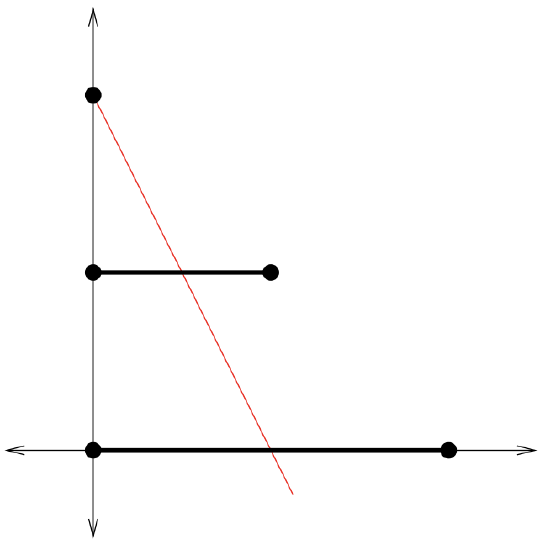
\includegraphics[scale=0.3]{Bisezione.png}
\end{figure}

\vspace{.5cm}

\begin{defn}[Geometria Astratta]
    Una geometria astratta è definita da una coppia di insiemi $(S,L):$ $$\begin{cases}
        S:=\{ Punti \} \\
        L:=\{ Rette \}
    \end{cases} \text{ con } L \subseteq \mathscr{P}(S)/ \{ \emptyset \}$$
Tali che:
\begin{enumerate}
    \item $\exists$ retta per ogni coppia di punti: $\forall A,B \in S \mid A \neq B \quad \exists l \in L\mid A,B \in l$
    \item $\exists$ due punti distinti appartenenti a una retta per ogni retta: $l \in L \Rightarrow \exists A,B \in l|A \neq B$
\end{enumerate}
\end{defn}


\begin{example*}
    Le più semplici geometrie astratte possibili sono dunque $(\emptyset , \emptyset), (\{ a \}, \emptyset)$ e una coppia di punti $( \{ a,b  \} , \{ \{ a,b \} \} )$.
\end{example*}

\begin{defn}[Rette parallele] In geometria astratta
   $l_1,l_2\in L$ allora $l_1//l_2$ se $l_1\cap l_2=\emptyset$ oppure $l_1=l_2$
\end{defn}

\begin{defn}[Geometria Neutra]
 se rispetta solo i primi 4 postulati di Euclide.
 \\
 In absolute geometry, it is also provable that two lines perpendicular to the same line cannot intersect (which makes the two lines parallel by definition of parallel lines) $\implies\exists$ rette parallele
\end{defn}

\begin{defn}[Geometria di Incidenza]
    
Data una Geometria Astratta $(S,L)$ questa è di incidenza se
\begin{enumerate}
    \item Per ogni coppia di punti passa sempre una e una sola retta: $\forall A,B\in S \quad \exists ! l \in L\mid A,B \in l$
    \item Esistono 3 punti per i quali non passa una retta (ovvero non allineati): $\exists A,B,C \in S\mid  \not \exists l \in L \mid A,B,C \in l$
\end{enumerate}
In una geometria di incidenza due rette sono o parallele hanno un punto di incidenza.
\end{defn}


\begin{example*}
    La più semplice geometria di incidenza è formata da tre punti A,B,C e dalle loro coppie come rette. (Nell'immagine i punti sono il rosso, il verde e il blu, le rette sono le loro combinazioni giallo, azzurro e lilla. Posso considerare il nero come l'insieme vuoto e il bianco come l'insieme che contiene sia rosso, sia verde sia blu).
\end{example*}


\begin{figure} [H]
    \centering
    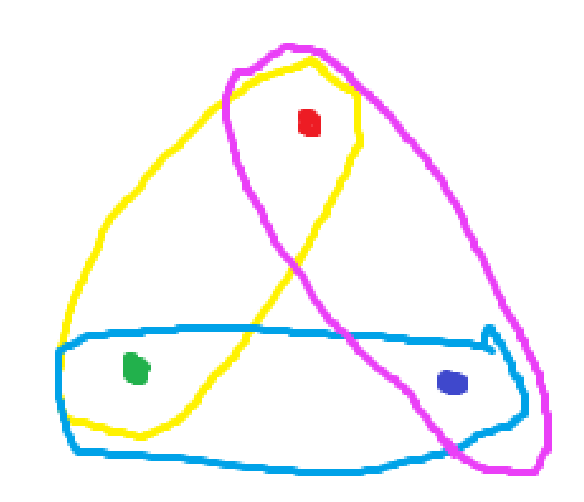
\includegraphics[scale=0.25]{Screenshot 2024-09-18 153852.png}
\end{figure}


\begin{example*}[Piano di Fano]
    Un esempio di geometria di incidenza è il piano di Fano, formato da sette punti e altrettante rette:

\begin{figure}[H]
    \centering
    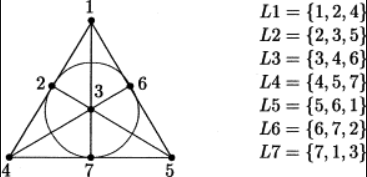
\includegraphics[scale=0.7]{Fano5.png}
\end{figure}

Osservo che ogni coppia di rette possiede uno e un solo punto di incidenza.
\end{example*}

\begin{example*}[Piano di Poincarè - geometria iperbolica] Abbiamo
\begin{align*}
    S&\coloneqq \{ (x,y) \in \re^2|y>0 \} \\
    L&\coloneqq \{ l_a, l_{c,r} \} \quad \text{con} \quad 
    \begin{array}{l}
        l_a:\{ (a,y), y>0 \}   \\
           l_{c,r}=\{ (x,y) \in \re^2| (x-c)^2+y^2=r^2 \land y>0 \}
    \end{array}
\end{align*}
    Dati due punti $A=(x_1,y_1),B=(x_2,y_2)$ $$x_1=x_2 \implies \exists ! l_a=l_{x_1}\mid A,B \in l_a$$ Inoltre se ci passasse una circonferenza questa dovrebbe avere centro su $ \frac{y_1+y_2}{2}>0$ che è assurdo. Se invece $$x_1 \neq x_2 \implies\not \exists a\mid A,B \in l_a$$ invece preso il sistema
$\begin{cases}
(x_1-c)^2+y_1^2=r^2 \\
(x_2-c)^c+y_2^2=r^2 \\
\end{cases}$
ricavo $(x_1+x_2-2c)(x_1-x_2)=(y_1+y_2)(y_1-y_2)$, da questo ricavo c e poi r tornando ad una delle due equazioni precedenti.
\end{example*}

\begin{example*}[Sfera di Riemann - non di incidenza]
    $\begin{cases}
        S=\{x^2+y^2+z^2=1\}\\
        L=\{\text{cerchi di raggio massimo}\}
    \end{cases}$ non è di incidenza perché ad esempio per due poli opposti passano infinite rette
\end{example*}

\begin{defn}[Funzione distanza su $S$]
 $d:S\times S \rightarrow \re$ tale che:
\begin{enumerate}
    \item $d(x,y)\ge 0$
    \item $d(x,y)=0 \iff x=y$
    \item $d(x,y)=d(y,x)$
\end{enumerate}
\end{defn}

\begin{defn}[Sistema di coordinate per una retta] Dati $(S,L)$ e $d$ (funzione distanza assegnata), $$f: l_{\in L} \rightarrow \re$$ è un sistema di coordinate per $l$ se:
\begin{enumerate}
    \item $f$ è biunivoca 
    \item  $\forall P,Q \in l,d(P,Q)=\abs{f(P)-f(Q)}$
\end{enumerate}
ovvero è restrizione sulla retta di $d$ a meno di traslazioni 
\end{defn}

\begin{thm}
    Se $d$ è una metrica per la geometria di incidenza $(S,L)$ tale che:

1) $f:l \rightarrow \re$ suriettiva

2) $\forall P,Q \in l, d(P,Q)=|f(P)-f(Q)|$ 

allora $f$ è sistema di coordinate per $l$
\end{thm} 

\begin{defn}[Geometria Metrica]
    Una geometria metrica è costituita da una terna $(S,L,d)$ dove $(S,L)$ è una geometria di incidenza e $d$ è una funzione distanza per la quale si possa definire un sistema di coordinate $\forall l \in L$

\end{defn}

\begin{rem*}[disuguaglianza triangolare]
    Per il momento la distanza è definita solo internamente alle rette, ignoro dunque la disuguaglianza triangolare
\end{rem*}


\begin{example*}[In geometria euclidea]
    Ad esempio in geometria euclidea ho che le rette verticali hanno come distanza interna 
    $$d(P,Q)= |y_P-y_Q|, f(P)=y_P$$ 
    le rette non verticali $l_{m,q}$ hanno distanza $$d(P,Q)= \sqrt{(1+m^2)(x_P-x_Q)^2}, f(P)=\sqrt{1+m^2} x_P$$
\end{example*}

\begin{example*}[Sul piano di Poincarè]
Sul Piano di Poincarè, dati $P=(x_1,y_1),Q=(x_2,y_2)$ prendo $$d_H(P,Q)\coloneqq\begin{cases}
    \abs{\log{\frac{y_2}{y_1}}} & \text{se }x_1=x_2\\
    \abs{\log{\frac{\frac{x_1-c+r}{y_1}}{\frac{x_2-c+r}{y_2}}}} & \text{altrimenti }
\end{cases}$$

,osservo infatti che $\forall x, x-c+r>0$ poichè $x=c-r \Rightarrow y=0$ che è assurdo.
Pongo ora f(x,y)=t, ricavo $e^t=\frac{x-c+r}{y}$ o $e^{-t}=\frac{y}{x-c+r}=\frac{y}{x-c+r}\frac{x-c-r}{x-c-r}=\frac{y(x-c-r)}{(x-c)^2-r^2}=\frac{y(x-c-r)}{-y^2}=-\frac{x-c-r}{y}. e^t+e^{-t}=\frac{x-c+r}{y}-\frac{x-c-r}{y}=\frac{2r}{y} \Rightarrow cosh(t)=\frac{r}{y}\Rightarrow y=r*sech(t). e^t-e^{-t}=\frac{2(x-c)}{y} \Rightarrow \frac{e^t-e^{-t}}{e^t+e^{-t}}=tanh(t)=\frac{x-c}{r}\Rightarrow x=r*tanh(t)+c$. f è biunivoca tra $l_{c,r} ed \re \Rightarrow d(P,Q)=0 \iff P=Q$
\end{example*}

\begin{rem*}
    Posso avere una geometria di incidenza associata ad una metrica senza sistema di coordinate, ad esempio prendere un sistema di punti e rette euclideo e porre una funzione distanza che opera come l'euclidea su valori minori di 1 e trasforma in 1 ogni distanza maggiore.
\end{rem*}

\begin{proof}
$f(P)=f(Q)\Rightarrow d(P,Q)=0 \Rightarrow P=Q$. Quindi oltre che suriettiva è biunivoca $f$ suriettiva $\Rightarrow \exists ! P_0 \in l |f(P_0)=0$. $d(P,P_0)=|f(P)-f(P_0)|=|f(P)|$ posso associare biunivocamente alla retta un sistema di coordinate, di cui $P_0$ è lo 0
\end{proof}

\begin{example*}[Metrica in cui non vale la disuguaglianza triangolare] Una metrica per il piano euclideo che calcola le distanze in maniera euclidea sulle rette di tipo $l_{m,q}$ e il triplo dell'euclidea sulle rette di tipo $l_a$.

\begin{figure}[H]
    \centering
    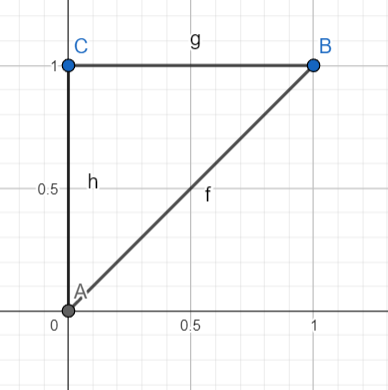
\includegraphics[scale=0.4]{NonEuclidea.png}
\end{figure}

Adottando questa metrica nell'immagine il segmento verticale $AC$ risulta lungo 3, mentre $AB$ risulta $\sqrt{2}$ e $BC$ 1. In questo modo non rispetto la disuguaglianza triangolare
\end{example*}

\begin{thm}   Sia $f$ un sistema di coordinate per una retta $l$ in una geometria metrica. $\forall a \in \re, \epsilon = \pm 1$: $$h(P)\coloneqq f_{a,\epsilon }(P)= \epsilon *(f(P)-a)$$ è un sistema di coordinate per $l$ valido per la stessa metrica $d$ (\hl{infatti $h$ è trasformazione isometrica in quanto ho solo traslato in $a$ e al più invertito il verso})   \end{thm} 

\begin{proof}  $h(P)=t, \exists ! P \in l |f(P) = \frac{t}{\epsilon} +a \Rightarrow$ h è suriettiva. Inoltre prendendo $d(P,Q)=|h(P)-h(Q)|=|\epsilon (f(P)-f(Q))|=|f(P)-f(Q)|\Rightarrow d(P,Q)=0 \iff P=Q$     \end{proof}

\begin{prop}
    Data una retta $l$ e due suoi punti $A,B$ in una geometria metrica, esiste un sistema di riferimento g in cui vale $g(A)=0,g(B)>0$.
\end{prop}
\begin{proof}
    prendendo un sistema arbitrario $f$, creando $h(P)=f(P)-f(A)$ e poi moltiplicando eventualmente per -1.
\end{proof}

\begin{defn}[Punto compreso]
    Data una geometria metrica dico che $B$ è compreso tra $A$ e $C$ se valgono entrambi:
\begin{enumerate}
    \item $\exists l \in L \mid A,B,C \in l (A,B,C)$
    \item $d(A,C)=d(A,B)+d(B,C)$
\end{enumerate}

\end{defn} 

\begin{rem*}[Indipendenza dei due requisiti]
    In metrica $d_1$ (metrica del taxista/taxicab/Manhattan distance, $d(A,B)=\sum_{i=1}^n\abs{A_i-B_i}$ con $A_i$ le componenti cartesiane del punto $A$) ad esempio i punti $A,B,C$ dell'immagine rispettano il secondo requisito ma non il primo.
\end{rem*}

\begin{defn}[Segmento compreso]
    $\overline{AB}\coloneqq\{\text{punti compresi tra $A$ e $B$}\}$
\end{defn}

\begin{gen}[Notazione]
    $A-B-C$ se $B$ sta tra $A$ e $C$
\end{gen}

\begin{thm}   $A-B-C \Rightarrow C-B-A$.   \end{thm} 

\begin{proof}   L'appartenere alla stessa retta è relazione di equivalenza. Cambiando verso di percorrenza della retta la simmetria dell'operatore distanza verifica la proposizione.   \end{proof} 



\begin{thm}  Sia data una geometria metrica e $f,g$ due sistemi di coordinate per la retta $l$. Allora $$ \exists a \in \re\mid\forall P \in l\quad g(P)= \epsilon (f(P)-a)$$    \end{thm} 

\begin{proof}  $\exists ! P_0 \in l|g(P_0)=0,f(P_0)=a. d(P,P_0)=|g(P)-g(P_0)|=|g(P_0)|, d(P,P_0)=|f(P)-f(P_0)|=|f(P)-a|\Rightarrow |g(P)|=|f(P)-a|\Rightarrow g(P)= \epsilon *(f(P)-a)$. Suppongo ora esistano due punti $P_1,P_2 \in l/ \{ P_0 \} | g(P_1)=f(P_1)-a,g(P_2)=-f(P_2)+a \Rightarrow d(P_1,P_2-)=|g(P_1)-g(P_2)|=|f(P_1)+f(P_2)-2a|=|f(P_1)-f(P_2)|\Rightarrow f(P_2)=a,f(P_1)=0\lor f(P_2)=0, f(P_1)=a \Rightarrow \exists P| f(P)=f(P_0)$, assurdo per iniettività delle funzioni    \end{proof} 



\begin{thm}   Data una retta $l$ in una geometria metrica ed $f$ un sistema di coordinate con $f(A)=x,f(B)=y,f(C)=z$: $$A-B-C \iff x<y<z\lor z>y>x$$   \end{thm} 

$d(A,B)=|f(A)-f(B)|=|x-y|, d(A,C)=|f(A)-f(C)|=|x-z|, d(B,C)=|f(B)-f(C)|=|y-z| \Rightarrow |x-z|=|x-y|+|y-z|$ poichè sono allineati (vale proprietà triangolare sull'allineamento)

Ho 6 possibili allineamenti, mostro che di questi reggono logicamente solo i casi in cui ho x-y-z.

Data (S,L,d) geometria metrica e dati tre punti A,B,C appartenenti ad una retta l, solo uno dei tre può essere compreso tra gli altri due. Infatti $\forall A,B| A \neq B \exists C | A-B-C \land \exists D |A-D-B$ poichè assumendo f(A)=x,f(B)=y, $x<\frac{x+y}{2}<y<y+1$ e per suriettività di f esistono C e D tali che $f(C)=y+1,f(D)=\frac{x+y}{2}$

Data f sistema di coordinate per l $A-B-C-D \Rightarrow A-B-C \land B-C-D \land A-B-D \land A-C-D$. Vale per transitività della relazione $<$ sui reali.

Definisco $\overline{AB}=\{ C \in S| C=A \lor C=B \lor A-C-B \}$

Nella geometria di Poincarè un segmento su una retta di tipo $l_{r,c}$ è un arco di circonferenza.

Dato $A \subset S$ un punto B appartenente ad A è detto di passaggio per A se $\exists X,Y \in A|X-B-Y$. Inoltre ho che dato un segmento $\overline{AB}$ A e B sono gli unici due estremi. Lo verifico osservando che per definizione di segmento $z \neq A,B \Rightarrow A-z-B$. Se A è di passaggio per il segmento $\overline{AB}, \exists X,Y \in \overline{AB}|X-A-Y \Rightarrow X-A-Y-B \lor  (X-A-B, \land B=Y) \lor X-A-B-Y$. In tutti e tre i casi osservo come X non sia compreso tra A e B, e non sia uguale nè ad A nè a B, dunque non esiste una simile coppia X,Y.

$\overline{AB} \equiv \overline{CD} \iff d(A,B)=d(C,D)$

Dati A,B, $A \neq B$, $\overrightarrow{AB}=\{ X| X=A \lor A-X-B \lor X=B \lor A-B-X \}$

Ho che $C \in \overrightarrow{AB} \land C \neq A \Rightarrow \overrightarrow{AC}=\overrightarrow{AB}$ (transitività dell'allineamento a destra di un A fissato)

Ho inltre che $C \neq A,B \land C \in \overline{AB} \Rightarrow \overline{AC} \subset \overline{AB}$ per transitività della relazione "stare a sinistra di". 

$\overleftrightarrow{AB}$ è la retta passante per A e B. Poichè data tale retta esiste un sistema di coordinate in cui $f(A)=0 \land f(B)>0\Rightarrow \overrightarrow{AB}=\{ 
x \in \overleftrightarrow{AB} | f(x) \geq 0 \}$.

Sia data la semiretta $\overrightarrow{AB}$ e il segmento $\overline{PQ}, \exists |! C \in \overrightarrow{AB}| \overline{AC} \equiv \overline{PQ}$. Assumendo che P e Q siano distinti (in caso contrario C=A) ho infatti $d(P,Q)=c$, inoltre dato f riferimento per $\overleftrightarrow{AB}, \exists ! C \in AB |f(C)=c$ per biunivocità di f

Ho inoltre che vale $\overline{AB} \equiv \overline{PQ} \land \overline{BC} \equiv \overline{QR} \Rightarrow \overline{AC} \equiv \overline{PR}$

\begin{defn}[Angolo]
    Assumo di avere tre punti A,B,C non allineati (li ho per assioma), definisco $A \hat{B} C=\overrightarrow{BA} \cup \overrightarrow{BC}$
\end{defn}


\begin{thm}  In geometria metrica B è il solo punto estremo di $A \hat{B} C$   \end{thm}

\begin{proof}  $z \neq B$, assumo $z \in \overrightarrow{BA}$ (dimostrazione analoga nel caso $z \in \overrightarrow{BC}$), ho allora $\overrightarrow{BA}=\overrightarrow{Bz} \Rightarrow \exists D \in \overrightarrow{Bz}|B-z-D$ poichè posso trovare un punto D della semiretta su cui f(D)=f(z)+1. Dunque non può esistere un estremo diverso da B. Suppongo ora che B non sia estremo di $A\hat{B}C\Rightarrow \exists X,Y|X-B-Y$ tuttavia osservo che X e Y devono appartenere a semirette distinte (se appartenessero alla stessa e fossero allineati uno dei due verrebbe valutato negativo su f, che è assurdo), ma assumendo che siano su rette distinte, per transitività della relazione di allineamento, ricavo un allineamento tra A,B e C, che è assurdo. dunque B è estremo.    \end{proof} 

\begin{defn}[Triangolo]  $\Delta (A,B,C)= \overline{AB} \cup \overline{BC} \cup \overline{CA}$ è detto triangolo di vertici A,B e C
\end{defn}
\begin{defn}[Insieme convesso] 
$S_1 \subseteq S$ è detto \textbf{convesso} se $P,Q \in S_1 \Rightarrow \overline{PQ} \subseteq S_1$    \end{defn} 

\subsection{ASP e PP}
\begin{axiom}[di Separazione del Piano (ASP)]
    Una geometria metrica $(S,L,d)$ soddisfa l'assioma di separazione del piano se $\forall l \in L \;\exists H_1,H_2 \subset S$, detti semipiani generati da $l$, tali che:
\begin{enumerate}
    \item $S\setminus l=H_1 \cup H_2$
    \item $H_1 \cap H_2= \emptyset$
    \item $H_1,H_2$ convessi
    \item $A \in H_1, B \in H_2 \Rightarrow l \cap \overline{AB} \neq \emptyset$
\end{enumerate}
\end{axiom}

\begin{defn}[Punti dalla stessa parte rispetto una retta]   Due punti/semirette stanno dalla stessa parte rispetto a una retta $l$, in una geometria con ASP, se entrambi appartengono allo stesso semipiano dei due generati da $l$. Tale relazione è di equivalenza.   \end{defn} 

\begin{rem*} dati tre punti $A-B-C$ e una retta $r$ passante per $C$, se i punti non sono allineati su $r$ ho che $A$ e $B$ stanno dalla stessa parte rispetto a $C$.
\end{rem*}
\begin{prop}
   $l  \in L$, se $(H_1,H_2),(H_3,H_4)$ soddisfano entrambe ASP rispetto a $l$, allora le due coppie contengono gli stessi semipiani
\end{prop}


\begin{proof}    $A \in H_1 \Rightarrow A \not \in l \Rightarrow A \in H_3 \lor A \in H_4 \Rightarrow H_1 \subseteq H_3 \lor H_4$ poichè se assumo che abbia punti sia nel primo sia nel secondo il segmento che li congunge interseca l per punto 4 di ASP, ma per il punto 3 ho che $H_1$ è convesso (dunque tutto il segmento gli apparterrebbe) e disgiunto da l. Con lo stesso ragionamento ottengo l'uguaglianza.   \end{proof}

Osservo che per i punti 3 e 4 dell'assioma di separazione del piano $A \in H_1\land B \in H_2 \iff \overline{AB} \cap l \neq \emptyset$

\begin{thm}   Se due rette $l$ ed $l'$ individuano uno stesso semipiano $H_1$ sono la stessa retta   \end{thm} 

\begin{proof}    Per assurdo $l \neq l', l \cap l'$ ha al più un punto. Poichè ogni retta possiede almeno 2 punti $\exists P \in l/l', \exists Q \in l'/l. P=l \cap \overleftrightarrow{PQ}, Q=l' \cap \overleftrightarrow{PQ}.$ Prendo A,B su $\overleftrightarrow{PQ}$ tali che A-P-Q-B. Ne segue che il segmento $\overline{AB}$ interseca l in P, ed l' in Q. Ne segue che A e B stanno da parti opposte sia di l sia di l'. Ne segue che ho un allineamento A-P-Q, con Q appartenente ad l' e sia P sia A dalla stessa parte rispetto ad l'. Se suppongo che A appartenga a $H_1$ (in caso contrario posso ragionare specularmente su B) ne segue che anche P appartiene ad $H_1$, il che è assurdo  \end{proof} 


\begin{rem*}[Geometria senza ASP]
Prendo $(\re^2,L_E)$ una geometria di incidenza euclidea e $\forall l\in L_E\mid l\ne l_0\rightarrow f_l$ sistema di coordinate euclideo, mentre in $l_0$ (retta $x=0$):
$$f_0:l_0\to\re\mid f_0(0,y)\coloneqq
\begin{cases}
    y\quad \text{se }y \not \in \mathbb{Z} \\
    -y\quad \text{se }y\in\mathbb{Z}
\end{cases}\implies d(A,B)\coloneqq\abs{f(A)-f(B)}$$  
    Se prendo il segmento $\overline{(0,1/2)(0,3/2)}$, questo non contiene il punto $(0,1)$ (vedi def. di segmento e punto compreso, evidentemente quella distanza fa casini e per $(0,1)$ non vale $d(A,C)=d(A,B)+d(B,C)$ quindi non è compreso), dunque ha estremi ai due lati della retta ma senza intersecarla, dunque questa geometria con questa metrica non rispetta ASP.
\end{rem*} 

\begin{post}[di Pasch (PP)]\label{axm-pp}
    In una geometria metrica $\forall l \in L,\; \forall \Delta (A,B,C) \quad\exists D \in l \mid A-D-B \Rightarrow l \cap \overline{AC} \neq \emptyset \lor l \cap \overline{BC} \neq \emptyset$
\end{post}

\begin{example*}[Geometria della striscia mancante - no PP]:
\begin{align*}
    S&=\{ (x,y) \in \re^2 \mid x<0 \text{ oppure } x \ge 1 \}\\
    L&=\{ l\cap S \mid l\in L_E,l\cap S\ne\varnothing\}
\end{align*} (L è costituito dalle rette euclidee a cui viene tolta la striscia mancante).  Osservo che posso creare un triangolo euclideo e una retta che attraversa un suo lato normalmente e uno nella striscia mancante, dunque interseca un solo punto del triangolo. La metrica è euclidea ma con i termini a destra della linea mancante shiftati che sostituiscono $x-1$ a $x$ nei conti.   \end{example*} 

\begin{lem*}  Assumo di avere una geometria metrica $(S,L,d)$ con PP. 
$$\begin{cases}
    \text{ $A,B,C$ non sono allineati}\\
    \text{ $A,B,C\notin l$ ognuno}
\end{cases}\implies \text{$l$  non può inters. tutti i lati di $\Delta (A,B,C)$ in un p.to interno}$$
\end{lem*} 

\begin{figure}[H]
    \centering
    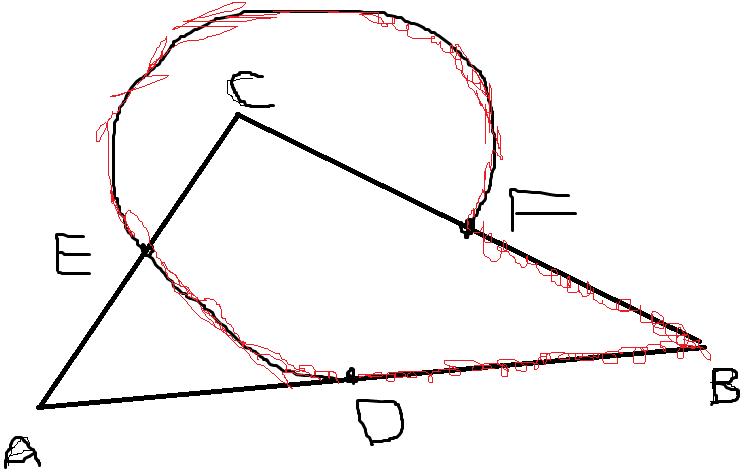
\includegraphics[scale=0.2]{Pasch.png}
\end{figure}

\begin{proof}  .
\begin{itemize}
    \item Assumo $A-D-B,B-F-C,C-E-A$ con $D,E$ ed $F$ appartenenti ad $l$. 
    \item $B,D,F$ non allineati perché non lo sono $A,B,C$. Ho dunque il triangolo $\Delta (B,D,F)$. 
    \item Poichè $l$ passa per $D,E,F$, e vale $D-E-F$ ho che $\overleftrightarrow{AC} \cap \overline{DF}=\{ E \}$. Per postulato \nameref{axm-pp} ho quindi che $$\overleftrightarrow{AC} \cap \overline{BD} \neq \emptyset \lor \overleftrightarrow{AC} \cap \overline{BF} \neq \emptyset$$ 
    
$\overline{BD} \subset \overline{AB} \Rightarrow \overleftrightarrow{AC} \cap \overline{BD} \subset \overleftrightarrow{AC} \cap \overline{AB}=\{ A \}$ ma $A \not \in \overline{BD} \Rightarrow$ L'intersezione è con $\overline{BF}$, ma vale un ragionamento simmetrico con C al posto di A, ho dunque una violazione di Pasch, che è assurdo. \lightning
\end{itemize}    \end{proof} 

\begin{myboxed}
\begin{thm}  $ASP \iff PP$    \end{thm} 
\end{myboxed}

\begin{proof} Doppia implicazione:
\begin{itemize}
    \item[$\implies)$] Prendo  $l|l \cap \overline{AB} =B$. \noun{wlog} assumo inoltre $l \cap \overline{AC} = \emptyset \Rightarrow$ e abbiamo
    $$\begin{cases}
        \text{A e C sono dalla stessa parte di l}\\
        \text{A e B stanno da parti opposte}
    \end{cases}\implies\text{C e B stanno da parti opposte}\overset{\text{ASP}}{\implies} l \cap \overline{BC} \neq \emptyset$$

\begin{figure}[H]
    \centering
    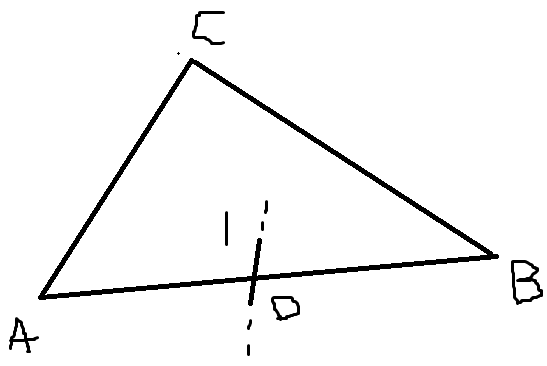
\includegraphics[scale=0.25]{ASPePP.png}
\end{figure}
    \item[$\impliedby)$]
    \begin{itemize}
        \item Data $l \in L, P \not \in l$ definisco $$\begin{array}{l}
         H_1:=\{ Q \in S\mid Q=P \lor \overline{PQ} \cap l = \emptyset \}   \\
         H_2:=\{ Q \in S\mid Q \not \in l \land \overline{PQ} \cap l \neq \emptyset \}
    \end{array}$$ Chiaramente questi due insiemi sono disgiunti (Le caratterizzazioni dei loro punti sono mutuamente esclusive) e la loro unione (per terzo escluso) da S/l. 
    \item Assumo di avere tre punti P,R ed S allineati, di cui $$R,S \in H_1\Rightarrow P=R \lor S=P \lor [R-S-P] \lor [R-P-S] \lor [P-R-S]$$ Osservo ora che $$R-P-S \Rightarrow \overline{RS}=\overline{RP} \cup \overline{PS} \Rightarrow \overline{RS} \subseteq H_1$$ per ipotesi su P. Se P=R o P=S vale lo stesso discorso senza l'unione. Invece $P-R-S \Rightarrow \overline{RS} \subset \overline{PS}$ e vale lo stesso se P-S-R, quindi \textbf{ho che $H_1$ è convesso}. 
    \item Assumo di avere due punti allineati R,S, appartenenti ad $H_2$, con allineamento P-R-S. Osservo che per ipotesi i segmenti $\overline{PR}, \overline{PS}$ intersecano $l$ in un punto. La retta $\overleftrightarrow{PS}$ interseca $l$ in un solo punto, essendo una geometria metrica (quindi d'incidenza), e tale punto deve essere comune a $\overline{PS}$ e $\overline{PR}$, dunque ho che $\overline{RS} \cap l = \emptyset$. Assumo di avere due punti R ed S  non allineati con P appartenenti ad $H_2$, ho che l interseca per ipotesi $\overline{PR},\overline{PS}$, per lemma precedente, se vale PP, l interseca solamente due lati di $\Delta (P,R,S)$ quindi $l \cap \overline{RS} = \emptyset$ quindi \textbf{anche $H_2$ è convesso}. 
    \item Assumo di avere due punti R,S allineati a P tali che $R \in H_1, S \in H_2, R-P-S \lor P-R-S$, osservo che la retta a cui questi punti appartengono interseca una sola volta l, ed in entrambi i casi l'intersezione deve appartenere a $\overline{PS}$. Nel primo caso questo implica automaticamente che l'intersezione appartenga anche ad $\overline{RS}$, mentre nel secondo caso lo implica perchè, se assumessi il contrario, avrei che l'intersezione appartiene a $\overline{PR}$, che è assurdo per definizione di $H_1$. Osservo ora che, dati $R \in H_1, S \in H_2$ non allineati ho che il triangolo $\Delta (P,R,S)$ interseca l nel lato $\overline{PS}$ e non lo interseca nel lato $\overline{PR}$ per ipotesi, inoltre per PP deve intersecare due lati su tre, dunque $l \cap \overline{RS} \neq \emptyset$. Ho quindi che $H_1,H_2$ rispettano tutti i requisiti di ASP. 
    \end{itemize}
    \end{itemize}
\end{proof}



\begin{rem*}[Insiemi convessi con ASP]
    Dato ASP e un insieme convesso $C$ e una retta $l\mid C \cap l = \emptyset$ ho che tutti i punti di $C$ si trovano dalla stessa parte di $l$ (altrimenti dati due punti sui lati opposti il loro segmento dovrebbe intersecare l per ASP).
\end{rem*} 

\begin{prop}    Sia $P \in int(A \hat{B} C)$, la semiretta $\overrightarrow{BP}$ interseca $\overline{AC}$ in uno e un solo punto.  \end{prop} 

\begin{proof}   Essendo geometria metrica $\exists E\mid E-B-C,$ osservo che P e C sono dalla stessa parte rispetto ad $\overleftrightarrow{AB}$ poichè P è interno all'angolo, E e C sono invece da parti opposte, dunque anche E e P, ne segue che $\overrightarrow{BP} \cap \overline{AE}= \emptyset$. Prendo ora $Q|Q-B-P$ ed osservo che A e P si trovano dalla stessa parte rispetto a $\overleftrightarrow{BC}\Rightarrow \overrightarrow{EA} \cap \overrightarrow{BQ} = \emptyset$. Prendo ora $\Delta (E,A,C)$ e $\overleftrightarrow{QP}$ e osservo che quest'ultima è composta da $\overrightarrow{BQ}$ e $\overrightarrow{BP}$, per dimostrazione precedente queste due semirette sono disgiunte da $\overline{EA}$ e, poichè la retta interseca $\overline{EC}$ in B, per PP esiste uno e un solo punto in $\overline{AC}$ che interseca $\overleftrightarrow{BP}$.   \end{proof} 

\begin{figure}[H]
    \centering
    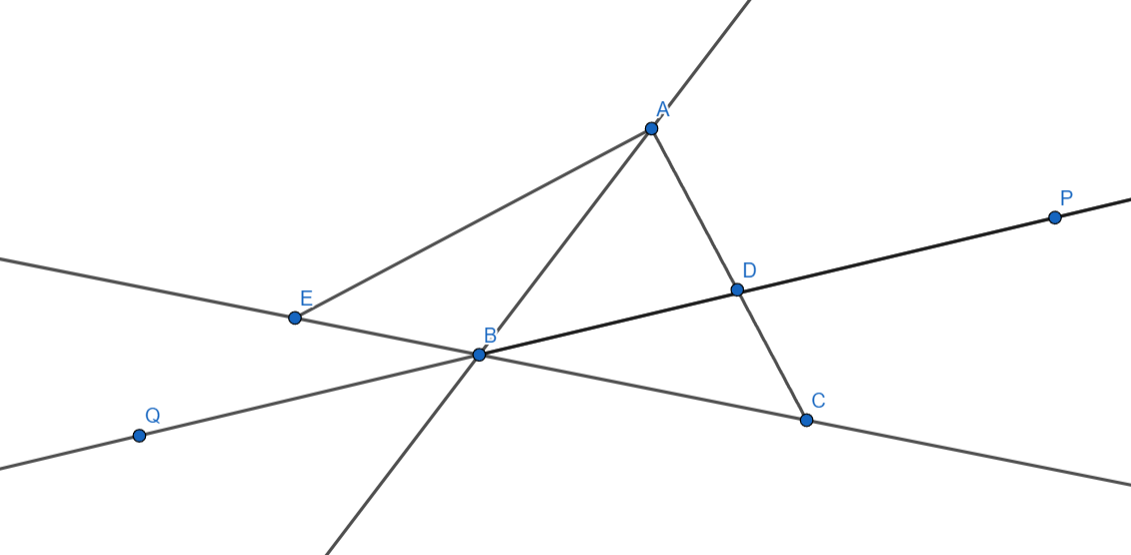
\includegraphics[scale=0.2]{Dimostrazione1.png}
\end{figure}

\begin{defn}[Quadrilatero]  Dati 4 punti $A,B,C,D$ distinti in una geometria di Pasch tali che non costituiscono una terna allineata e $int(\overline{AB})\cap int(\overline{BC}) \cap int(\overline{CD}) \cap int(\overline{DA})= \emptyset \Rightarrow \overline{AB} \cup \overline{BC} \cup \overline{CD} \cup \overline{DA}$ è detto quadrilatero di vertici $A,B,C,D$. \end{defn} 

\begin{defn}[Quadrilatero convesso]  Se ogni lato risulta interamente dalla stessa parte rispetto alla retta su cui giace il lato opposto.     \end{defn} 

\begin{thm}  (Quadrilatero convesso $\iff $ Ogni vertice è interno all'angolo formato dagli altri 3)    \end{thm} $PP \Rightarrow $ 

 In una geometria di Pasch le diagonali di un quadrilatero convesso si intersecano perchè i vertici A e C sono sui lati opposti della retta che contiene B e D e viceversa, quindi $\overline{AC} \cap \overleftrightarrow{BD}= \{ P_1 \} , \overline{BD} \cap \overleftrightarrow{AC}=\{ P_2 \}$ ma $|\overleftrightarrow{AC} \cap \overleftrightarrow{BD}|=1 \Rightarrow P_1=P_2=P$. 
 
 \begin{thm}  Se $ABCD$ è un quadrilatero in una geometria di Pasch e le coppie di lati opposti sono parallele $\implies$ il quadrilatero è convesso    \end{thm} 

 \begin{proof}   $\overline{AB} \cap \overleftrightarrow{CD} = \emptyset $, ragionando specularmente ottengo un semipiano $H_1$ generato da $\overleftrightarrow{CD}$ contenente A ed un semipiano $H_2$ generato da $\overleftrightarrow{AD}$ contenente B. Ne segue che $int(\overline{AB}) \cap \overleftrightarrow{CD} \subset (H_1 \cap H_2) \cap \overleftrightarrow{CD}=\overline{CD}$ per teorema sui semipiani, ma per definizione sui quadrilateri $\overline{AB} \cap \overline{CD}= \emptyset$ quindi il parallelismo implica la convessità.   \end{proof} 

 \begin{lem*}   Data una geometria di Pasch, date una retta $\overleftrightarrow{AB}$ e un segmento $\overline{CD}$ disgiunto da questa, $D \in int(A \hat{B} C) \iff$ A e C stanno da parti opposte rispetto a $\overleftrightarrow{BD}$.   \end{lem*} 

 \begin{proof} Se D è interno all'angolo, per dimostrazioni precedenti so che esiste ed è unico il punto di intersezione tra $\overline{AC}$ e $\overrightarrow{BD}$, dunque ricavo che A e C non possono stare dalla stessa parte, e se assumo che uno dei due sia sulla semiretta contenente sia B sia D nego che D sia interno all'angolo, dunque A e C sono da parti opposte di $\overleftrightarrow{BD}$. Se assumo invece che A e C siano da parti opposte di $\overleftrightarrow{BD}$ ricavo che $\overrightarrow{DA} \cap \overrightarrow{BC} = \emptyset$ per dimostrazione precedente. Prendo ora E tale che E-B-C, ho che si trova dal lato opposto di $\overleftrightarrow{AB}$ rispetto a C, e C si trova dalla stessa parte di D, dunque ho che $\overrightarrow{BE} \cap \overrightarrow{AD} = \emptyset \Rightarrow \overline{AD} \cap \overleftrightarrow{BC}= \emptyset$ mostro così che A e D sono dalla stessa parte rispetto a $\overleftrightarrow{BC}$, posso eseguire un ragionamento analogo per C e D rispetto a $\overleftrightarrow{AB}$ e ricavo che P è interno all'angolo.     \end{proof} 

 \begin{figure}[H]
     \centering
     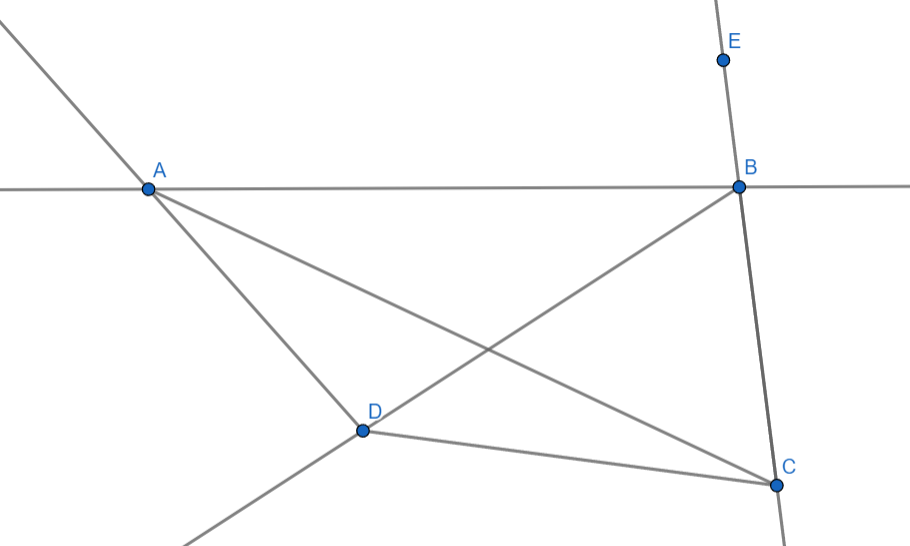
\includegraphics[scale=0.3]{Lemma1.png}
 \end{figure}

 \vspace{.5cm}

\subsection{Geometria angolare}
\begin{defn}[Geometria goniometrica]    Una geometria di Pasch è goniometrica se è definita una \textbf{misura angolare}, ovvero detto $$a=\{\text{tutti gli angoli che si possono costruire}\}$$ allora $\exists m:a\rightarrow (0,r_0)$ tale che:
\begin{enumerate}
    \item $l \in L$ ed un semipiano $H_1$ individuato da $l$, fissati A e B appartenenti ad $l$ e preso $\theta \in (0,r_0), \exists ! \overrightarrow{BH} \in H_1| m(A\hat{B} H)=\theta$
    \item $D \in int(A\hat{B}C) \Rightarrow m(A\hat{B}D)+m(D\hat{B}C)=m(A\hat{B}C)$
\end{enumerate}
\end{defn} 

\begin{rem*}
    Osservo che questa definizione contempla \textbf{solo gli angoli convessi} non contempla né angolo nullo né angolo piatto, essendo l'intervallo $(0,r_0)$ aperto.
\end{rem*}

\begin{defn}[Angolo retto]  Se $m(A\hat{B}C)=\nicefrac{r_0}{2}$  \end{defn} 

\begin{defn}[Angoli adiacenti e opposti]   $A\hat{B}C$ e $C\hat{B}D$ sono adiacenti se $A-B-D$. $A\hat{B}C$ e $A'\hat{B}C'$ sono opposti al vertice se $A-B-A'$ e $C-B-C'$.   \end{defn} 

\begin{thm}  Sia data, in una geometria goniometrica, una retta $\overleftrightarrow{AB}$ e due punti C e D dalla stessa parte rispetto ad essa e tali che $m(A\hat{B}C)<m(A\hat{B}D)\Rightarrow C \in int(A\hat{B}D)$.
    \end{thm} 

    
\begin{proof}   A e C stanno dalla stessa parte rispetto a $\overleftrightarrow{BD}$ poichè se assumo $C \in \overrightarrow{BD}$ ho che i due angoli sono uguali e dunque devono avere la stessa misura, se $A \in \overleftrightarrow{BD}$ non ho C e D dalla stessa parte di $\overleftrightarrow{AB}$ che è assurdo, se invece assumo che A e C siano da parti opposte di $\overleftrightarrow{BD}$ ricavo $m(A\hat{B}D)+m(D \hat{B}C)=m(A\hat{B}C) \Rightarrow m(A\hat{B}D)<m(A\hat{B}C)$ che è assurdo. Ho dunque che A e C stanno dalla stessa parte rispetto a $\overleftrightarrow{BD}$, C e D stanno dalla stessa parte rispetto ad $\overleftrightarrow{AB}$, quindi $C \in A\hat{B}D$.   \end{proof} 

\begin{thm}  $A\hat{B}C$ e $C\hat{B}D$ adiacenti $\Rightarrow m(A\hat{B}C)+m(C\hat{B}D)=r_0$    \end{thm} 

\begin{proof}  Chiamerò le misure degli angoli a e b. 

1)Assumo che $a+b<r_0$, osservo che detto $ H_1$ il semipiano generato da $\overleftrightarrow{AD}$ in cui giace C, vale l'esistenza e unicità di un punto $E\in H_1|m(A\hat{B}E)=a+b\Rightarrow C \in int(A\hat{B}E)$. $m(A\hat{B}C)+m(C\hat{B}E)=a+b \land m(C\hat{B}E)=b \land E \in int(C\hat{B}D) \Rightarrow m(C\hat{B}E)+m(E\hat{B}D)=m(C\hat{B}D) \Rightarrow b+m(E\hat{B}D)=b$ che è assurdo perchè non ho angoli nulli.

2) Assumo invece che $a+b>r_0$, ho comunque che $2*r_0>a+b$ (nessuno dei due termini singoli può essere maggiore di $r_0$) ne segue che $r_0>a+b-r_0. b<r_0 \Rightarrow b-r_0<0 \Rightarrow a+b-r_0<a. \exists F \in int(A\hat{B}C)| m(F\hat{B}C)=r_0-b$. $C \in int(F\hat{B}D)$ poichè F e D sono da parti opposte rispetto a $\overleftrightarrow{BC}$, C e D sono dallo stesso lato rispetto a $\overleftrightarrow{BF}$.$m(F\hat{B}C)+m(C \hat{B}D)=m(F\hat{B}D)=(r_0-b)+b=r_0$ assurdo.
\end{proof} 


\begin{cor}    Gli angoli opposti al vertice hanno la stessa ampiezza. Sono infatti entrambi adiacenti ad uno stesso angolo, dunque la loro somma con quell'angolo deve essere sempre $r_0$, dunque tra loro sono uguali.  \end{cor} 

\begin{thm}   Se in una geometria goniometrica vale $m(A\hat{B}C)+m(C\hat{B}D)=m(A\hat{B}D)$ allora $C \in int(A\hat{B}D)$   \end{thm} 

\begin{proof}  C e D stanno dalla stessa parte di $\overleftrightarrow{AB}$. Suppongo infatti per assurdo che non sia così. Assumo ora che A e D siano dalla stessa parte rispetto a $\overleftrightarrow{BC}$, avrei $\overline{AD} \cap \overleftrightarrow{BC}= \emptyset, \overline{CD} \cap \overleftrightarrow{AB} \neq \emptyset \Rightarrow A \in int(C\hat{B}D) \Rightarrow m(C\hat{B}D)=m(C\hat{B}A)+m(A\hat{B}D)$ ma per ipotesi ho $m(A\hat{B}D)=m(A\hat{B}C)+m(C\hat{B}D)$ ricaverei quindi $m(C\hat{B}A)<0$ che è assurdo. Suppongo invece che A e D stiano da parti opposte rispetto a $\overleftrightarrow{BC}$, allora ho che $\overline{AD} \cap \overleftrightarrow{BC} \neq \emptyset,$ prendo $E \in \overleftrightarrow{AB}|A-B-E.$ E e D sono dalla stessa parte rispetto a $\overleftrightarrow{BC}$, poichè entrambi sono opposti ad A, quindi $\overline{ED} \cap \overleftrightarrow{BC} = \emptyset , \overline{CD} \cap \overrightarrow{BE} \neq \emptyset \Rightarrow E \in int(C \hat{B} D) \Rightarrow m(C\hat{B}E)+m(E\hat{B}D)=m(C\hat{B}D)$ ma $m(A\hat{B}C)+m(C\hat{B}E)=r_0$ poichè A-B-E $\Rightarrow m(C\hat{B}E)=r_0-m(A\hat{B}C)\Rightarrow r_0-m(A\hat{B}C)+m(E\hat{B}D)=m(C\hat{B}D) \Rightarrow m(A\hat{B}C)+m(C\hat{B}D)=m(A\hat{B}D)>r_0$ che è assurdo, ho sbagliato quindi a negare che C e D fossero dalla stessa parte rispetto ad $\overleftrightarrow{AB}$, ne segue per proprietà degli angoli precedentemente dimostrate che $C \in int(A\hat{B}D)$.    \end{proof} 


\begin{defn}[Retta perpendicolare]   Due rette in una geometria goniometrica sono perpendicolari se la loro unione definisce un angolo retto (di ampiezza $r_0/2$).  \end{defn} 

\begin{prop}[Esistenza e unicità retta perp. in geo. goniom.]
    In una \textbf{geometria goniometrica} data una retta $l$, un suo punto B $\exists ! l'\mid B \in l' \land l \perp l'$.  
\end{prop}

\begin{proof}
    In entrambi i semipiani che l genera esiste una semiretta che genera due angoli retti con l, facendo il prolungamento di una di queste genero l'altra per congruenza degli opposti al vertice.
\end{proof}


Data la geometria euclidea e tre punti distinti A,B,C, detti $a= \frac{\overrightarrow{AB}}{|AB|},b=\frac{\overrightarrow{BC}}{|BC|}$ definisco $\theta = \arccos(ab)$. Osservo dunque la funzione $\int_0^1\frac{dt}{\sqrt{1-t^2}}=\pi/2>0$ quindi  $$I(x)=\pi /2 + \int_0^x\frac{1}{\sqrt{1-t^2}}dt$$
è biunivoca da $[-1,1]$ a $[0,\pi]$, definisco la sua inversa come $\cos(x)$. 

\begin{example*}[Angoli in piano di Poincarè]
    In geometria di Poincarè per misurare gli angoli prendo l'angolo tra le rette euclidee tangenti nel punto d'incidenza alle rette di Poincarè.
\end{example*}

\subsection{Congruenza di triangoli - geometria neutra}
\begin{defn}[Congruenza tra triangoli]
    Dati $T_1=\Delta (A,B,C), T_2=\Delta (D,E,F)$ sono congruenti se $\exists f:\{ A,B,C \} \rightarrow \{ D,E,F \}$ tale che:
    \begin{enumerate}
        \item $f$ è biunivoca
        \item )$\overline{f(A)f(B)}\equiv \overline{AB},\; \overline{f(B)f(C)} \equiv \overline{BC},\; \overline{f(C)f(A)}=\overline{CA} \qquad (\equiv$ significa stessa misura)
        \item $m(C\hat{A}B)\equiv m(f(C\hat{A}B))...$
    \end{enumerate}
    ovvero mantiene distanze (isometria) e angoli: roto-traslazione
\end{defn}

\begin{axiom}[Lato-Angolo-Lato (LAL)]\label{axm-lal}
     Due triangoli hanno due lati e l'angolo compreso tra le semirette che questi formano, tra loro congruenti $\implies$ congruenti
\end{axiom} 


\begin{example*}[Controesempio in geometria del taxista]
    Se prendo il piano euclideo con goniometria euclidea e metrica $d_1$ ($d_1=\abs{x_A-x_B}+\abs{y_A-y_B}$) osservo che posso prendere i triangoli $(-1,1)(1,1)(0,0)$ e $(0,2)(0,0)(2,0)$, entrambi hanno due lati lunghi due con in mezzo un angolo retto, ma il primo è equilatero, il secondo ha il terzo lato lungo 4, dunque questa geometria non rispetta \nameref{axm-lal}
\end{example*}

\begin{myboxed}
\begin{rem*}
   Geometria neutra (no quinto postulato) $\implies$ soddisfa LAL. 
\end{rem*}
\end{myboxed}

\begin{myboxed}
\begin{thm}[Pons Asinorum-Ponte dell'asino] \label{thm-pons-ansiorum}Data una geometria neutra gli angoli alla base di un triangolo isoscele sono congruenti.   \end{thm} 
\end{myboxed}

\begin{proof}    Assumo $\overline{AB}=\overline{AC}$, posso definire una\textbf{ funzione che mandi A in sè stesso e inverta B e C}, in questo modo preservo le lunghezze dei due lati congruenti e l'ampiezza dell'angolo in A, dunque per \nameref{axm-lal} gli angoli del primo triangolo sono congruenti a quelli del secondo, quindi i due angoli alla base sono congruenti.  \end{proof} 

\begin{myboxed}
\begin{prop}   $LAL\Rightarrow ALA$ (Angolo-Lato-Angolo)   \end{prop} 
\end{myboxed}

\begin{proof}   .
\begin{itemize}
    \item Assumo di avere due triangoli $\Delta (A,B,C), \Delta (D,E,F)| \overline{AB} \equiv \overline{DE}, \hat{A}=\hat{D}, \hat{B}=\hat{E}$. 
    \item Per assurdo $\overline{AC}\ncong\overline{DF}$, \noun{wlog} $\overline{DF}>\overline{AC} \Rightarrow \exists ! G \in \overline{DF}|\overline{DG} \equiv \overline{AC}$
    \item allora preso $\Delta (D,E,G)$ per LAL è congruente a $\Delta (A,B,C)$, ma essendo G interno a $D\hat{E}F$ ho che $m(D\hat{E}G)<m(D\hat{E}F)=m(A\hat{B}C)$ dunque l'equivalenza tra i due triangoli viene meno, che è assurdo \lightning\end{itemize}  \end{proof} 

\begin{myboxed}
\begin{prop}     $LAL \Rightarrow LLL$ (Lato-Lato-Lato)  \end{prop}
\end{myboxed}

\begin{proof} .
\begin{itemize}
    \item Assumo di avere due triangoli $\Delta (A,B,C), \Delta(D,E,F)$ aventi tutti i lati congruenti 
    \item Prendo la retta $ \overleftrightarrow{AB}$, detto $H_2$ il piano a cui non appartiene $C$ \begin{align*}
        &\exists ! \overrightarrow{AH} \in H_2| B\hat{A}H \equiv E\hat{D}F \\
        &\exists ! C' \in \overrightarrow{AH}| \overline{AC'} \equiv \overline{DF} \quad \text{(l'ho ricostruito specchiato in basso)}
    \end{align*} Per costruzione $\Delta (A,B,C') \equiv \Delta (D,E,F)$ per \nameref{axm-lal}. 
    \item Ne segue che $\Delta (A,B,C)$ e $\Delta (A,B,C')$ hanno i lati congruenti per catena di congruenze (per ipotesi)
    \item Traccio ora il segmento tra C e C' e osservo che i triangoli $\Delta (A,C,C'), \Delta (B,C,C')$ sono isosceli, dunque hanno angoli alla base congruenti per \nameref{thm-pons-ansiorum}. Per somma ho quindi che l'angolo in C e quello in C' sono congruenti, quindi per LAL il triangolo con C e quello con C' sono congruenti, dunque per transitività vale LLL tra $\Delta (A,B,C)$ e $\Delta (D,E,F)$ 
\end{itemize}    \end{proof} 

\begin{myboxed}
\begin{prop}[Esistenza retta perp. in geo. neutra]   In una \textbf{geometria neutra}, data una retta $l$ e un punto $B \not \in l, \exists \;l'|B \in l' \land l' \perp l$.   \end{prop} 
\end{myboxed}

\begin{proof}     Prendo $l=\overleftrightarrow{AC}$ che genera i piani $H_1,H_2.$
$$B \in H_1\implies \begin{cases}
    \exists ! H \in H_2\mid  m(H\hat{A}C)=m(B\hat{A}C)\\
    \exists ! B' \in \overrightarrow{AH}|\overline{AB} \equiv \overline{AB'}
\end{cases}$$ $\{ G\}=\overline{BB'} \cap \overline{AC}.$ Per costruzione ho $\Delta (A,B,G) \equiv \Delta (A,B',G)$ dunque 
$$\text{gli angoli in G sono }\begin{cases}
    \text{congruenti}\\
    \text{adiacenti}
\end{cases}\implies \text{retti}\implies\overleftrightarrow{BB'} \perp \overleftrightarrow{AC}$$ 
\end{proof} 

\begin{figure}[H]
    \centering
    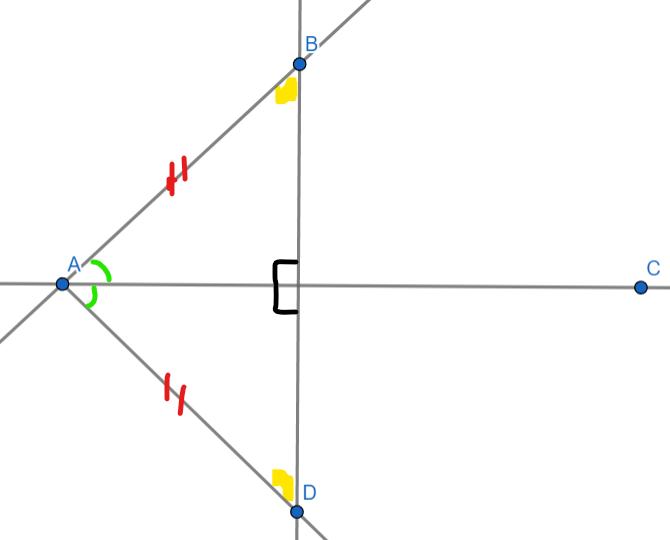
\includegraphics[scale=0.15]{Perp.png}

\end{figure}

\begin{myboxed}
\begin{thm}[dell'angolo esterno]\label{thm-angolo-esterno} In una geometria neutra l'angolo esterno di un triangolo $\Delta (A,B,C)$ è maggiore di ciascuno degli angoli interni non adiacenti.    
\end{thm}
\end{myboxed}

\begin{proof}  .
\begin{itemize}
    \item Prendo $D\mid A-C-D,\quad  \exists ! M \in \overline{BC}|d(B,M)=d(M,C).$ 
    \item Traccio $\overrightarrow{AM}, \quad \exists ! E \in \overrightarrow{AM}| \overline{AM} \equiv \overline{ME}$
    \item $B\hat{M}A \equiv E \hat{M} C$ perché opposti al vertice, dunque per \nameref{axm-lal} $$\Delta (B,M,A) \equiv \Delta (E, M, C) \Rightarrow m(B\hat{C}D)=m(M\hat{C}D)>m(M\hat{C}E)=m(A\hat{B}M)=m(A \hat{B}C)$$
    posso applicare lo stesso ragionamento sull'angolo interno in A, dunque l'angolo esterno in C è maggiore di entrambi.
\end{itemize}    \end{proof} 

\begin{figure}[H]
    \centering
    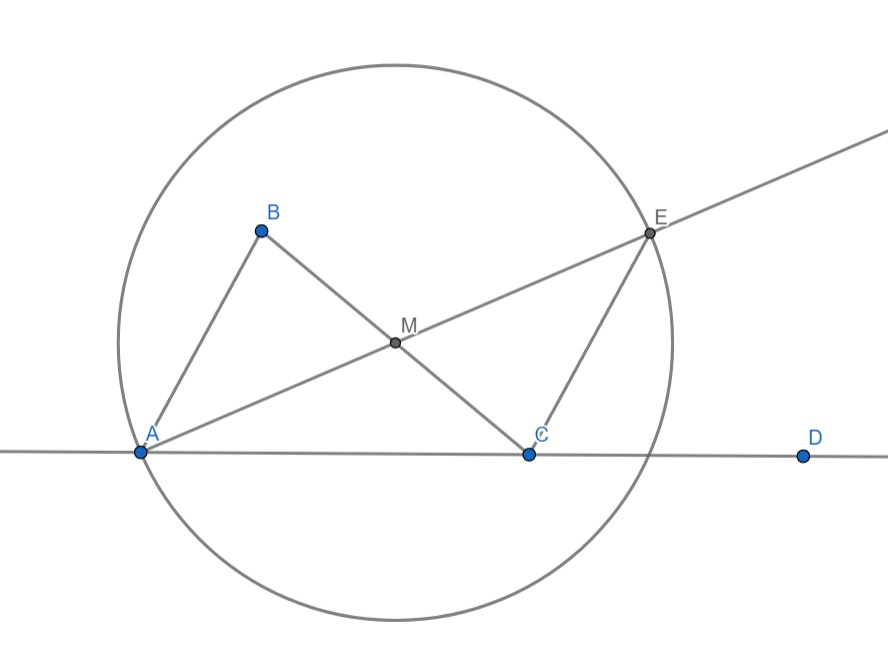
\includegraphics[scale=0.3]{AngoloEsterno.png}
\end{figure}

\begin{myboxed}
\begin{cor}[Unicità della perp. per un punto]  $B \not \in l \Rightarrow \exists !\; l' \mid B \in l' \cap l' \perp l$   
\end{cor} 
\end{myboxed}

\begin{proof}    Suppongo ne esistano due differenti che intersecano l in A ed in C, a quel punto avrei che nel triangolo $\Delta (A,B,C)$ l'angolo esterno in C risulta ampio quanto l'interno in A (poiché sono entrambi $\perp$), contro teo. \nameref{thm-angolo-esterno}\end{proof} 

\begin{example*}[Piano di Moulton-ASP ma non LAL] è un piano euclideo in cui, oltre alle normali rette verticali e alle rette oblique con coefficiente m minore di 0, sono presenti le \textbf{rette di Moulton}, che hanno la forma $y=mx+b$ per $x\leq 0$ e la forma $y= \frac{m}{2}x+b$ per $x>0$, ed hanno $m \geq 0$. Risulta una geometria astratta (esistono 3 punti senza congiungente), di incidenza (Qualunque coppia di punti ha una e una sola coppia di rette che li connetta). Posso anche definire la metrica $$d(P,Q)=\begin{cases}
    d_E(P,Q), P,Q\in L_a^E \cup L_{m,b}^E \lor ((P,Q) \in M_{m,b} \land 0 \leq x_P*x_Q)\\
    d_E(P,B)+d_(B,Q), P,Q \in M_{m,b} \land x_P*x_Q <0
\end{cases}$$
dove B è il punto in cui la retta di Moulton interseca l'asse delle y. Per le rette euclidee si usa un sistema di coordinate f euclideo, per una retta di Moulton si ussa un sistema f in cui il coefficiente m viene  diviso per 2 su $x>0$.\\
Sulle rette euclidee vale ovviamente ASP. Data una retta di Moulton questa definisce $$\begin{cases}
    H_1^+=\{ (x,y)|y>mx+b \} \\
     H_1^-= \{ (x,y)| y<mx+b \}\\
     H_{\frac{1}{2}}^+= \{ (x,y)|y> \frac{m}{2}*x+b \} \\
     H_{\frac{1}{2}}^-= \{ (x,y)| y< \frac{m}{2}*x+b \}
\end{cases}$$ Sulla prima e sulla seconda coppia vale ASP. Definisco $H^+=H_1^+ \cup H_{\frac{1}{2}}^+, H^-=H_1^- \cap H_{\frac{1}{2}}^-$. Posso verificare, usando le rette di Moulton, che rispettano ASP. Per le rette euclidee uso angoli normali, per le rette di moulton se il vertice angolare non è all'intersezione con l'asse delle y ho gli angoli euclidei, in quel caso uso il prolungamento euclideo della retta su $x>0$ come riferimento per definire gli angoli. Osservo ora che posso tracciare due rette euclidee incidenti tra loro e perpendicolari alla stessa retta di Moulton, ne segue che non vale LAL.
\end{example*} 




\begin{myboxed}
\begin{prop}  In una geometria neutra $LAL \Rightarrow AAL$    \end{prop} 
\end{myboxed}

\begin{proof}  .
\begin{itemize}
    \item Assumo di avere $\Delta (A,B,C), \Delta (D,E,F), \hat{C} \equiv \hat{F}, \hat{A} \equiv \hat{D}, \overline{AB} \equiv \overline{DE}$
    \item $$ \overline{AC}<\overline{DF} \Rightarrow \exists G \in \overline{DF}|\overline{DG} \equiv \overline{AC} \Rightarrow \Delta (A,B,C) \equiv  \Delta (D, E, G)$$ per \nameref{axm-lal} $\Rightarrow m(E\hat{G}D)=m(B\hat{C}A)\overset{ip.}{=}m(E\hat{F}G)$ ma così l'angolo esterno in G è congruente all'angolo interno in F rispetto al triangolo $\Delta (E,F,G)$ che è contro teo. \nameref{thm-angolo-esterno}, vale quindi AAL. 
\end{itemize}  \end{proof} 

\begin{prop}
    In una geometria metrica se due lati in un triangolo non sono congruenti non lo sono nemmeno i due angoli opposti e $l_1>l_2 \Rightarrow a_1>a_2$.
\end{prop}
\begin{proof}
 Infatti assumo $\overline{AB} > \overline{AC} \Rightarrow \exists ! D|A-C-D \land \overline{AB} \equiv \overline{AD}. m(A\hat{B}C)<m(A\hat{B}D)=m(A\hat{D}B)<A\hat{C}B$

\begin{figure}[H]
    \centering
    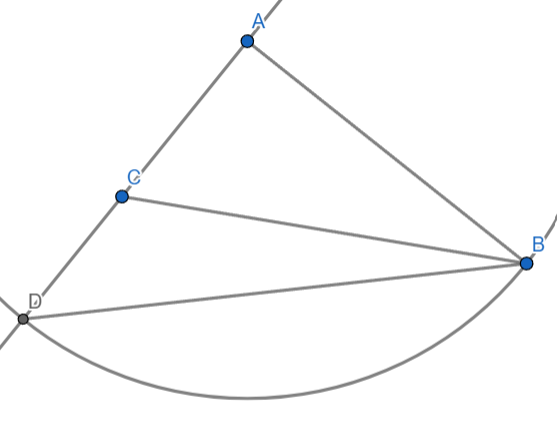
\includegraphics[scale=0.5]{Triangoli1.png}
\end{figure}
\end{proof}

\begin{prop}
    In una geometria neutra vale la disuguaglianza triangolare.
\end{prop}
\begin{proof}
 Infatti dato un triangolo $\Delta (A,B,C), \exists ! D|D-B-C \land \overline{DB} \equiv \overline{AB} \Rightarrow m(A \hat{D} C) =m(D \hat{A}B)<m(D\hat{A}C) \Rightarrow \overline{AC}<\overline{DC} \equiv \overline{BC}+\overline{AB}$ 
\end{proof}

\begin{thm}[della cerniera]
    Dati $\Delta (A,B,C), \Delta (D,E,F)| \overline{AB} \equiv \overline{DE} \land \overline{BC} \equiv \overline{EF} \land \hat{B}>\hat{E} \Rightarrow \overline{AC}> \overline{DF}$
\end{thm}

\begin{proof}   $\exists ! C\hat{B}H \subset C\hat{B}A |m(C \hat{B}H)=m(F\hat{E}D, H \in int(A\hat{B}C) \Rightarrow \overrightarrow{BH} \cap \overline{AC}= \{ K \}), B-H-K \lor H=K \lor B-K-H.$ Prendo $H|\overline{BH} \equiv \overline{AB} \equiv \overline{DE}.$ Prendo $\overrightarrow{BL}$ bisettrice di $A \hat{B} H.$ Questa interseca $\overline{AK}$ in M. Ne segue A-M-K-C e $A \hat{B}M \equiv M \hat{B}H \Rightarrow \Delta (ABM) \equiv \Delta (MBH)$. Osservo ora che per LAL vale anche $\Delta (D,E,F) \equiv \Delta (B,C,H)$, dunque se avessi H=K avrei dimostrato che $\overline{DF} \equiv \overline{HC} <\overline{AC}$. Assumo invece falso A-M-H-C, ricavo $\overline{DF} \equiv \overline{HC} < \overline{HM}+\overline{MC} \equiv \overline{AM}+\overline{MC}=\overline{AC}$ per disuguaglianza triangolare.   \end{proof} 

\begin{figure}[H]
    \centering
    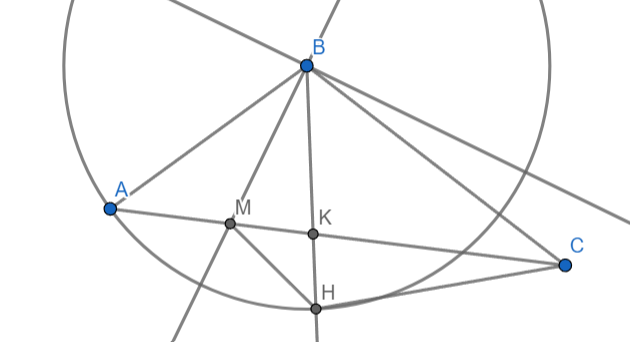
\includegraphics[scale=0.5]{Triangoli2.png}
\end{figure}


Il teorema dell'angolo esterno garantisce di avere sempre solo un angolo retto in geometria neutra, gli altri sono acuti, dunque in geometria  neutra i cateti sono più corti dell'ipotenusa. In geometria neutra se ho due triangoli rettangoli con le ipotenuse ed una coppia di cateti congruenti questi sono congruenti. Infatti dati i triangoli rettangoli $\Delta (A,B,C), \Delta (D,E,F)| \hat{C} \equiv \hat{F}, \overline{AB} \equiv \overline{DE}, \overline{FD} \equiv \overline{AC}$, costruisco $G| E-F-G \land \overline{GF} \equiv \overline{BC}$, per LAL ho così sui cateti e sull'angolo retto go $\Delta (A,B,C) \equiv \Delta (D,F,G) \Rightarrow \Delta (D,E,G)$ è isoscele per equivalenza a catena tra le tre ipotenuse. Ho quindi che gli angoli alla base di $\Delta (D,E,G)$ sono congruenti, quindi lo sono anche $\hat{E}$ e $\hat{B}$, quindi per AAL ho $\Delta (A,B,C) \equiv \Delta (D,F,E)$.

\begin{figure}[H]
    \centering
    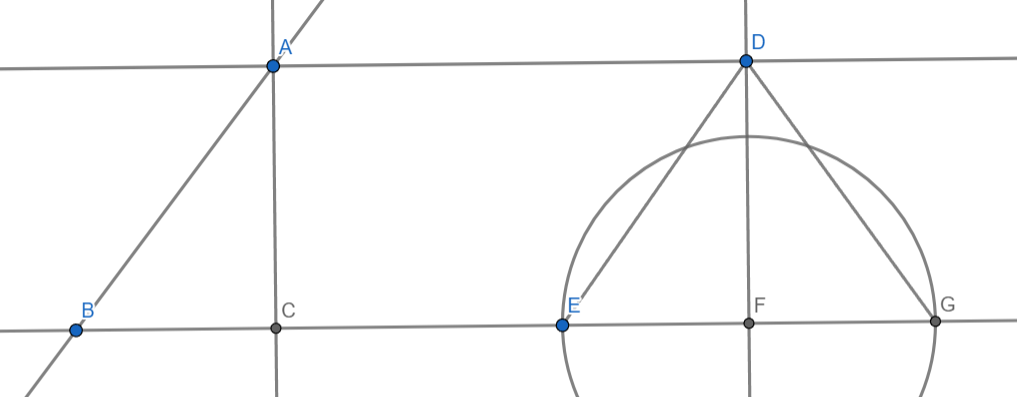
\includegraphics[scale=0.5]{Triangoli3.png}
\end{figure}

\vspace{.5cm}

\begin{myboxed}
\begin{thm}
    In geometria neutra, definite due rette $l_1,l_2$, se esiste una retta $l$ che forma angoli alterni interni congruenti dall'intersezione con queste due ho che $\exists l'| l' \perp l_1 \land l' \perp l_2$.
\end{thm}
\end{myboxed}

\begin{proof}
$m(A \hat{B}E)=m(F \hat{E} B) < \pi /2$. Prendo a questo punto M punto medio di $\overline{BE}$ e P proiezione perpendicolare di M su $\overleftrightarrow{AB}. A-P-B$ altrimenti nel triangolo $\Delta (B,M,P)$ avrei l'angolo acuto esterno $A \hat{B }M<B\hat{P}M$ che è interno e retto. Con lo stesso ragionamento dall'altro lato punto Q|E-Q-F. Per LAA (due angoli retti, due congruenti per ipotesi e ipotenuse uguali per costruzione) ricavo che $ \Delta (P,M,B) \equiv \Delta (E,M,Q)$. Osservo che in $E\hat{M}F$ (dove F può essere un punto arbitrariamente a destra rispetto ad E) esiste ed è unica la semiretta che genera con $\overleftrightarrow{EM}$ un angolo congruente a $P\hat{M}B$, e se tracciassi il prolungamento di $\overline{PM}$ dal lato M questo formerebbe con $\overline{EM}$ un angolo opposto al vertice a $P \hat{M}B$, dunque congruente. Ne segue che il prolungamento di $\overline{PM}$ costituisce quell'unica semiretta. Osservo ora che anche la semiretta $\overline{MQ}$ genera un angolo congruente a $P\hat{M}B$, dunque vale P-M-Q, e la retta $\overleftrightarrow{PQ}$ è ortogonale a $l_1,l_2$.

\begin{figure}[H]
    \centering
    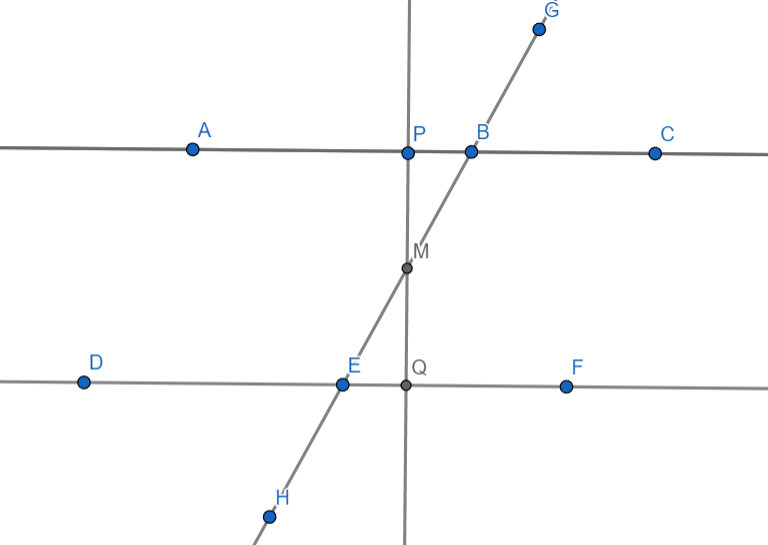
\includegraphics[scale=0.5]{Parallele1.png}
\end{figure}
\end{proof}

\begin{myboxed}
    \begin{cor}[Esistenza parallele]
        geometria neutra $\implies \exists$ retta parallela, data una retta ed un punto esterno ad essa
    \end{cor}
\end{myboxed}
\begin{proof}
    data una retta $r$ ed un punto $P$ esterno ad essa posso \begin{itemize}
        \item tracciare la retta $s$ passante per $P$ e perpendicolare a $r$
        \item tracciare un'altra retta $t$ perpendicolare a $s$ in $P$
    \end{itemize}
    Osservo ora che se $t$ ed $r$ si intersecassero otterrei un triangolo con due angoli interni ed uno esterno retti, violando il teorema \nameref{thm-angolo-esterno} \lightning
\end{proof}

\begin{rem*}[Unicità non garantita]
    Non è però garantita l'unicità della parallela. Infatti se prendo il piano di Poincarè posso vedere che data una retta $l$ ed un punto P ad essa esterno esistono infinite parallele ad $l$ passanti per $P$.
\end{rem*}
\begin{figure}[H]
    \centering
    \includegraphics[scale=0.5]{Poincarè1.png}
\end{figure}

\vspace{.5cm}

\section{Geometrie Euclidee e Non}

\begin{post}[Quinto Postulato di Euclide (QPE)]
    Una geometria goniometrica soddisfa il quinto postulato di Euclide se date tre rette $\overleftrightarrow{BA}, \overleftrightarrow{CD}, \overleftrightarrow{BC}$ con A e D dalla stessa parte rispetto a $\overleftrightarrow{BC}$, $m(A\hat{B}C)+m(B\hat{C}D)<\pi \implies $ $\overleftrightarrow{BA}, \overleftrightarrow{CD}$ si intersecano dalla parte di $\overleftrightarrow{BC}$ dove stanno $A$ e $D$
\end{post}

\begin{rem*}
    Concetto di similitudine e teorema di Pitagora valgono solo se vale il QPE.
\end{rem*}

\begin{post}[Euclideo delle Parallele (PEP)/Playfair Axiom] 
    Una geometria goniometrica soddisfa il postulato euclideo delle parallele se data una retta $l$ e un punto P non appartenente ad essa $\exists ! l' \in L$ passante per $P$ e parallela a $l'$
\end{post} 

\begin{myboxed}
\begin{thm} In geometria neutra (valgono i primi 4 assiomi di Euclide) vale QPE $\iff PEP$ \end{thm} 
\end{myboxed}

\begin{proof}   Abbiamo
\begin{itemize}
    \item[$\implies$] Assumo che sia falso, e di avere due rette l'' ed l' passanti per P e parallele ad l. Traccio una retta r perpendicolare ad l passante per P, assumo che l' ed r siano a loro volta perpendicolari. Poichè le due rette non coincidono, in uno dei due lati rispetto a P una delle rette (assumo l'') genera una semiretta interna all'angolo formato da r ed l'. l ed r formano un angolo retto, l'' ed r un angolo acuto, dunque per QPE l'' ed l si intersecano, che è assurdo.   
    \begin{figure}[H]
    \centering
    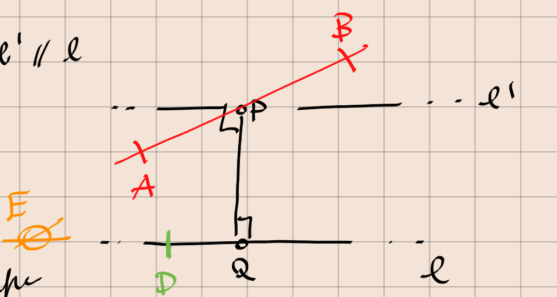
\includegraphics[scale=0.5]{Euclide1.png}
\end{figure}
    \item[$\impliedby$] Suppongo valga PEP di avere 2 rette $\overleftrightarrow{AB}, \overleftrightarrow{CD}, \land m(A \hat{B}C)+m(B\hat{C}D)<\pi $. Costruisco $\overleftrightarrow{BE}, E \in int(D\hat{C}A)|m(C\hat{B}E)=\pi -m(B\hat{C}D) \Rightarrow m(A\hat{B}C)+m(B\hat{C}D)<m(E\hat{B}C)+m(B\hat{C}D)=\pi \Rightarrow \overleftrightarrow{BE}// \overleftrightarrow{CD}$ perchè generano alterni interni congruenti, dunque se si intersecassero violerebbero il teorema dell'angolo esterno. Ne segue per PEP che $\exists P\in \overleftrightarrow{AB} \cap \overleftrightarrow{CD}$, inoltre so che si trova dalla parte di A e D perchè in caso contrario il triangolo formato violerebbe il teorema dell'angolo esterno (angolo in B interno e in C esterno).
\end{itemize}
\end{proof} 

\begin{figure}[H]
    \centering
    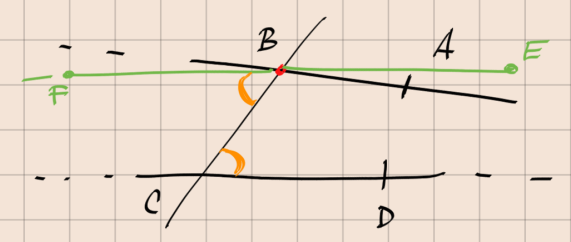
\includegraphics[scale=0.5]{Parallele2.png}
\end{figure}

\textbf{Esempi di geometrie Non-Euclidee:}

\vspace{.5cm}

\textbf{Piano di Poincarè:}

\begin{figure}[H]
    \centering
    \includegraphics[scale=0.25]{Poincarè2.png}
\end{figure}

Osservo che i due angoli evidenziati sono entrambi acuti, stanno su rette di tipo semicerchio rispettivamente di raggio 2 e 3, entrambe centrate in 0, sono dunque parallele.


\textbf{Quadrilateri di Saccheri:}

\begin{figure}[H]
    \centering
    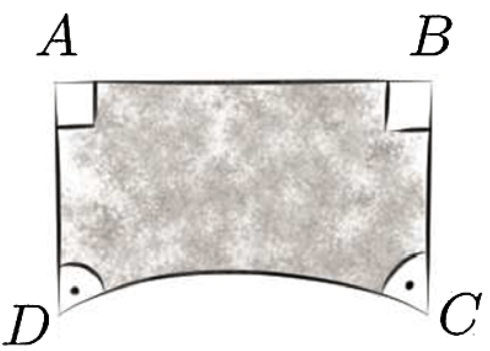
\includegraphics[scale=0.5]{Saccheri1.png}
\end{figure}

Assumo di avere un simile quadrilatero in cui valgono $\overline{AD} \equiv \overline{BC}, \hat{C} \equiv \hat{D}, \hat{A} \equiv \hat{B} = \pi /2$

\begin{myboxed}
\begin{thm}  Dati due quadrilateri di Saccheri ABCD e PQRS con rispettivamente $\overline{AD} \equiv \overline{PS}$ basi euclidee e $\overline{AB} \equiv \overline{PQ}$ i due quadrilateri sono congruenti.    \end{thm} 
\end{myboxed}

\begin{proof}   Osservo subito che per ipotesi ho $\Delta (A,B,D) \equiv \Delta (P,Q,S)$ per LAL. Studio ora $\Delta (B,C,D),\Delta (Q,R,S)$, osservando anzitutto che $\overline{RS} \equiv \overline{QP} \equiv \overline{AD} \equiv \overline{BC}$ per ipotesi. Osservo ora che i due angoli in D ed S sono congruenti poichè complementari agli angoli in D ed S di $\Delta (A,B,D)$ e $\Delta (P,Q,S)$, che sono tra loro congruenti. Osservo infine che $\overline{QS} \equiv \overline{BD}$ per similitudine precedente. Applico dunque LAL e ricavo che questi due triangoli (e dunque i quadrilateri) sono tra loro congruenti.   \end{proof} 

\begin{figure}[H]
    \centering
    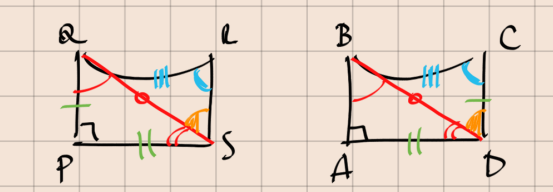
\includegraphics[scale=0.5]{Saccheri2.png}
\end{figure}

\begin{myboxed}
\begin{thm}    Dato un quadrilatero di Saccheri ABCD prendo N ed M punti medi di $\overline{DC},\overline{AB}$.Ho che $\overline{DC} \perp \overline{NM} \perp \overline{AB}$  \end{thm} 
\end{myboxed}

\begin{proof}  .
\begin{itemize}
    \item Traccio $\overline{AN}, \overline{BN}$. Osservo che per \textbf{LAL} ho $\Delta (D,A,N) \equiv \Delta (B,C,N) \Rightarrow \overline{AN} \equiv \overline{BN} \Rightarrow \Delta (A,N,M) \equiv \Delta (B,N,M)$ per \textbf{LLL}. ne segue che i due angoli in M sono congruenti ed adiacenti, dunque sono retti.
    \item So inoltre che $A\hat{N}M \equiv B \hat{N}M, A\hat{N}D \equiv B \hat{N}C \Rightarrow D \hat{N}M \equiv C \hat{N} M$ inoltre sono adiacenti, dunque sono entrambi retti. Ne segue che $\overline{NM}$ è perpendicolare ai due lati.
\end{itemize}   \end{proof} 

\begin{figure}[H]
    \centering
    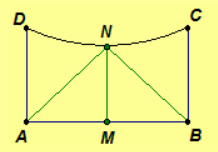
\includegraphics[scale=0.5]{Saccheri.png}
\end{figure}

\hl{Per teorema dell'angolo esterno ricavo quindi che le rette su cui giacciono $\overline{DC}$ e $\overline{AB}$ sono parallele.}

\begin{thm} Dati n punti $P_1...P_n$ in una geometria metrica $d(P_1,P_n) \leq \sum_{i=1}^{n-1} d(P_i,P_{i+1})$     \end{thm} 

\begin{proof}  Vale la disuguaglianza triangolare (caso banale dell'induzione), suppongo valga al passo n, sfrutto la disuguaglianza triangolare per mostrare che vale al caso n+1    \end{proof} 

\begin{thm}  In un quadrilatero di Saccheri $A_1A_2B_2B_1$ di base $\overline{A_1A_2}$ ho che $\overline{B_1B_2} \geq \overline{A_1A_2}$.   \end{thm} 
\begin{proof}
\begin{figure}[H]
    \centering
    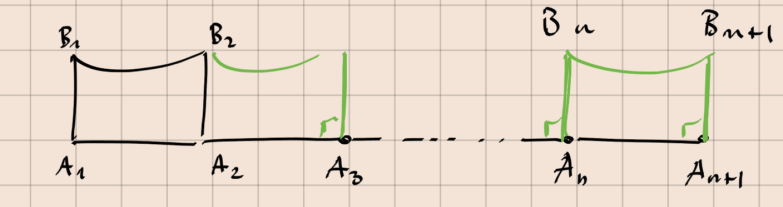
\includegraphics[width=0.3\linewidth]{Saccheri3.png}
\end{figure}
   Traccio una successione di quadrilateri di saccheri tali che   $\overline{B_iA_i}\equiv \overline{A_1B_1}, \overline{A_1A_2} \equiv \overline{A_iA_{i+1}}$. Osservo così che $d(A_1,A_n) \leq d(A_1,B_1)+\sum_{i=1}^{n-1}d(B_i,B_{i+1})+d(B_n,A_n)$ poichè gli $A_i$ sono allineati ho che $d(A_1,A_n)=(n-1)d(A_1,A_2) \leq 2*d(A_1,B_1)+(n-1)d(B_1,B_2) \Rightarrow d(A_1,A_2)-d(B_1,B_2) \leq \frac{2d(A_1,B_1)}{n-1} \forall n \in \mathbf{N} \Rightarrow d(B_1,B_2) \geq d(A_1,A_2)$ 
\end{proof}



Poichè a lato maggiore corrisponde angolo maggiore ho che in una geometria metrica, dato un quadrilatero di Saccheri vale $m(A\hat{B}D) \leq m(B \hat{D}C)$

\begin{myboxed}
\begin{prop} In geometria neutra la somma degli angoli interni di un triangolo è $\le \pi$. \\ \end{prop} 
\end{myboxed}
\begin{figure}[H]
    \centering
    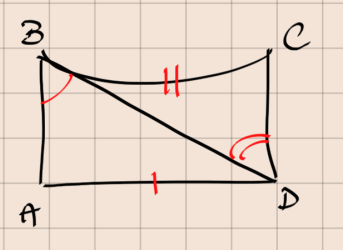
\includegraphics[scale=0.3]{Saccheri4.png}
\end{figure}
\begin{proof}   Dato $\Delta (A,B,D)$ retto in A prendo la verticale passante per D tale che A-D-C e prendo C che le appartiene, tale che $\overline{DC} \equiv \overline{AB}. m(A\hat{D}B)+m(B\hat{D}C)= \pi /2 \Rightarrow m(A \hat{B}D)+m(A \hat{D}B) \leq m(B \hat{D}C)+m(A \hat{D}B)= \pi /2 \Rightarrow$ la somma degli angoli interni di $\Delta (A,B,C)$ non può superare $\pi $. (Con il quinto postulato mostro che è esattamente $\pi $).   \end{proof} 

\begin{figure}[H]
    \centering
    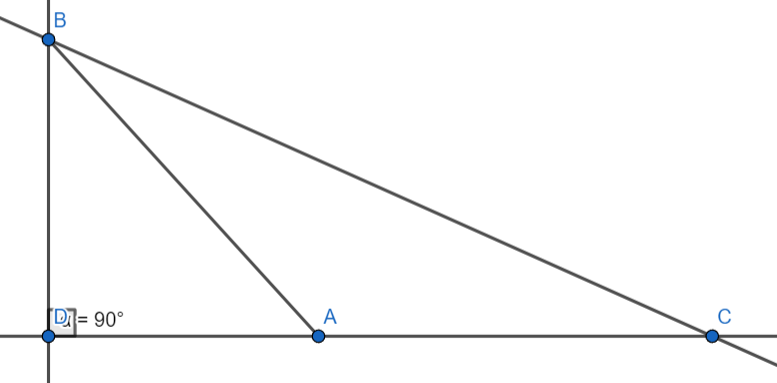
\includegraphics[scale=0.25]{Triangoli4.png}
\end{figure}

Prendo un triangolo $\Delta (A,B,C)| \overline{AC} \geq \overline{AB},\overline{BC}$. traccio la retta passante per B e perpendicolare ad $\overleftrightarrow{AC}$. Osservo che il punto di intersezione D appartiene ad $\overline{AC}$ poichè in caso contrario avrei $\overline{AB}> \overline{AD}, \overline{BC}> \overline{DC} \Rightarrow \overline{AC}= \overline{DC}-\overline{AD} \Rightarrow \overline{AC} < \overline{DC} < \overline{BC}$ che  è assurdo.
Ho dunque A-D-C per costruzione, inoltre $m(A \hat{B}D)+m(B \hat{A}D) \leq \pi /2$ poichè $\Delta (A,B,D)$ è rettangolo in D. Stesso ragionamento per gli angoli in B e C per il triangolo $\Delta (B,C,D)$, ottengo così, sommando gli angoli dei due triangoli, che la loro somma è minore di $\pi$, dunque in geometria metrica la somma degli angoli interni di un triangolo è minore di $\pi$.

\begin{thm}  In geometria euclidea la somma degli angoli interni di un triangolo è esattamente $\pi$.    \end{thm} 

\begin{proof}  $\exists ! l|B \in l \land l//\overleftrightarrow{AC}$. Prendo $D,E \in l|D-B-E. D\hat{B}A \equiv B \hat{A}C, C \hat{B}E \equiv B \hat{C}A$\\
La somma degli angoli interni del triangolo $\Delta (A,B,C)$ è uguale alla somma di tre angoli che dividono un piano, dunque $ \pi$.\end{proof} 



\begin{figure}[H]
    \centering
    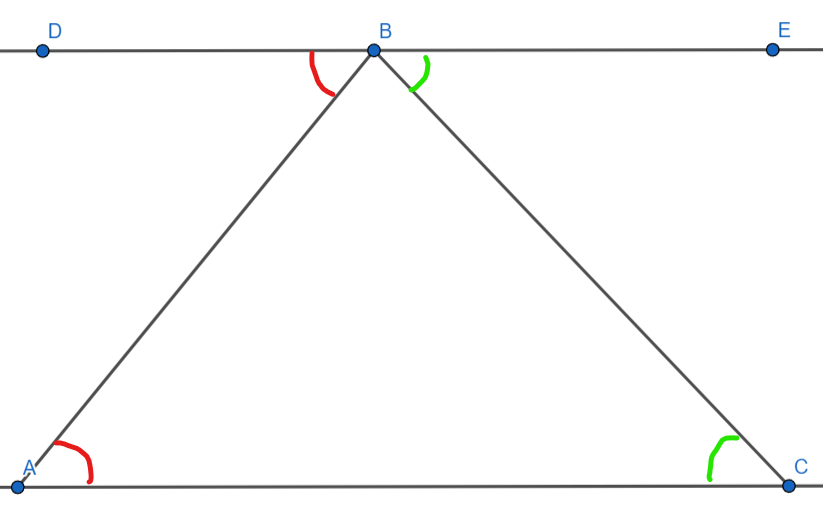
\includegraphics[scale=0.25]{Triangoli5.png}
\end{figure}

In un quadrilatero di Saccheri i due triangoli che lo formano hanno somma degli angoli interni minore di $\pi$.

\begin{myboxed}
\begin{thm}  Data una geometria neutra traccio una retta $l$, definisco un punto $P$ che non le appartenga e traccio l'unica retta passante per $P$ e perpendicolare ad $l$, che interseca in $D$. Prendo dunque un punto $C\mid m(D\hat{P}C) \geq \pi /2$ Ho che $\overrightarrow{PC} \cap l = \emptyset$    
\end{thm} 
\end{myboxed}

\begin{proof}    così non fosse genererei un triangolo con un angolo retto ed uno ottuso, dunque la somma degli angoli interni supererebbe $\pi$, che è assurdo.

Definisco ora $K(P,l):= \{ r \in \re| \exists \overrightarrow{PC} | \overrightarrow{PC} \cap l \neq \emptyset \land m(D \hat{P} C)=r \} , r(P,l)=sup(K(P,l))$. D è la proiezione di P su l, C un punto arbitrario di l. In geometria neutra tale sup esiste sempre perchè K ha come upper bound sempre $\pi /2$, come lower bound 0, e vale l'"assioma" di Dedekind.  \end{proof} 

\begin{thm}   Dati due punti $P,P'$ e due rette $l,l'$ a cui non appartengono, in una stessa geometria neutra, $d(P',l')=d(P,l) \Rightarrow r(P,l)=r(P',l')$    \end{thm} 

\begin{proof}
    Posso osservare che dato un qualunque angolo $a|a \in K(P,l)$, detta D la proiezione di P su l e Q  il punto di intersezione tra la semiretta di angolo a e la retta l, ho che posso prendere un segmento $\overline{D'Q'} \equiv \overline{DQ}$ sulla retta l', applicare LAL (ho un lato congruente per costruzione, uno per ipotesi e l'angolo in mezzo retto per costruzione). Posso eseguire un ragionamento simmetrico e ne segue che $K(P,l)=K(P',l')\Rightarrow r=r'$.
\end{proof}

In un piano di Poincarè prendo $P=(a,b)$, $l$ la verticale passante per l'origine, $a$ positivo. La parallela a $l$ passante per P che generi l'angolo minimo con punti esterni alla semicirconferenza è la verticale passante per $P$ (Qualunque altra retta che provasse a generare un angolo minore dovrebbe essere una semicirconferenza a cui appartengono P e un punto compreso tra la verticale passante per P , la verticale passante per l'origine e che si trovi esternamente alla semicirconferenza centrata nell'origine e di raggio $\overline{OP}$, tale semicirconferenza avrebbe certamente un raggio maggiore di $\overline{OP}$, e poichè P le appartiene dovrebbe avere un centro ad ascissa negativa minore del proprio raggio. Ne segue che, poichè sicuramente esistono punti ad ascissa nulla che distano meno del raggio da questo centro e punti che sicuramente distano di più esiste anche un punto di intersezione). Dal lato interno alla semicirconferenza, invece, la semiretta minore è generata dalla semicirconferenza passante sia per P sia per l'origine, per ragioni geometriche.




\end{document}
